% =============================================================================
%  Adversarial Neural Cryptography — Theoretical Report
%  Complete Report --- Sections 1--12
%
%  Compiler : pdfLaTeX  (TeXstudio default)
%  Class    : article   (switch to IEEEtran for IEEE style if preferred)
% =============================================================================

\documentclass[12pt, a4paper]{article}

% ── Encoding & fonts ──────────────────────────────────────────────────────────
\usepackage[T1]{fontenc}
\usepackage[utf8]{inputenc}
\usepackage{lmodern}               % crisp vector fonts
\usepackage{microtype}             % better justification & hyphenation

% ── Page geometry ─────────────────────────────────────────────────────────────
\usepackage[
  top    = 2.5cm,
  bottom = 2.5cm,
  left   = 3.0cm,
  right  = 2.5cm
]{geometry}

% ── Mathematics ───────────────────────────────────────────────────────────────
\usepackage{amsmath, amssymb, amsthm}
\usepackage{mathtools}             % dcases, prescript, etc.
\usepackage{bm}                    % bold math symbols

% ── Graphics & colour ─────────────────────────────────────────────────────────
\usepackage[dvipsnames, table]{xcolor}
\usepackage{graphicx}
\usepackage{tikz}
\usetikzlibrary{shapes.geometric, arrows.meta, positioning, shadows}

% ── Tables ────────────────────────────────────────────────────────────────────
\usepackage{booktabs}
\usepackage{tabularx}
\usepackage{array}
\usepackage{multirow}

% ── Code listings ─────────────────────────────────────────────────────────────
\usepackage{listings}
\usepackage{lstautogobble}

% ── Section & heading style ───────────────────────────────────────────────────
\usepackage{titlesec}
\usepackage{titletoc}

% ── Header / footer ───────────────────────────────────────────────────────────
\usepackage{fancyhdr}

% ── Hyperlinks & PDF metadata ─────────────────────────────────────────────────
\usepackage[
  colorlinks = true,
  linkcolor  = NavyBlue,
  citecolor  = NavyBlue,
  urlcolor   = NavyBlue,
  pdftitle   = {Adversarial Neural Cryptography — Theoretical Report},
  pdfauthor  = {},
  bookmarks  = true
]{hyperref}

% ── References ────────────────────────────────────────────────────────────────
\usepackage[numbers, sort&compress]{natbib}

% ── Miscellaneous ─────────────────────────────────────────────────────────────
\usepackage{enumitem}
\usepackage{caption}
\usepackage{subcaption}
\usepackage{float}
\usepackage{setspace}
\usepackage{parskip}
\usepackage{tcolorbox}
\tcbuselibrary{skins, breakable, theorems}
\usepackage{mdframed}
\usepackage{soul}                  % \hl{} highlighting
\usepackage{etoolbox}

% =============================================================================
%  COLOUR  DEFINITIONS
% =============================================================================
\definecolor{NavyBlue}   {HTML}{1F4E79}
\definecolor{SteelBlue}  {HTML}{2E75B6}
\definecolor{LightBlue}  {HTML}{D6E4F0}
\definecolor{MidBlue}    {HTML}{BDD7EE}
\definecolor{CodeRed}    {HTML}{C7254E}
\definecolor{CodeBg}     {HTML}{F8F8F8}
\definecolor{DarkGray}   {HTML}{2E2E2E}
\definecolor{LightGray}  {HTML}{F2F2F2}
\definecolor{BorderGray} {HTML}{CCCCCC}
\definecolor{GreenOK}    {HTML}{27AE60}
\definecolor{RedWarn}    {HTML}{E74C3C}

% =============================================================================
%  SECTION  HEADING  STYLES
% =============================================================================
\titleformat{\section}
  {\color{NavyBlue}\normalfont\Large\bfseries}
  {\thesection.}{0.6em}{}
  [\vspace{-4pt}\color{SteelBlue}\rule{\linewidth}{1.2pt}\vspace{2pt}]

\titleformat{\subsection}
  {\color{SteelBlue}\normalfont\large\bfseries}
  {\thesubsection}{0.6em}{}

\titleformat{\subsubsection}
  {\color{DarkGray}\normalfont\normalsize\bfseries\itshape}
  {\thesubsubsection}{0.6em}{}

\titlespacing*{\section}      {0pt}{18pt}{8pt}
\titlespacing*{\subsection}   {0pt}{14pt}{5pt}
\titlespacing*{\subsubsection}{0pt}{10pt}{3pt}

% =============================================================================
%  HEADER / FOOTER
% =============================================================================
\pagestyle{fancy}
\fancyhf{}
\renewcommand{\headrulewidth}{0.5pt}
\renewcommand{\headrule}{\hbox to\headwidth{\color{BorderGray}\leaders\hrule height \headrulewidth\hfill}}
\fancyhead[L]{\small\color{gray}\textit{Adversarial Neural Cryptography — Theoretical Report}}
\fancyhead[R]{\small\color{gray}\thepage}
\fancyfoot[C]{}

% =============================================================================
%  TCOLORBOX  ENVIRONMENTS
% =============================================================================

%% Research question / key insight box
\tcbset{
  researchbox/.style={
    enhanced,
    breakable,
    colback    = LightBlue,
    colframe   = SteelBlue,
    colbacktitle = NavyBlue,
    coltitle   = white,
    fonttitle  = \bfseries\small,
    boxrule    = 0.8pt,
    arc        = 4pt,
    left       = 8pt,
    right      = 8pt,
    top        = 6pt,
    bottom     = 6pt,
    drop shadow,
  }
}

%% Contribution / objective box
\tcbset{
  contribbox/.style={
    enhanced,
    breakable,
    colback    = LightGray,
    colframe   = NavyBlue,
    colbacktitle = NavyBlue,
    coltitle   = white,
    fonttitle  = \bfseries\small,
    boxrule    = 1.2pt,
    leftrule   = 4pt,
    arc        = 2pt,
    left       = 8pt,
    right      = 8pt,
    top        = 5pt,
    bottom     = 5pt,
  }
}

%% Code inline style
\tcbset{
  codebox/.style={
    enhanced,
    colback    = CodeBg,
    colframe   = BorderGray,
    boxrule    = 0.4pt,
    arc        = 2pt,
    left       = 6pt, right = 6pt,
    top = 3pt,  bottom = 3pt,
    fontupper  = \small\ttfamily,
  }
}

% =============================================================================
%  CODE  LISTING  STYLE
% =============================================================================
\lstdefinestyle{python}{
  language         = Python,
  basicstyle       = \ttfamily\small,
  keywordstyle     = \color{NavyBlue}\bfseries,
  stringstyle      = \color{GreenOK},
  commentstyle     = \color{gray}\itshape,
  numberstyle      = \tiny\color{gray},
  numbers          = left,
  stepnumber       = 1,
  numbersep        = 8pt,
  backgroundcolor  = \color{CodeBg},
  showstringspaces = false,
  breaklines       = true,
  frame            = single,
  framerule        = 0.4pt,
  rulecolor        = \color{BorderGray},
  tabsize          = 4,
  captionpos       = b,
  autogobble       = true,
  xleftmargin      = 12pt,
  xrightmargin     = 4pt,
  aboveskip        = 8pt,
  belowskip        = 8pt,
}
\lstset{style=python}

% =============================================================================
%  CUSTOM  COMMANDS
% =============================================================================
\newcommand{\alice}{\textsc{Alice}}
\newcommand{\bob}{\textsc{Bob}}
\newcommand{\eve}{\textsc{Eve}}
\newcommand{\cipher}{\mathcal{C}}
\newcommand{\plain}{\mathcal{P}}
\newcommand{\key}{\mathcal{K}}
\newcommand{\thetaA}{\theta_{\!A}}
\newcommand{\thetaB}{\theta_{\!B}}
\newcommand{\thetaE}{\theta_{\!E}}
\newcommand{\Lbone}{L_{\textsc{B}}}
\newcommand{\Leve}{L_{\textsc{E}}}
\newcommand{\Lab}{L_{\textsc{AB}}}
\newcommand{\code}[1]{\texttt{\color{CodeRed}#1}}
\newcommand{\term}[1]{\textit{#1}}
\newcommand{\N}{N}                 % message/key size

% Shorthand for "bits wrong"
\newcommand{\bw}[1]{#1\,\text{bits wrong}}

% =============================================================================
%  DOCUMENT  METADATA
% =============================================================================
\title{%
  \vspace{-1.5cm}
  {\color{NavyBlue}\rule{\linewidth}{2pt}}\\[6pt]
  {\color{NavyBlue}\LARGE\bfseries
    Learning to Protect Communications\\[4pt]
    with Adversarial Neural Cryptography}\\[6pt]
  {\color{SteelBlue}\large\itshape Theoretical Report}\\[4pt]
  {\color{NavyBlue}\rule{\linewidth}{2pt}}\\[4pt]
  {\normalsize\color{gray}
    Based on Abadi \& Andersen (2016)~\cite{abadi2016learning}\\
    Implementation: \code{main\_enhanced.py} — TensorFlow 2.x $\cdot$ Keras}
}

\author{}   % fill in your name
\date{}

% =============================================================================
\usepackage{tikz}
\usetikzlibrary{calc}
\begin{document}
% =============================================================================

\maketitle
\thispagestyle{fancy}

\vspace{0.3cm}
{\color{BorderGray}\rule{\linewidth}{0.5pt}}
\vspace{-0.2cm}

% Quick-reference info table
\begin{center}
\small
\begin{tabular}{@{} l l @{\hspace{2cm}} l l @{}}
  \textbf{Subject}      & Neural Cryptography &
  \textbf{Framework}    & TensorFlow 2.x \\[2pt]
  \textbf{Reference}    & arXiv:1610.06918    &
  \textbf{Sections}     & 1.\;Abstract \quad 2.\;Introduction \\[2pt]
  \textbf{Keywords}     & \multicolumn{3}{l}{%
    adversarial training · neural encryption · Alice–Bob–Eve ·
    convolutional networks · self-attention}
\end{tabular}
\end{center}

{\color{BorderGray}\rule{\linewidth}{0.5pt}}
\vspace{0.4cm}

% Table of Contents (optional — comment out for submission)
\tableofcontents
\vspace{1cm}

% =============================================================================
\newpage
\section{Abstract}
\label{sec:abstract}
% =============================================================================

\begin{tcolorbox}[
  researchbox,
  title = {\faIcon\ Overview},
  title = {Overview},
]
This report presents a comprehensive theoretical investigation of
\textbf{adversarial neural cryptography} — a paradigm in which neural
networks autonomously learn to encrypt and decrypt communications
\emph{without any prescribed cryptographic algorithm}.
The work is grounded in the landmark study of Abadi and
Andersen~\cite{abadi2016learning} and is accompanied by a full
TensorFlow~2.x implementation in \code{main\_enhanced.py}, which
realises the theoretical system described throughout this report.
\end{tcolorbox}

\vspace{0.4cm}

The system models a three-party communication scenario involving a sender
(\alice{}), a legitimate receiver (\bob{}), and a passive adversary (\eve{}).
\alice{} and \bob{} share a secret key $K \in \{-1,+1\}^{K_{\text{size}}}$
and are jointly optimised — via stochastic gradient descent using the Adam
optimiser~\cite{kingma2014adam} — to minimise \bob{}'s message reconstruction
error while simultaneously maximising \eve{}'s reconstruction error.
\eve{} is trained competitively and independently, receiving a configurable
number of training steps per round to approximate the strongest possible
eavesdropping attack.

The core network architecture — termed \textbf{``mix~\&~transform''} by
Abadi and Andersen — consists of a fully-connected (FC) layer that blends
the plaintext and key representations, followed by four one-dimensional
convolutional layers, all with stride=1 and SAME padding, and sigmoid/tanh
activations. This design allows the network to learn locality and bit-mixing
as \emph{emergent properties}, rather than encoding them by construction.
All three agents share this architecture; \eve{} is structurally
disadvantaged by receiving only the ciphertext as input, with no access
to the shared key.

The loss functions are carefully designed around an important insight: the
target for \eve{} is \emph{indistinguishability from a random guess}, not
maximum error. For $\N$-bit messages, random guessing yields $\N/2$ bits
wrong on average. The quadratic adversarial penalty:
%
\begin{equation}
  \mathcal{L}_{\text{adv}}
  \;=\;
  \frac{\bigl(\tfrac{N}{2} - \|\mathbf{p} - \hat{\mathbf{p}}_E\|_1\bigr)^2}
       {\bigl(\tfrac{N}{2}\bigr)^2}
  \label{eq:adv_loss_abstract}
\end{equation}
%
encodes this goal smoothly, placing strong gradient pressure on \alice{}
and \bob{} when \eve{} is close to the random-guessing threshold.

The implementation, \code{main\_enhanced.py}, is built on
TensorFlow~2.x using Keras model subclassing and eager execution with
\code{@tf.function} compilation. It supports model checkpointing and
reloading, post-training \eve{} robustness evaluation via multiple
reset-and-retrain cycles, real ASCII text encryption
via block-based chunking, a configurable training step ratio between
\alice/\bob{} and \eve{}, three loss function variants (quadratic,
linear, binary cross-entropy), an optional self-attention layer in the
architecture, and automated loss-curve plotting.

Experimental results for $\N = 16$-bit plaintexts and keys demonstrate
that the system achieves its security objectives in approximately 70\% of
training runs, with \bob{}'s reconstruction error converging near zero and
\eve{}'s error stabilising near the random-guessing baseline of 8~bits.
This report provides a rigorous theoretical analysis covering system
architecture, loss design, training dynamics, security properties, and a
detailed walkthrough of the implementation in \code{main\_enhanced.py}.

\bigskip
\noindent
\begin{tcolorbox}[contribbox, title={Keywords}]
  Neural cryptography $\cdot$ Adversarial training $\cdot$
  Generative adversarial networks $\cdot$ Symmetric encryption $\cdot$
  Alice–Bob–Eve framework $\cdot$ Convolutional neural networks $\cdot$
  Self-attention $\cdot$ TensorFlow 2 $\cdot$ ASCII bitwise encoding $\cdot$
  Loss function variants
\end{tcolorbox}

% =============================================================================
\newpage
\section{Introduction}
\label{sec:intro}
% =============================================================================

% =============================================================================
\subsection{Background and Motivation}
\label{subsec:background}
% =============================================================================

The protection of digital communications has been a foundational challenge
since the emergence of computer networking. Classical cryptographic
systems — including the Advanced Encryption Standard
(AES)~\cite{daemen2002aes}, RSA~\cite{rivest1978rsa}, and elliptic-curve
cryptography — have served as the bedrock of secure data transmission for
decades. Their security derives from well-understood mathematical hardness
assumptions: the intractability of integer factorisation, the difficulty
of computing discrete logarithms, and the one-wayness of carefully
designed permutation functions. While these approaches are supported by
rigorous formal proofs under clearly stated computational models, they are
inherently \emph{static}: their algorithms are fixed by human design,
their resistance to attack depends on the long-term validity of
number-theoretic conjectures, and their adaptation to novel threat
landscapes requires substantial expert intervention.

In parallel, the field of machine learning has undergone a profound
transformation. The advent of deep neural
networks~\cite{lecun2015deeplearning} has demonstrated that highly
complex tasks — long believed to require explicit algorithmic specification
— can be learned end-to-end from data and gradient-based feedback alone.
This paradigm shift places two powerful disciplines in productive tension,
and prompts a question of both theoretical and practical significance:

\begin{tcolorbox}[researchbox, title={Central Research Question}]
  \centering\itshape
  Can neural networks autonomously learn to communicate securely —
  developing their own encryption and decryption strategies — without
  being taught any cryptographic primitive, using only an adversarial
  training objective?
\end{tcolorbox}

\vspace{0.3cm}

The landmark work of Abadi and Andersen~\cite{abadi2016learning},
\textit{``Learning to Protect Communications with Neural Cryptography,''}
provided the first compelling affirmative answer. By framing secure
communication as an adversarial game between three neural network
agents — \alice{} (sender), \bob{} (receiver), and \eve{} (passive
eavesdropper) — they demonstrated that networks could spontaneously
develop encryption-like behaviour through end-to-end gradient optimisation
alone, without any pre-specified cryptographic algorithm. This finding
opened an entirely new research frontier:
\textbf{adversarial neural cryptography}.

The motivation for studying such systems extends well beyond academic
curiosity. As artificial intelligence becomes increasingly embedded in
communication infrastructure, adaptive and automatically discovered
cryptographic mechanisms carry significant practical appeal. Furthermore,
studying what neural networks learn when tasked with secrecy deepens our
understanding of information hiding, representation learning, and the
fundamental limits of optimisation in multi-agent settings. Notably, the
original paper also observes a fundamental incompatibility: classical
cryptographic functions are generally not differentiable, making them
difficult to integrate into gradient-based training pipelines. Neural
cryptography sidesteps this by \emph{learning} the cryptographic function
from scratch.

% =============================================================================
\subsection{Problem Statement}
\label{subsec:problem}
% =============================================================================

The core problem addressed in this work can be stated precisely as follows.
A sender (\alice{}) and a legitimate receiver (\bob{}) share a secret key
$K$ and wish to communicate a plaintext message $P$ over a channel that is
also observed by a passive adversary (\eve{}). The question is whether two
neural networks representing \alice{} and \bob{} can co-develop a shared
communication protocol that is intelligible to \bob{} but unintelligible
to \eve{}, using only the shared key and gradient descent, and without any
pre-specified notion of how to encrypt or decrypt.

\subsubsection*{Formal Setup}

Let $P \in \{-1,+1\}^N$ denote the plaintext and
$K \in \{-1,+1\}^{K_{\text{size}}}$ the shared secret key.
The three agents are parameterised as follows:

\begin{itemize}[leftmargin=1.8em, itemsep=3pt]
  \item \textbf{\alice{}} computes ciphertext
        $C = f_{\thetaA}(P, K)$, where $\thetaA$ are her learned weights.
  \item \textbf{\bob{}} reconstructs the plaintext as
        $\hat{P}_B = g_{\thetaB}(C, K)$, with access to the shared key.
  \item \textbf{\eve{}} attempts to recover the plaintext as
        $\hat{P}_E = h_{\thetaE}(C)$, \emph{with no access to} $K$.
\end{itemize}

\noindent The distance function used throughout is the $\ell_1$ norm:
%
\begin{equation}
  d(P,\, P') \;=\; \sum_{i=1}^{N} \bigl|P_i - P'_i\bigr|
  \label{eq:l1}
\end{equation}
%
The per-example losses are defined as:
%
\begin{align}
  \Leve(\thetaA, \thetaE,\, P, K)
    &= d\!\left(P,\; h_{\thetaE}\!\left(f_{\thetaA}(P,K)\right)\right)
    \label{eq:eve_loss} \\[6pt]
  \Lbone(\thetaA, \thetaB,\, P, K)
    &= d\!\left(P,\; g_{\thetaB}\!\left(f_{\thetaA}(P,K),\, K\right)\right)
    \label{eq:bob_loss} \\[6pt]
  \Lab(\thetaA, \thetaB)
    &= \Lbone(\thetaA, \thetaB)
       \;-\; \Leve\!\left(\thetaA,\; \operatorname{OE}(\thetaA)\right)
    \label{eq:ab_loss}
\end{align}
%
where $\operatorname{OE}(\thetaA) = \arg\min_{\thetaE}\, \Leve(\thetaA, \thetaE)$
denotes the \emph{optimal Eve} for a given \alice{}.
The training objectives are:
%
\begin{align}
  \text{(\alice{} \& \bob{}):} \quad
    & (\thetaA^*, \thetaB^*)
      = \arg\min_{\thetaA,\,\thetaB}\; \Lab(\thetaA, \thetaB)
      \label{eq:ab_opt} \\[4pt]
  \text{(\eve{}):} \quad
    & \thetaE^*
      = \arg\min_{\thetaE}\; \Leve(\thetaA, \thetaE)
      \label{eq:eve_opt}
\end{align}
%
The security target for \alice{} and \bob{} is to drive \eve{}'s error
to the random-guessing baseline of $N/2$ bits wrong — the error an
adversary would achieve by outputting uniformly random binary predictions,
regardless of the ciphertext.

This problem differs fundamentally from classical cryptography in three
key respects:

\begin{enumerate}[leftmargin=2em, itemsep=4pt]
  \item \textbf{No pre-specified algorithm.} The encryption and
        decryption functions are entirely learned through optimisation.
  \item \textbf{No formal proof of security.} Resistance to
        eavesdropping is evaluated empirically through competitive
        adversarial training, not mathematical reduction.
  \item \textbf{No domain-specific knowledge.} The networks must
        bootstrap their own cipher purely from the training signal.
\end{enumerate}

% =============================================================================
\subsection{Research Objectives and Scope}
\label{subsec:objectives}
% =============================================================================

This report provides a rigorous theoretical treatment of adversarial
neural cryptography, anchored in the Abadi and
Andersen~\cite{abadi2016learning} paper and realised through the
TensorFlow~2 implementation \code{main\_enhanced.py}. The specific
objectives are:

\begin{tcolorbox}[contribbox, title={Research Objectives}]
\begin{enumerate}[leftmargin=1.5em, itemsep=5pt, label=\textbf{O\arabic*.}]
  \item \textbf{Theoretical Foundations.}
        Survey the foundational concepts of classical cryptography,
        information theory, and deep learning that underpin the security
        goals and architectural choices of neural cryptographic systems.

  \item \textbf{Architecture Analysis.}
        Provide a detailed exposition of the mix~\&~transform
        architecture, explaining how the interplay of FC and
        convolutional layers enables emergent key-dependent encryption,
        and how the optional self-attention layer extends this capacity.

  \item \textbf{Loss Function Design.}
        Formally derive and analyse the loss functions used for
        \alice{}, \bob{}, and \eve{}, explaining the rationale for the
        quadratic adversarial penalty and comparing it against linear
        and binary cross-entropy variants.

  \item \textbf{Training Dynamics.}
        Analyse the adversarial training process, including its
        non-monotonic convergence behaviour, the saddle-point nature
        of the optimisation, and the impact of the configurable
        training step ratio.

  \item \textbf{Implementation Study.}
        Provide a thorough annotated walkthrough of
        \code{main\_enhanced.py}, mapping each design decision
        directly to its theoretical justification.

  \item \textbf{Security Evaluation.}
        Critically assess the cryptographic security properties of
        the learned ciphers through post-training Eve retraining,
        contrasting empirical robustness with formal definitions
        such as IND-CPA and semantic security.
\end{enumerate}
\end{tcolorbox}

\vspace{0.3cm}

The scope of this report is primarily theoretical and analytical.
While experimental results are referenced to substantiate theoretical
claims, the primary contribution lies in building a coherent conceptual
framework that bridges machine learning theory and cryptographic science.
The report does not address asymmetric (public-key) neural cryptography
or selective protection in depth, though both are discussed briefly in
the context of future research directions.

% =============================================================================
\subsection{Overview of Contributions}
\label{subsec:contributions}
% =============================================================================

The principal contributions of this report are threefold.

\paragraph{Contribution 1: Unified Theoretical Framework.}
This report synthesises insights from cryptography, information theory,
and deep learning into a single coherent framework for understanding
adversarial neural cryptography. Such a synthesis is largely absent from
the existing literature, which tends to treat these disciplines in
isolation. In particular, the report bridges Shannon's (1949) model of
perfect secrecy~\cite{shannon1949communication} with the adversarial
GAN-inspired training framework of Goodfellow et
al.~\cite{goodfellow2014generative}, contextualising both within the
specific architecture and loss design of the Abadi and Andersen system.

\paragraph{Contribution 2: Code-Grounded Analysis.}
Unlike purely theoretical treatments, this report grounds its analysis
directly in \code{main\_enhanced.py}. Each theoretical concept is
mapped to a concrete code artefact: the loss functions
\code{alice\_bob\_loss()} and \code{eve\_loss()} are formally
derived; the \code{CipherNet} and \code{AttackerNet} Keras models
are annotated layer by layer; and the full training loop — including
model checkpointing, multiple \eve{} retraining, configurable step
ratios, loss function variants, self-attention, message complexity
modes, and automated plotting — is analysed step by step with
theoretical justification at each stage.

\paragraph{Contribution 3: Critical Security Assessment.}
The report provides a formal security analysis that goes beyond
empirical evaluation to examine whether learned ciphers satisfy formal
cryptographic definitions. It identifies the precise gap between
\emph{empirical robustness} — demonstrated by \eve{}'s reconstruction
error converging to the random-guessing baseline across multiple
post-training retraining cycles — and \emph{provable security}, which
requires guarantees against all polynomial-time adversaries rather than
a single trained neural network.

% =============================================================================
\subsection{Report Organisation}
\label{subsec:organisation}
% =============================================================================

The remainder of this report is organised as follows.
Section~\ref{sec:background} establishes the theoretical background,
covering classical cryptographic primitives, Shannon's model of
information-theoretic secrecy, foundational neural network concepts,
the generative adversarial framework, the Adam optimiser, and the
self-attention mechanism.
Section~4 provides a detailed exposition of the system architecture,
including the Alice–Bob–Eve framework, the mix~\&~transform network
design, and the attention-enhanced variant.
Section~5 formally analyses the loss functions and optimisation
objectives, including the three loss function variants introduced in
the enhanced implementation.
Section~6 examines training dynamics, including convergence behaviour
and the saddle-point nature of the adversarial game.
Section~7 covers message complexity extensions: random binary, ASCII
and ASCII text modes.
Section~8 presents the implementation details with a full annotated
walkthrough of \code{main\_enhanced.py}.
Section~9 evaluates the security properties of the learned
cryptosystem, including post-training \eve{} robustness evaluation.
Section~10 presents and discusses experimental results.
Section~11 provides a critical discussion of the approach's strengths,
limitations, and open problems.
Section~12 concludes the report.


% =============================================================================
\newpage
\section{Theoretical Background}
\label{sec:background}
% =============================================================================

This section establishes the theoretical foundations required to understand
adversarial neural cryptography. We cover classical cryptographic principles,
Shannon's information-theoretic model of secrecy, the neural network
components used in the system, the generative adversarial training framework,
the Adam optimiser, and the self-attention mechanism. Each subsection is
directly connected to a design decision in \code{main\_enhanced.py}.

% =============================================================================
\subsection{Classical Cryptography Fundamentals}
\label{subsec:classical}
% =============================================================================

\subsubsection*{The Symmetric Encryption Model}

Classical cryptography is broadly concerned with algorithms and protocols
that ensure the \emph{secrecy} and \emph{integrity} of information. The
present work focuses exclusively on \textbf{symmetric encryption} — also
called \emph{shared-key} encryption — in which both the sender and the
legitimate receiver possess the same secret key, which is kept hidden from
all other parties.

Formally, a symmetric encryption scheme is a triple of efficient algorithms
$(\mathsf{Gen},\, \mathsf{Enc},\, \mathsf{Dec})$ satisfying:

\begin{align}
  K     &\leftarrow \mathsf{Gen}(1^\lambda)
         \tag{key generation} \\[4pt]
  C     &\leftarrow \mathsf{Enc}(K,\, P)
         \tag{encryption} \\[4pt]
  P     &= \mathsf{Dec}(K,\, C)
         \tag{decryption}
\end{align}

\noindent where $\lambda$ is the security parameter, $P$ is the plaintext,
$C$ is the ciphertext, and correctness requires that
$\mathsf{Dec}(K, \mathsf{Enc}(K, P)) = P$ for all valid $P$ and $K$.

In the neural cryptography setting of \code{main\_enhanced.py}, these roles
are fulfilled by learned functions: \alice{}'s network implements
$\mathsf{Enc}$ and \bob{}'s network implements $\mathsf{Dec}$. The key $K$
is generated uniformly at random from $\{-1,+1\}^{K_{\text{size}}}$ for
each plaintext:

\begin{lstlisting}[caption={Key and plaintext generation in \code{main\_enhanced.py}}]
key = tf.cast(
    2 * tf.random.uniform([batch_size, key_size], 0, 2, dtype=tf.int32) - 1,
    tf.float32
)   # K in {-1, +1}^key_size
\end{lstlisting}

\subsubsection*{Confidentiality vs.\ Integrity}

Two fundamental security properties are distinguished in cryptography:

\begin{itemize}[leftmargin=1.8em, itemsep=4pt]
  \item \textbf{Confidentiality} (secrecy): an adversary who observes the
        ciphertext $C$ learns nothing about the plaintext $P$. This is the
        property targeted by adversarial neural cryptography.
  \item \textbf{Integrity} (authenticity): an adversary cannot modify the
        ciphertext without detection. Neural cryptography as studied here
        does \emph{not} address integrity — \eve{} is a passive adversary
        who only observes, never modifies.
\end{itemize}

The threat model used throughout this report is the \textbf{ciphertext-only
attack (COA)}: \eve{} observes ciphertexts $C$ but has no access to
corresponding plaintexts or the key. This is the weakest standard attack
model, and the one assumed in~\cite{abadi2016learning}. The security
goal is for \eve{} to perform no better than \emph{random guessing} on
the plaintext bits.

\subsubsection*{Indistinguishability (IND-CPA)}

Modern cryptography formalises confidentiality through the notion of
\textbf{indistinguishability under chosen-plaintext attack (IND-CPA)}.
Informally, a scheme is IND-CPA secure if no efficient adversary can
distinguish between ciphertexts of two chosen plaintexts with probability
significantly greater than $\tfrac{1}{2}$~\cite{goldwasser1984probabilistic}.
Neural cryptography does not achieve IND-CPA in the formal sense — there
is no proof against all polynomial-time adversaries — but it pursues the
weaker empirical goal of defeating a specific trained neural network
adversary. This gap is discussed in detail in Section~9.

% =============================================================================
\subsection{Shannon's Theory of Secrecy}
\label{subsec:shannon}
% =============================================================================

\subsubsection*{Information-Theoretic Secrecy}

Claude Shannon's 1949 paper~\cite{shannon1949communication} established
the mathematical foundations of secret communication. Shannon defined
\textbf{perfect secrecy} as the condition under which observing the
ciphertext $C$ provides \emph{zero information} about the plaintext $P$,
regardless of the adversary's computational power:
%
\begin{equation}
  H(P \mid C) \;=\; H(P)
  \label{eq:perfect_secrecy}
\end{equation}
%
where $H(\cdot)$ denotes the Shannon entropy and $H(P \mid C)$ is the
conditional entropy of the plaintext given the ciphertext. Equivalently,
$P$ and $C$ must be statistically independent:
$\Pr[P = p \mid C = c] = \Pr[P = p]$ for all $p, c$.

\subsubsection*{Entropy}

The \textbf{Shannon entropy} of a discrete random variable $X$ taking
values in $\mathcal{X}$ is:
%
\begin{equation}
  H(X) \;=\; -\sum_{x \in \mathcal{X}} \Pr[X=x]\,\log_2 \Pr[X=x]
  \label{eq:entropy}
\end{equation}
%
For a uniformly distributed $N$-bit binary string, $H(X) = N$ bits — the
maximum possible entropy. Both the plaintext $P$ and key $K$ in our system
are sampled uniformly from $\{-1,+1\}^N$, so they carry maximum entropy.
This is the ideal theoretical baseline: \eve{} begins with no information
advantage beyond knowledge of the distribution.

\subsubsection*{The One-Time Pad as the Theoretical Ideal}

Shannon proved that the \textbf{one-time pad (OTP)} achieves perfect
secrecy when the key is uniformly random, as long as the key is at least
as long as the plaintext and is never reused. For binary strings, OTP
encryption is simply bitwise XOR:
%
\begin{equation}
  C_i = P_i \oplus K_i, \qquad
  P_i = C_i \oplus K_i
  \label{eq:otp}
\end{equation}
%
The OTP serves as the theoretical ideal against which neural cryptography
is implicitly compared. The mix~\&~transform architecture is deliberately
designed so that XOR \emph{could} emerge as a solution — the FC layer can
represent XOR and the convolutional layers can preserve it — but the
network is not constrained to use it. Empirically, Abadi and Andersen
observe that the learned cipher is \emph{not} pure XOR: single-bit
changes in $K$ or $P$ propagate to multiple ciphertext positions, a
property reminiscent of \emph{diffusion} in classical ciphers.

\subsubsection*{Why $N/2$ is the Random-Guessing Baseline}
\label{subsubsec:random_baseline}

A central quantity in this system is the \textbf{random-guessing baseline}
of $N/2$ bits wrong. This arises naturally from information theory. If
\eve{} learns nothing about $P$ from $C$ — that is, if perfect secrecy
holds — then her optimal strategy is to guess each bit independently and
uniformly. For each of the $N$ bits:
%
\begin{equation}
  \Pr[\hat{P}_{E,i} \neq P_i] = \tfrac{1}{2}
  \label{eq:bit_error}
\end{equation}
%
By linearity of expectation, the expected number of wrong bits is:
%
\begin{equation}
  \mathbb{E}\!\left[\sum_{i=1}^{N} \mathbf{1}[\hat{P}_{E,i} \neq P_i]\right]
  \;=\; \frac{N}{2}
  \label{eq:random_baseline}
\end{equation}
%
For $N = 16$, this gives the target of exactly $8$ bits wrong. The
adversarial penalty in \code{main\_enhanced.py} is specifically designed
to push \eve{}'s error toward this value — not above it (which would
be trivially reversible) and not below it (which would indicate information
leakage). This is formalised in Section~5.

% =============================================================================
\subsection{Neural Network Foundations}
\label{subsec:nn}
% =============================================================================

The mix~\&~transform architecture used by \alice{}, \bob{}, and \eve{}
is composed of three fundamental building blocks: fully-connected layers,
one-dimensional convolutional layers, and nonlinear activation functions.
We describe each in turn, directly connecting them to the Keras
implementation in \code{main\_enhanced.py}.

\subsubsection*{Fully-Connected (Dense) Layers}

A \textbf{fully-connected} (FC) layer, also called a \emph{Dense} layer,
computes an affine transformation of its input:
%
\begin{equation}
  \mathbf{y} \;=\; W\mathbf{x}
  \label{eq:fc}
\end{equation}
%
where $\mathbf{x} \in \mathbb{R}^{d_{\text{in}}}$,
$W \in \mathbb{R}^{d_{\text{out}} \times d_{\text{in}}}$, and
$\mathbf{y} \in \mathbb{R}^{d_{\text{out}}}$. Because each output neuron
receives contributions from \emph{all} input neurons, the FC layer enables
\textbf{global mixing} of its input. In our system, the first FC layer of
\alice{}'s network receives the concatenation $[P \,\|\, K]$ of size
$N + K_{\text{size}} = 32$ (for the default $N = 16$) and mixes all
plaintext and key bits together:

\begin{lstlisting}[caption={FC layer in \code{CipherNet} — global key-plaintext mixing}]
self.fc = keras.layers.Dense(N, use_bias=False)
# Input: [P || K] of size N + key_size = 32
# Output: mixed representation of size N = 16
\end{lstlisting}

No bias is used, consistent with the original architecture. The absence
of bias means the output is a \emph{pure linear combination} of the
inputs — the nonlinearity is deferred to subsequent convolutional layers.

\subsubsection*{One-Dimensional Convolutional Layers}

A \textbf{1D convolutional layer} slides a bank of $F$ learnable filters
of width $w$ over a sequence of length $L$ with $C_{\text{in}}$ channels,
producing an output of $C_{\text{out}}$ channels:
%
\begin{equation}
  y_j[t] \;=\; \sum_{c=1}^{C_{\text{in}}} \sum_{k=0}^{w-1}
               W_j[c,k]\, x_c[t \cdot s + k]
  \label{eq:conv1d}
\end{equation}
%
where $s$ is the \emph{stride} and $j = 1, \ldots, C_{\text{out}}$.
The four convolutional layers in \code{CipherNet} are configured as shown
in Table~\ref{tab:conv_layers}.

\begin{table}[H]
  \centering
  \caption{Convolutional layer configuration in \code{CipherNet} and
           \code{AttackerNet}. ``Depth'' refers to (input channels,
           output channels). Activation is sigmoid except the final
           layer which uses tanh.}
  \label{tab:conv_layers}
  \begin{tabular}{@{} c c c c c c @{}}
    \toprule
    \textbf{Layer} & \textbf{Window} & \textbf{Depth} &
    \textbf{Stride} & \textbf{Padding} & \textbf{Activation} \\
    \midrule
    Conv1 & 4 & $1 \to 2$ & 1 & SAME & Sigmoid \\
    Conv2 & 2 & $2 \to 4$ & 1 & SAME & Sigmoid \\
    Conv3 & 1 & $4 \to 4$ & 1 & SAME & Sigmoid \\
    Conv4 & 1 & $4 \to 1$ & 1 & SAME & \textbf{Tanh} \\
    \bottomrule
  \end{tabular}
\end{table}

\noindent With stride=1 and SAME padding throughout, the sequence length
remains $N=16$ at every convolutional layer. Conv2 expands the channel
depth from 2 to 4 while preserving length. Conv3 and Conv4 further
refine the representation. The final \code{tf.squeeze} removes the
trailing channel dimension, recovering the $N$-dimensional output.

The key design insight is that convolutions learn \textbf{local}
combinations of nearby bits — but \emph{which} bits are combined, and
how, is entirely learned. This contrasts with XOR (which pairs bits at
identical positions) or a second FC layer (which would re-mix globally
and be harder to train). The ordering of FC then convolutions was
specifically chosen so that global mixing happens first, and local
refinement follows.

\subsubsection*{Activation Functions: Sigmoid vs.\ Tanh}

Two activation functions are used in the architecture:

\begin{align}
  \sigma(z) &= \frac{1}{1 + e^{-z}} \;\in\; (0, 1)
  \label{eq:sigmoid} \\[6pt]
  \tanh(z)  &= \frac{e^z - e^{-z}}{e^z + e^{-z}} \;\in\; (-1, 1)
  \label{eq:tanh}
\end{align}

Sigmoid is applied after Conv1, Conv2, and Conv3. Its output in $(0,1)$
allows the intermediate representations to encode soft binary-like
decisions. \textbf{Tanh} is applied exclusively after the final layer,
Conv4. This is critical: since the plaintext and key inputs are in
$\{-1,+1\}$, the output of Alice (the ciphertext) and Bob/Eve
(the decrypted message) must also lie in $[-1,+1]$ to be comparable
with the input. Tanh enforces this range constraint at the output.

\subsubsection*{Backpropagation and Gradient-Based Learning}

All three networks are trained by \textbf{backpropagation} — the
application of the chain rule to compute gradients of the scalar loss
with respect to all trainable parameters:
%
\begin{equation}
  \frac{\partial \mathcal{L}}{\partial W^{(\ell)}}
  \;=\;
  \frac{\partial \mathcal{L}}{\partial \mathbf{a}^{(\ell)}}
  \cdot
  \frac{\partial \mathbf{a}^{(\ell)}}{\partial W^{(\ell)}}
  \label{eq:backprop}
\end{equation}
%
where $\mathbf{a}^{(\ell)}$ is the pre-activation output of layer $\ell$.
In \code{main\_enhanced.py}, TensorFlow~2's automatic differentiation
engine handles this via \code{tf.GradientTape}:

\begin{lstlisting}[caption={Gradient computation using \code{tf.GradientTape}}]
with tf.GradientTape() as tape:
    cipher  = alice(tf.concat([o_msg, key], axis=1))
    dec_bob = bob(tf.concat([cipher, key], axis=1))
    dec_eve = eve(cipher)
    loss    = alice_bob_loss(o_msg, dec_bob, dec_eve, msg_size, variant)
grads = tape.gradient(loss, alice.trainable_variables
                           + bob.trainable_variables)
optimizer_ab.apply_gradients(zip(grads, alice.trainable_variables
                                      + bob.trainable_variables))
\end{lstlisting}

% =============================================================================
\subsection{Generative Adversarial Networks}
\label{subsec:gans}
% =============================================================================

\subsubsection*{The GAN Framework}

Generative Adversarial Networks (GANs), introduced by Goodfellow et
al.~\cite{goodfellow2014generative}, provide the conceptual framework
for adversarial neural cryptography. A GAN consists of two networks
trained in opposition:

\begin{itemize}[leftmargin=1.8em, itemsep=4pt]
  \item A \textbf{Generator} $G$ that produces outputs intended to fool
        the discriminator.
  \item A \textbf{Discriminator} $D$ that attempts to distinguish
        generated outputs from real data.
\end{itemize}

\noindent Their training is formalised as a \textbf{minimax game}:
%
\begin{equation}
  \min_G \max_D \;\;
  \mathbb{E}_{x \sim p_{\text{data}}}[\log D(x)]
  \;+\;
  \mathbb{E}_{z \sim p_z}[\log(1 - D(G(z)))]
  \label{eq:gan_minimax}
\end{equation}
%
Adversarial neural cryptography adapts this framework: \alice{} (and
\bob{}) play the role of the generator, attempting to produce ciphertexts
that are uninformative to \eve{}; \eve{} plays the role of the
discriminator, attempting to extract information from those ciphertexts.
The key difference from standard GANs is that the adversarial goal is
not image realism but \emph{information concealment}: \eve{} must be
unable to reconstruct the plaintext, not merely unable to distinguish
ciphertexts from random noise.

\subsubsection*{Nash Equilibrium}

The theoretical solution concept for a minimax game is the
\textbf{Nash equilibrium} — a pair of strategies $(\theta^*_{\!AB},
\theta^*_{\!E})$ such that neither party can improve their outcome by
unilaterally changing their strategy:
%
\begin{align}
  \mathcal{L}_{AB}(\theta^*_{\!AB},\, \theta^*_{\!E})
    &\;\leq\; \mathcal{L}_{AB}(\theta_{AB},\, \theta^*_{\!E})
    \quad \forall\; \theta_{AB}
    \label{eq:nash_ab} \\[4pt]
  \mathcal{L}_{E}(\theta^*_{\!AB},\, \theta^*_{\!E})
    &\;\leq\; \mathcal{L}_{E}(\theta^*_{\!AB},\, \theta_E)
    \quad \forall\; \theta_E
    \label{eq:nash_e}
\end{align}
%
At equilibrium, \eve{} achieves the random-guessing error of $N/2$ bits
wrong — she cannot do better regardless of her strategy — while \alice{}
and \bob{} achieve perfect reconstruction. Whether gradient-based
training converges to this equilibrium is not guaranteed in general.

\subsubsection*{Why Adversarial Training Does Not Converge Monotonically}

Standard supervised learning minimises a fixed loss and converges
monotonically (under mild conditions). Adversarial training does not,
because the loss landscape for each player \emph{changes} as the other
player's parameters are updated. This produces the characteristic
non-monotonic training curves observed in both GANs and neural
cryptography:

\begin{enumerate}[leftmargin=2em, itemsep=4pt]
  \item \textbf{Phase 1 — Random exploration.} Both \bob{} and \eve{}
        perform poorly. The ciphertext carries little structure.
  \item \textbf{Phase 2 — Trivial cipher discovery.} \alice{} and \bob{}
        find a simple communication protocol (e.g., akin to rot-13).
        \eve{} begins to exploit it.
  \item \textbf{Phase 3 — Eve breaks the trivial cipher.} \eve{}'s error
        drops; \alice{} and \bob{}'s loss increases.
  \item \textbf{Phase 4 — Key exploitation.} Under pressure from \eve{},
        \alice{} and \bob{} discover key-dependent encryption. \eve{}'s
        error rises back toward $N/2$.
\end{enumerate}

This four-phase dynamic is directly visible in the loss curves produced
by \code{save\_loss\_curves()} in \code{main\_enhanced.py} and mirrors
the training graph described in Section~2.5 of~\cite{abadi2016learning}.
Unlike typical neural network training, \emph{monotonicity in the number
of steps is not expected} — the system exhibits dynamics more reminiscent
of co-evolutionary processes than gradient descent on a fixed landscape.

% =============================================================================
\subsection{The Adam Optimiser}
\label{subsec:adam}
% =============================================================================

\subsubsection*{Adaptive Moment Estimation}

All three networks — \alice{}, \bob{}, and \eve{} — are trained using the
\textbf{Adam} (Adaptive Moment Estimation) optimiser~\cite{kingma2014adam}.
Adam maintains exponentially decaying estimates of the first moment
(mean) and second moment (uncentred variance) of the gradients:
%
\begin{align}
  m_t &= \beta_1 m_{t-1} + (1-\beta_1)\, g_t
  \label{eq:adam_m} \\[4pt]
  v_t &= \beta_2 v_{t-1} + (1-\beta_2)\, g_t^2
  \label{eq:adam_v}
\end{align}
%
After bias correction, the parameter update is:
%
\begin{equation}
  \theta_t \;=\; \theta_{t-1}
  \;-\; \alpha \cdot
  \frac{\hat{m}_t}{\sqrt{\hat{v}_t} + \varepsilon}
  \label{eq:adam_update}
\end{equation}
%
where $\hat{m}_t = m_t / (1-\beta_1^t)$,
$\hat{v}_t = v_t / (1-\beta_2^t)$ are the bias-corrected estimates,
$\alpha$ is the learning rate, and $\varepsilon$ is a small constant for
numerical stability. Default values $\beta_1 = 0.9$, $\beta_2 = 0.999$,
$\varepsilon = 10^{-8}$ are used throughout.

\begin{lstlisting}[caption={Adam optimisers in \code{main\_enhanced.py}}]
opt_ab  = keras.optimizers.Adam(args.lr)   # for Alice + Bob
opt_eve = keras.optimizers.Adam(args.lr)   # for Eve (separate)
# Default: args.lr = 0.0008
\end{lstlisting}

\subsubsection*{Why a Learning Rate of $0.0008$}

The learning rate of $\alpha = 0.0008$ is taken directly from the
original experimental setup of~\cite{abadi2016learning}. It represents
a carefully chosen compromise:

\begin{itemize}[leftmargin=1.8em, itemsep=4pt]
  \item \textbf{Too large} ($\alpha \gg 0.001$): training becomes
        unstable. In the adversarial setting, large updates from one
        player can destabilise the other, leading to divergence or
        persistent oscillation.
  \item \textbf{Too small} ($\alpha \ll 0.0001$): learning is too slow.
        Given the non-monotonic training dynamics, \alice{} and \bob{}
        need sufficient step size to respond meaningfully to \eve{}'s
        adaptations within the training budget of 20{,}000 steps.
  \item $\alpha = 0.0008$ sits just below the standard default of
        $0.001$, providing stable but responsive training in the
        adversarial regime.
\end{itemize}

\subsubsection*{Why the Learning Rate is NOT Decayed}

In standard supervised learning, it is common practice to reduce the
learning rate over time (e.g., cosine annealing or step decay) to
allow fine-grained convergence near the optimum. This report's system
deliberately \textbf{does not decay the learning rate}, for the
following reason stated explicitly in~\cite{abadi2016learning}:

\begin{tcolorbox}[contribbox, title={Design Rationale: No Learning Rate Decay}]
  \alice{}, \bob{}, and \eve{} must remain capable of \emph{responding
  strongly to changes in other components} throughout training. A decayed
  learning rate would reduce this responsiveness, potentially causing
  \alice{} and \bob{} to fail to adapt when \eve{} breaks their cipher
  in the later stages of training, or causing \eve{} to stop exploiting
  newly discoverable weaknesses as \alice{}'s encryption evolves.
\end{tcolorbox}

\noindent This is a direct consequence of the adversarial training
dynamic: unlike a fixed loss landscape, each player's optimal response
changes continuously as the others learn. Keeping the learning rate
constant ensures all three agents remain \emph{alive} — capable of
meaningful adaptation — for the entire training duration.

% =============================================================================
\subsection{Self-Attention Mechanism}
\label{subsec:attention}
% =============================================================================

\subsubsection*{Motivation: Beyond Fixed Convolutional Locality}

The standard mix~\&~transform architecture uses convolutional layers with
fixed kernel sizes (4, 2, 1, 1) to capture local relationships between
sequence positions. While effective, this approach has a fundamental
limitation: the \emph{receptive field} of each output position — the
set of input positions it can directly combine — is determined by the
kernel size, not learned from data. A kernel of size 4 in Conv1 can
only directly see 4 adjacent positions; deeper layers can aggregate over
larger ranges, but the locality structure is implicit and fixed.

Neural cryptography requires learning \emph{which specific bit positions}
to combine in order to generate secure ciphertexts. The convolutional
architecture addresses this by learning \emph{how} to combine nearby
positions, but the \emph{which} (i.e., the pairing structure) is
constrained by spatial proximity. Self-attention removes this constraint:
every position can attend to every other position, and the attention
pattern — which bits to combine and with what weights — is learned
entirely from the training signal.

\subsubsection*{Scaled Dot-Product Attention}

The \textbf{self-attention} mechanism~\cite{vaswani2017attention} maps
an input sequence $\mathbf{X} \in \mathbb{R}^{L \times d}$ to three
projections — \textbf{queries} $Q$, \textbf{keys} $K$, and
\textbf{values} $V$ — via learned weight matrices:
%
\begin{equation}
  Q = \mathbf{X} W_Q, \quad
  K = \mathbf{X} W_K, \quad
  V = \mathbf{X} W_V
  \label{eq:qkv}
\end{equation}
%
The attention output is then:
%
\begin{equation}
  \text{Attention}(Q, K, V)
  \;=\;
  \operatorname{softmax}\!\left(
    \frac{Q K^\top}{\sqrt{d_k}}
  \right) V
  \label{eq:attention}
\end{equation}
%
where $d_k$ is the dimension of the key vectors and $\sqrt{d_k}$ is a
scaling factor that prevents the dot products from growing too large,
which would push the softmax into saturation regions with near-zero
gradients. The matrix $Q K^\top \in \mathbb{R}^{L \times L}$ is the
\textbf{attention score matrix}: entry $(i,j)$ measures how much
position $i$ should attend to position $j$. After softmax normalisation,
this becomes the \textbf{attention weight matrix}, and the output at
each position is a weighted sum of all value vectors.

\subsubsection*{Implementation in \code{SelfAttention1D}}

In \code{main\_enhanced.py}, the \code{SelfAttention1D} class implements
single-head self-attention over the 1D sequence produced by Conv2.
Since all conv layers use stride=1 with SAME padding, this sequence
has shape $(B, N, 4) = (B, 16, 4)$ --- full length $N$, not $N/2$:

\begin{lstlisting}[caption={\code{SelfAttention1D} in \code{main\_enhanced.py}}]
class SelfAttention1D(keras.layers.Layer):
    def __init__(self, units, **kwargs):
        super().__init__(**kwargs)
        self.Wq = keras.layers.Dense(units, use_bias=False)
        self.Wk = keras.layers.Dense(units, use_bias=False)
        self.Wv = keras.layers.Dense(units, use_bias=False)
        self.proj = keras.layers.Dense(units, use_bias=False)

    def call(self, x):
        Q = self.Wq(x)                             # (B, L, units)
        K = self.Wk(x)
        V = self.Wv(x)
        scale   = tf.sqrt(tf.cast(self.units, tf.float32))
        scores  = tf.matmul(Q, K, transpose_b=True) / scale
        weights = tf.nn.softmax(scores, axis=-1)   # (B, L, L)
        context = tf.matmul(weights, V)            # (B, L, units)
        return self.proj(context)
\end{lstlisting}

The attention layer is inserted between Conv2 and Conv3, with a
\textbf{residual connection} and \textbf{Layer Normalisation}:

\begin{lstlisting}[caption={Residual attention block in \code{CipherNet.call()}}]
if self.use_attention:
    attn_out = self.attention(net)
    net = self.attn_norm(net + attn_out)  # residual + LayerNorm
\end{lstlisting}

\subsubsection*{Why a Residual Connection and LayerNorm}

Two stabilisation techniques are applied around the attention layer:

\begin{itemize}[leftmargin=1.8em, itemsep=4pt]
  \item \textbf{Residual connection} (\code{net + attn\_out}): allows
        the gradient to flow directly through the attention block
        without passing through the attention weights. This prevents
        vanishing gradients and allows the network to smoothly
        interpolate between ``use attention'' and ``ignore attention''
        as needed. If the attention weights contribute noise early
        in training, the residual path ensures the convolutional
        features are still preserved.
  \item \textbf{Layer Normalisation}: normalises the summed output
        across the feature dimension, reducing internal covariate
        shift and stabilising training without requiring large
        batch sizes (unlike Batch Normalisation). This is especially
        important in the adversarial setting, where loss landscapes
        shift rapidly as the three agents evolve.
\end{itemize}

\subsubsection*{Expected Effect on Cryptographic Quality}

The self-attention mechanism is expected to benefit the system in
two ways. First, it enables \alice{} and \bob{} to learn
\textbf{long-range bit dependencies} — for instance, XOR-like
interactions between positions that are far apart in the sequence —
which the convolutional layers cannot represent without many stacked
layers. Second, the attention weight matrix provides a form of
\textbf{learned permutation}: if position $i$ attends strongly to
position $j$ and weakly to all others, the effect approximates
routing bit $j$'s information to position $i$, a more flexible
version of the bit-mixing performed by the initial FC layer.
This increased expressivity is expected to produce ciphers with
stronger diffusion properties and potentially higher success rates
in the post-training robustness evaluation.

Table~\ref{tab:arch_comparison} summarises the architectural
difference between the standard and attention-augmented variants.

\begin{table}[H]
  \centering
  \caption{Architecture comparison: standard vs.\ attention-augmented
           \code{CipherNet}. Input size shown for Alice with
           $N=16$, $K_{\text{size}}=16$.}
  \label{tab:arch_comparison}
  \small
  \begin{tabular}{@{} l l l @{}}
    \toprule
    \textbf{Layer} & \textbf{Standard} & \textbf{Attention-Augmented} \\
    \midrule
    Input          & $[P \| K]$, size 32  & $[P \| K]$, size 32 \\
    FC             & Dense(16)            & Dense(16) \\
    Reshape        & $(B, 16, 1)$         & $(B, 16, 1)$ \\
    Conv1          & $[4,1{\to}2]$ s=1    & $[4,1{\to}2]$ s=1 \\
    Conv2          & $[2,2{\to}4]$ s=1    & $[2,2{\to}4]$ s=1 \\
    \textit{Attention} & ---              & \textit{SelfAttention1D(4) + Residual + LN} \\
    Conv3          & $[1,4{\to}4]$ s=1    & $[1,4{\to}4]$ s=1 \\
    Conv4          & $[1,4{\to}1]$ s=1    & $[1,4{\to}1]$ s=1 \\
    Output         & \code{squeeze}$(B, 16)$  & \code{squeeze}$(B, 16)$ \\
    \bottomrule
  \end{tabular}
\end{table}

% =============================================================================
\newpage
\section{System Architecture \& Design}
\label{sec:architecture}
% =============================================================================

This section provides a complete technical description of the adversarial
neural cryptography system implemented in \code{main\_enhanced.py}.
We describe the Alice--Bob--Eve communication framework, the mix~\&~transform
network architecture shared by all three agents, the structural asymmetry
that disadvantages \eve{}, the optional attention-augmented variant, and the
data representation conventions used throughout.

% =============================================================================
\subsection{The Alice--Bob--Eve Framework}
\label{subsec:abe_framework}
% =============================================================================

\subsubsection*{System Overview}

The adversarial neural cryptography system is built around a classic
security scenario involving three parties: \alice{} (the sender),
\bob{} (the legitimate receiver), and \eve{} (the passive eavesdropper).
Figure~\ref{fig:abe_tikz} illustrates the information flow between the
three agents.

\begin{figure}[H]
\centering
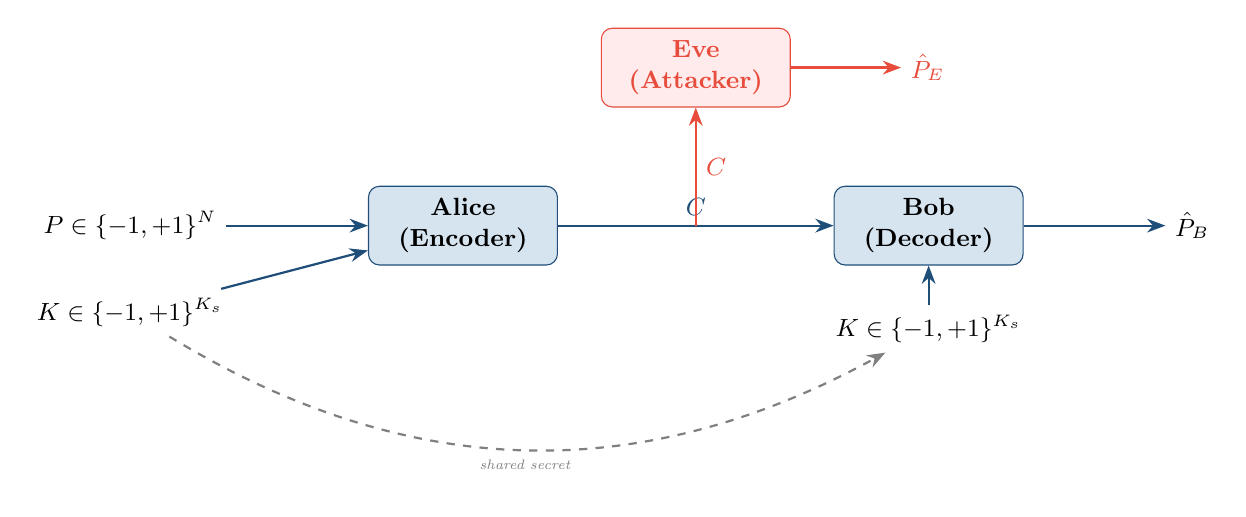
\begin{tikzpicture}[
  node distance = 1.8cm and 3.0cm,
  box/.style    = {draw=NavyBlue, fill=LightBlue, rounded corners=4pt,
                   minimum width=2.4cm, minimum height=1.0cm,
                   font=\bfseries\small, align=center},
  ebox/.style   = {draw=RedWarn,  fill=red!8,    rounded corners=4pt,
                   minimum width=2.4cm, minimum height=1.0cm,
                   font=\bfseries\small, align=center, text=RedWarn},
  arr/.style    = {-Stealth, thick, NavyBlue},
  earr/.style   = {-Stealth, thick, RedWarn},
  lbl/.style    = {font=\small\itshape, NavyBlue},
  elbl/.style   = {font=\small\itshape, RedWarn},
]
\node[box]  (alice) {\alice{}\\(Encoder)};
\node[box,  right=3.5cm of alice]  (bob)  {\bob{}\\(Decoder)};
\node[ebox, above=1.5cm of $(alice)!0.5!(bob)$] (eve) {\eve{}\\(Attacker)};
\node[left=1.8cm of alice, font=\small]         (P)   {$P \in \{-1,+1\}^N$};
\node[below=0.5cm of P,    font=\small]         (K1)  {$K \in \{-1,+1\}^{K_s}$};
\node[right=1.8cm of bob,  font=\small]         (Pb)  {$\hat{P}_B$};
\node[right=1.4cm of eve,  font=\small, RedWarn](Pe)  {$\hat{P}_E$};
\node[below=0.5cm of bob,  font=\small]         (K2)  {$K \in \{-1,+1\}^{K_s}$};
\draw[arr]  (P)  -- (alice);
\draw[arr]  (K1) -- (alice);
\draw[arr]  (alice) -- node[lbl, above]{$C$} (bob);
\draw[arr]  (bob)   -- (Pb);
\draw[arr]  (K2)    -- (bob);
\draw[earr] ($(alice)!0.5!(bob)$) -- node[elbl, right]{$C$} (eve);
\draw[earr] (eve)   -- (Pe);
\draw[arr, dashed, gray] (K1) to[bend right=30]
  node[below, font=\tiny\itshape, gray]{shared secret} (K2);
\end{tikzpicture}
\caption{Information flow in the Alice--Bob--Eve framework.
\alice{} encrypts plaintext $P$ using shared key $K$, producing ciphertext $C$.
\bob{} decrypts $C$ using the same key to recover $\hat{P}_B \approx P$.
\eve{} observes $C$ only and attempts to recover $\hat{P}_E \approx P$
without access to $K$.}
\label{fig:abe_tikz}
\end{figure}

\subsubsection*{Roles and Information Access}

The information available to each agent is summarised in
Table~\ref{tab:agent_access}. The structural asymmetry between \bob{}
(who has the key) and \eve{} (who does not) is the source of the
security advantage: any cipher that effectively uses the key will be
harder for \eve{} to break, since her network must operate without
that crucial information.

\begin{table}[H]
  \centering
  \caption{Information access for each agent in the system.}
  \label{tab:agent_access}
  \renewcommand{\arraystretch}{1.3}
  \begin{tabularx}{\linewidth}{@{} l X X X c @{}}
    \toprule
    \textbf{Agent} & \textbf{Input} & \textbf{Output} &
    \textbf{Objective} & \textbf{Has Key?} \\
    \midrule
    \alice{} & $P$, $K$ & $C$ (ciphertext)
      & Encrypt so \bob{} can decode but \eve{} cannot & \checkmark \\[4pt]
    \bob{}   & $C$, $K$ & $\hat{P}_B$ (decrypted)
      & Reconstruct $P$ accurately & \checkmark \\[4pt]
    \eve{}   & $C$ only & $\hat{P}_E$ (guessed)
      & Reconstruct $P$ from ciphertext alone & \texttimes \\
    \bottomrule
  \end{tabularx}
\end{table}

\subsubsection*{Threat Model}

The adversary \eve{} is modelled as a \textbf{passive, ciphertext-only
attacker}: she observes every ciphertext transmitted by \alice{} but
cannot intercept, modify, or replay messages, and has no access to the
shared key. This is the weakest standard threat model in cryptography.
It corresponds directly to the system architecture, where \eve{}'s
network receives only the ciphertext tensor as input:

\begin{lstlisting}[caption={Agent input construction in \code{train\_alice\_bob()}}]
cipher  = alice(tf.concat([o_msg, key], axis=1))  # Alice: [P || K]
dec_bob = bob(tf.concat([cipher, key], axis=1))   # Bob:   [C || K]
dec_eve = eve(cipher)                              # Eve:    C only
\end{lstlisting}

The assumption of one fresh key $K$ per plaintext $P$ means that
\eve{} cannot accumulate statistics across messages encrypted under
the same key --- each observation is independent. This mimics a
one-time-pad key schedule, the strongest possible key usage regime.

% =============================================================================
\subsection{The Mix-and-Transform Architecture}
\label{subsec:mix_transform}
% =============================================================================

\subsubsection*{Design Philosophy}

The architecture follows the \textbf{mix~\&~transform} design principle
introduced in~\cite{abadi2016learning}. The four central design goals are:

\begin{enumerate}[leftmargin=2em, itemsep=4pt]
  \item \textbf{Expressiveness}: must be capable of representing mixing
        functions such as XOR, without hard-coding any particular function.
  \item \textbf{Learned locality}: which bit positions to combine should
        be a \emph{learned} property, not pre-specified by the architecture.
  \item \textbf{Key exploitation}: key bits must be able to influence every
        output bit, enabling key-dependent encryption to emerge naturally.
  \item \textbf{Output range}: the final output must lie in $[-1,+1]$
        to be comparable with the binary input representation.
\end{enumerate}

These goals motivate the specific sequence: one FC layer for global
mixing, followed by four 1D convolutional layers for local transformation,
with sigmoid activations on all intermediate layers and tanh on the final
output layer.

\subsubsection*{Complete Architecture Diagram}

\begin{figure}[H]
\centering
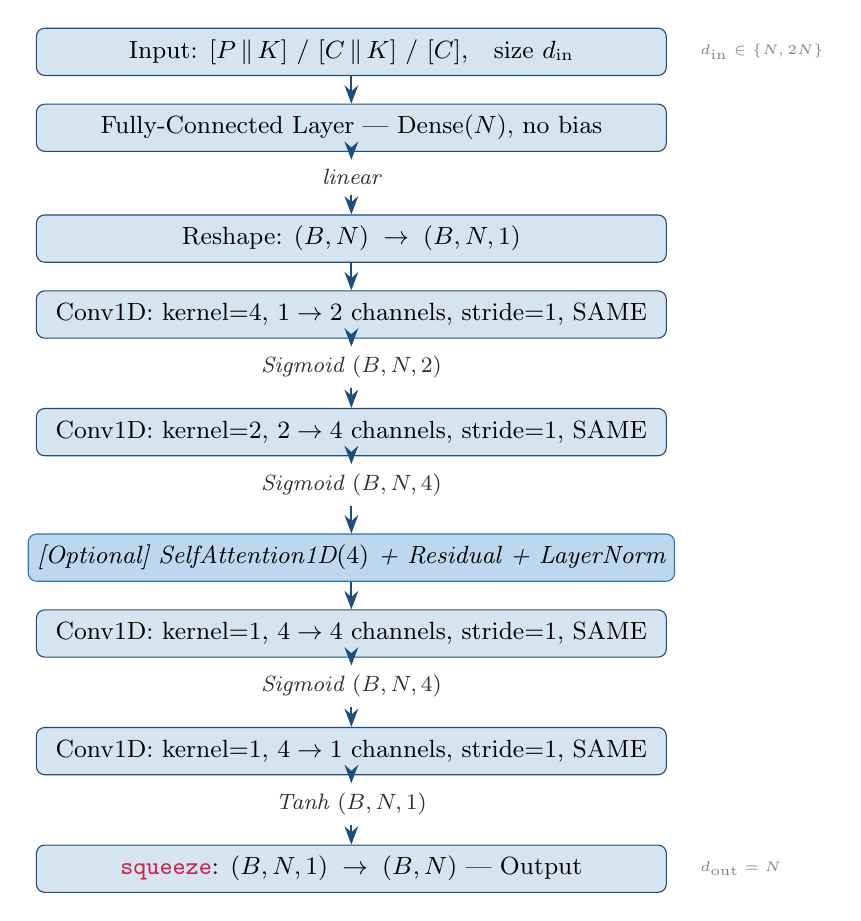
\begin{tikzpicture}[
  node distance = 0.15cm,
  layer/.style  = {draw=NavyBlue, fill=LightBlue, rounded corners=3pt,
                   minimum width=8cm, minimum height=0.6cm,
                   font=\small, align=center},
  attn/.style   = {draw=SteelBlue, fill=MidBlue, rounded corners=3pt,
                   minimum width=8cm, minimum height=0.6cm,
                   font=\small\itshape, align=center},
  act/.style    = {draw=none, fill=none, font=\footnotesize\itshape,
                   text=DarkGray, minimum height=0.35cm},
  arr/.style    = {-Stealth, NavyBlue, thick},
]
\node[layer] (inp)  {Input: $[P\,\|\,K]$ / $[C\,\|\,K]$ / $[C]$,\quad size $d_{\mathrm{in}}$};
\node[layer, below=0.35cm of inp]  (fc)   {Fully-Connected Layer --- Dense$(N)$, no bias};
\node[act,   below=0.1cm  of fc]   (a0)   {linear};
\node[layer, below=0.25cm of a0]   (rs)   {Reshape: $(B,N)\;\to\;(B,N,1)$};
\node[layer, below=0.35cm of rs]   (c1)   {Conv1D: kernel=4,\ $1\to2$ channels,\ stride=1,\ SAME};
\node[act,   below=0.1cm  of c1]   (a1)   {Sigmoid\ $(B,N,2)$};
\node[layer, below=0.25cm of a1]   (c2)   {Conv1D: kernel=2,\ $2\to4$ channels,\ stride=1,\ SAME};
\node[act,   below=0.1cm  of c2]   (a2)   {Sigmoid\ $(B,N,4)$};
\node[attn,  below=0.35cm of a2]   (att)  {\textit{[Optional]}\ SelfAttention1D$(4)$ + Residual + LayerNorm};
\node[layer, below=0.35cm of att]  (c3)   {Conv1D: kernel=1,\ $4\to4$ channels,\ stride=1,\ SAME};
\node[act,   below=0.1cm  of c3]   (a3)   {Sigmoid\ $(B,N,4)$};
\node[layer, below=0.25cm of a3]   (c4)   {Conv1D: kernel=1,\ $4\to1$ channels,\ stride=1,\ SAME};
\node[act,   below=0.1cm  of c4]   (a4)   {Tanh\ $(B,N,1)$};
\node[layer, below=0.25cm of a4]   (out)  {\code{squeeze}: $(B,N,1)\;\to\;(B,N)$ --- Output};
\foreach \x/\y in {inp/fc,fc/a0,a0/rs,rs/c1,c1/a1,a1/c2,c2/a2,
                    a2/att,att/c3,c3/a3,a3/c4,c4/a4,a4/out}
  \draw[arr] (\x) -- (\y);
\node[right=0.3cm of inp, font=\tiny, gray] {$d_{\mathrm{in}}\in\{N,2N\}$};
\node[right=0.3cm of out, font=\tiny, gray] {$d_{\mathrm{out}}=N$};
\end{tikzpicture}
\caption{Complete mix~\&~transform architecture for \code{CipherNet}
(\alice{} and \bob{}) and \code{AttackerNet} (\eve{}).
The optional self-attention block is active only when \code{--attention} is set.
Tensor shapes shown for $N=16$.}
\label{fig:arch_full}
\end{figure}

% =============================================================================
\subsection{Alice's Network: \texttt{CipherNet} (Encoder)}
\label{subsec:alice_net}
% =============================================================================

\alice{}'s network implements the encryption function
$C = f_{\thetaA}(P, K)$. Its input is the concatenation of the plaintext
$P \in \{-1,+1\}^N$ and the key $K \in \{-1,+1\}^{K_s}$, giving an input
vector of size $N + K_s = 32$ for the default configuration ($N = K_s = 16$).

\subsubsection*{FC Layer: Global Mixing}

The FC layer maps the $(N+K_s)$-dimensional input to an $N$-dimensional
representation. With no bias, the transformation is purely linear:
%
\begin{equation}
  \mathbf{h}^{(0)} \;=\; W_{\mathrm{fc}}\,[P \,\|\, K]^\top,
  \qquad W_{\mathrm{fc}} \in \mathbb{R}^{N \times (N+K_s)}
  \label{eq:alice_fc}
\end{equation}
%
This layer has $N \times (N + K_s) = 16 \times 32 = 512$ parameters.
Because every output neuron receives contributions from all 32 input units,
this layer can implement any linear mixing of plaintext and key bits ---
including pure XOR when $N = K_s$, which corresponds to $W_{\mathrm{fc}}$
being an identity-like matrix that pairs each plaintext bit with its
corresponding key bit.

\subsubsection*{Convolutional Processing}

After the FC layer the output is reshaped to $(B, N, 1)$ to create a
single-channel 1D sequence of length $N$. The four convolutional layers
then progressively transform this sequence:

\begin{itemize}[leftmargin=1.8em, itemsep=4pt]
  \item \textbf{Conv1} (kernel=4, $1\to2$ ch, stride=1): slides a
        width-4 window, capturing short-range interactions between
        adjacent positions in the mixed representation.
  \item \textbf{Conv2} (kernel=2, $2\to4$ ch, stride=1): expands
        the channel depth to four while preserving sequence length at $N=16$.
        The kernel-2 window captures pairwise interactions between adjacent positions.
  \item \textbf{Conv3} (kernel=1, $4\to4$ ch, stride=1): applies an
        independent pointwise transformation to each position ---
        equivalent to a per-position FC layer across the channel dimension.
  \item \textbf{Conv4} (kernel=1, $4\to1$ ch, stride=1): reduces to a
        single channel. The tanh activation constrains outputs to
        $(-1,+1)$, producing the ciphertext $C$.
\end{itemize}

\subsubsection*{Parameter Count}

\begin{table}[H]
  \centering
  \caption{Parameter count for \alice{}'s \code{CipherNet}
           ($N=16$, $K_s=16$, no attention).}
  \label{tab:alice_params}
  \renewcommand{\arraystretch}{1.25}
  \begin{tabular}{@{} l r r r @{}}
    \toprule
    \textbf{Layer} & \textbf{Shape} & \textbf{Parameters} & \textbf{Activation} \\
    \midrule
    FC (Dense)  & $32 \to 16$             & 512 & Linear  \\
    Conv1       & $4\!\times\!1\!\times\!2 + 2$ & 10 & Sigmoid \\
    Conv2       & $2\!\times\!2\!\times\!4 + 4$ & 20 & Sigmoid \\
    Conv3       & $1\!\times\!4\!\times\!4 + 4$ & 20 & Sigmoid \\
    Conv4       & $1\!\times\!4\!\times\!1 + 1$ & 5  & Tanh    \\
    \midrule
    \textbf{Total} & & \textbf{567} & \\
    \bottomrule
  \end{tabular}
\end{table}

Alice's network has only \textbf{567 parameters} (512 FC weights plus
55 conv weights and biases) --- an intentionally lightweight architecture
that ensures emergent encryption arises from genuine learning, not from
excessive model capacity. Note that only the FC layer sets
\code{use\_bias=False}; all four Conv1D layers retain their default
Keras bias terms.

% =============================================================================
\subsection{Bob's Network: \texttt{CipherNet} (Decoder)}
\label{subsec:bob_net}
% =============================================================================

\bob{}'s network implements the decryption function
$\hat{P}_B = g_{\thetaB}(C, K)$. It is \textbf{architecturally identical}
to \alice{}'s network --- the same \code{CipherNet} class is instantiated
twice --- but its input is the concatenation of the \emph{ciphertext} $C$
and the shared key $K$:

\begin{lstlisting}[caption={Bob's input: ciphertext concatenated with the shared key}]
dec_bob = bob(tf.concat([cipher, key], axis=1))
# Shape: (B, N + key_size) = (B, 32)
\end{lstlisting}

\subsubsection*{Shared Architecture, Independent Weights}

Although \alice{} and \bob{} share the same \code{CipherNet} architecture,
they are \textbf{separate Keras model instances} with entirely independent
weight tensors $\thetaA \neq \thetaB$. Encryption and decryption need not
be the same function. Both $\thetaA$ and $\thetaB$ are updated jointly in
each Alice/Bob training step, since the composite loss depends on both:

\begin{lstlisting}[caption={Joint update of Alice and Bob parameters}]
grads = tape.gradient(loss,
    alice.trainable_variables + bob.trainable_variables)
optimizer_ab.apply_gradients(
    zip(grads, alice.trainable_variables + bob.trainable_variables))
\end{lstlisting}

This joint optimisation is what enables co-development of a shared
protocol: neither can succeed in isolation, and both are updated to
maximise their mutual benefit.

% =============================================================================
\subsection{Eve's Network: \texttt{AttackerNet}}
\label{subsec:eve_net}
% =============================================================================

\eve{}'s network implements $\hat{P}_E = h_{\thetaE}(C)$. It uses the
\code{AttackerNet} class, which has \textbf{identical internal architecture}
to \code{CipherNet} (FC $+$ 4 convolutions $+$ same activations), but
differs in two critical respects.

\subsubsection*{Structural Disadvantage: No Key Access}

\eve{} receives only the ciphertext $C$ as input. Her input size is $N=16$,
not $N+K_s=32$. Her FC layer is therefore a $16\times16=256$ parameter
matrix, compared to Alice's $32\times16=512$. The reduced input dimension
is the primary source of difficulty: any encryption that effectively uses
$K$ creates a family of $2^{K_s}$ possible ciphertexts for each plaintext,
and \eve{} cannot distinguish between them without knowing the key.

\begin{table}[H]
  \centering
  \caption{Structural comparison: \code{CipherNet} vs.\ \code{AttackerNet}.}
  \label{tab:net_comparison}
  \renewcommand{\arraystretch}{1.25}
  \begin{tabular}{@{} l c c @{}}
    \toprule
    \textbf{Component} & \textbf{CipherNet} (\alice{}/\bob{}) &
    \textbf{AttackerNet} (\eve{}) \\
    \midrule
    Input size    & $N + K_s = 32$  & $N = 16$     \\
    FC layer      & $32 \to 16$     & $16 \to 16$  \\
    FC parameters & $512$           & $256$        \\
    Conv layers   & identical       & identical    \\
    Total params  & $567$           & $311$        \\
    Key access    & \checkmark      & \texttimes   \\
    \bottomrule
  \end{tabular}
\end{table}

\subsubsection*{Independent Optimisation}

\eve{}'s parameters $\thetaE$ are updated using a fully separate Adam
optimiser instance \code{opt\_eve}. This decoupling is essential: if
\eve{} were updated jointly with \alice{} and \bob{}, no genuine
adversarial pressure would exist. The two optimisation problems must
remain independent:

\begin{lstlisting}[caption={Separate independent optimisers}]
opt_ab  = keras.optimizers.Adam(args.lr)  # for Alice + Bob
opt_eve = keras.optimizers.Adam(args.lr)  # for Eve -- fully independent
\end{lstlisting}

% =============================================================================
\subsection{Data Representation}
\label{subsec:data_repr}
% =============================================================================

\subsubsection*{Binary Encoding: $\{-1,+1\}$ vs.\ $\{0,1\}$}

The system uses $\{-1,+1\}$ rather than $\{0,1\}$ as the binary
representation. In $\{-1,+1\}$ space, the XOR operation corresponds to
\emph{multiplication}:
%
\begin{equation}
  a \oplus b \;\;\longleftrightarrow\;\; a \cdot b,
  \qquad a, b \in \{-1,+1\}
  \label{eq:xor_mult}
\end{equation}
%
Multiplication is differentiable, making XOR-like interactions expressible
by smooth neural network computations. In $\{0,1\}$ space, XOR has no
smooth algebraic analogue, making it harder for gradient descent to discover.

\subsubsection*{Floating-Point Ciphertext}

While plaintexts and keys are constrained to $\{-1,+1\}^N$, the ciphertext
$C$ is a vector of \emph{real-valued} floating-point numbers in $(-1,+1)$
enforced by the tanh output. This continuous ciphertext space allows
gradient information to flow smoothly from \eve{}'s loss back through
the ciphertext to \alice{}'s parameters, enabling end-to-end training.
Without this continuity, gradient-based optimisation of \alice{} would
not be possible.

% =============================================================================
\newpage
\section{Loss Functions \& Optimisation Objectives}
\label{sec:loss}
% =============================================================================

The loss functions are the heart of the adversarial neural cryptography
system. They encode the security objectives, determine what each agent
learns, and govern the competitive dynamics of training. This section
formally derives each loss, analyses the design choices behind them, and
compares the three variants implemented in \code{main\_enhanced.py}.

% =============================================================================
\subsection{The L1 Distance Function}
\label{subsec:l1}
% =============================================================================

All loss functions in this system are built on the \textbf{L1 distance}:
%
\begin{equation}
  d_1(\mathbf{a},\, \mathbf{b})
  \;=\; \|\mathbf{a} - \mathbf{b}\|_1
  \;=\; \sum_{i=1}^{N} |a_i - b_i|
  \label{eq:l1_full}
\end{equation}

\begin{lstlisting}[caption={L1 distance implementation}]
def l1_distance(a, b):
    return tf.reduce_sum(tf.abs(a - b), axis=1)
    # shape (B,) -- one scalar per batch element
\end{lstlisting}

\subsubsection*{Why L1 and Not L2?}

For binary $\{-1,+1\}$ signals, L1 distance has a direct interpretation.
If $a_i, b_i \in \{-1,+1\}$, then $|a_i - b_i| \in \{0, 2\}$: it is $0$
when bits agree and $2$ when they differ. Therefore $d_1(P, \hat{P})/2$
counts the exact \emph{number of bit errors}. For $N=16$, the maximum L1
distance is $32$ (all bits wrong) and the random-guessing baseline is $16$
(8 bits wrong $\times$ 2). L2 distance squares the errors, making large
individual errors dominate and losing the clean bit-counting interpretation.

% =============================================================================
\subsection{Eve's Loss Function}
\label{subsec:eve_loss}
% =============================================================================

\eve{}'s objective is to reconstruct $P$ from $C$ alone. Her per-example
loss is the L1 distance between her reconstruction and the true plaintext:
%
\begin{equation}
  \ell_E(\thetaA, \thetaE,\, P, K)
  \;=\; d_1\!\left(P,\; h_{\thetaE}\!\left(f_{\thetaA}(P,K)\right)\right)
  \label{eq:eve_loss_formal}
\end{equation}
%
The batch loss minimised during training is the mean over the batch $B$:
%
\begin{equation}
  \mathcal{L}_E(\thetaA, \thetaE)
  \;=\; \frac{1}{B} \sum_{b=1}^{B}
        d_1\!\left(P^{(b)},\; h_{\thetaE}\!\left(C^{(b)}\right)\right)
  \label{eq:eve_loss_batch}
\end{equation}

\begin{lstlisting}[caption={Eve's loss and isolated training step}]
def eve_loss(o_message, decipher_eve):
    return tf.reduce_mean(l1_distance(o_message, decipher_eve))

@tf.function
def train_eve(alice, eve, o_msg, key, optimizer_eve):
    with tf.GradientTape() as tape:
        cipher  = alice(tf.concat([o_msg, key], axis=1))
        dec_eve = eve(cipher)
        loss    = eve_loss(o_msg, dec_eve)
    grads = tape.gradient(loss, eve.trainable_variables)
    optimizer_eve.apply_gradients(
        zip(grads, eve.trainable_variables))
    return loss, dec_eve
\end{lstlisting}

Note that \alice{}'s parameters receive \textbf{no gradient updates} in
this step: the tape is scoped to \code{eve.trainable\_variables} only.
\alice{}'s forward pass is included solely to generate the ciphertext.

% =============================================================================
\subsection{Alice and Bob's Composite Loss}
\label{subsec:ab_loss}
% =============================================================================

\alice{} and \bob{}'s loss simultaneously encourages two competing goals:
accurate reconstruction by \bob{} and adversarial confusion for \eve{}.
These are combined additively:
%
\begin{equation}
  \mathcal{L}_{AB}(\thetaA, \thetaB)
  \;=\;
  \underbrace{
    \frac{1}{B}\sum_{b=1}^B
    \frac{d_1(P^{(b)},\, \hat{P}_B^{(b)})}{N}
  }_{\text{Bob's reconstruction term}}
  \;+\;
  \underbrace{
    \frac{1}{B}\sum_{b=1}^B
    \mathcal{L}_{\mathrm{adv}}(P^{(b)},\, \hat{P}_E^{(b)})
  }_{\text{Adversarial penalty on Eve}}
  \label{eq:ab_loss_full}
\end{equation}

\begin{lstlisting}[caption={Alice and Bob's composite loss function}]
def alice_bob_loss(o_message, decipher_bob, decipher_eve,
                   msg_size, variant="quadratic"):
    bob_err     = l1_distance(o_message, decipher_bob) / msg_size
    adv_penalty = eve_adversarial_loss(
                      o_message, decipher_eve, msg_size, variant)
    return tf.reduce_mean(bob_err + adv_penalty)
\end{lstlisting}

\subsubsection*{Normalisation of Bob's Error Term}

Bob's reconstruction error is divided by $N$ before being added to the
adversarial penalty. This normalisation ensures both terms are on a
comparable scale: Bob's normalised L1 error lies in $[0, 2]$, and all
adversarial penalty variants also lie in $[0, 1]$ or close to it.
Without normalisation, Bob's raw error (up to $2N = 32$) would dominate
the adversarial term and the system would focus entirely on reconstruction,
neglecting security objectives.

% =============================================================================
\subsection{The Adversarial Penalty: Three Variants}
\label{subsec:adv_penalty}
% =============================================================================

The adversarial penalty $\mathcal{L}_{\mathrm{adv}}$ encodes the goal
of keeping \eve{} at the random-guessing baseline. All three variants
share the same fundamental target: \eve{}'s L1 error should equal $N/2$
in expectation. This target is \textbf{not the maximum possible error}:
if \alice{} and \bob{} drove \eve{}'s error to the maximum of $2N$
(all bits wrong), \eve{} could negate her output and achieve zero error.
Targeting $N/2$ ensures \eve{}'s output is maximally \emph{uninformative}.

\subsubsection*{Variant 1: Quadratic Penalty}

\begin{equation}
  \boxed{
  \mathcal{L}_{\mathrm{adv}}^{\mathrm{quad}}
  \;=\;
  \frac{\Bigl(\dfrac{N}{2} - d_1(P,\, \hat{P}_E)\Bigr)^2}
       {\Bigl(\dfrac{N}{2}\Bigr)^2}
  }
  \label{eq:adv_quad}
\end{equation}

This is the original formulation from~\cite{abadi2016learning}. The
quadratic form is minimised at $d_1 = N/2$ and grows symmetrically
on both sides, penalising both $d_1 < N/2$ (Eve does better than
random) and $d_1 > N/2$ (Eve does worse --- undesirable since she
can trivially reverse the cipher). The gradient:
%
\begin{equation}
  \frac{\partial \mathcal{L}_{\mathrm{adv}}^{\mathrm{quad}}}{\partial d_1}
  \;=\; \frac{-2\bigl(\tfrac{N}{2} - d_1\bigr)}{\bigl(\tfrac{N}{2}\bigr)^2}
  \label{eq:quad_grad}
\end{equation}
%
grows linearly as \eve{}'s error diverges from the target, applying
fine-grained control near $N/2$ and stronger pressure far from it.

\subsubsection*{Variant 2: Linear Penalty}

\begin{equation}
  \mathcal{L}_{\mathrm{adv}}^{\mathrm{lin}}
  \;=\;
  \frac{\max\!\left(0,\;\dfrac{N}{2} - d_1(P,\, \hat{P}_E)\right)}
       {\dfrac{N}{2}}
  \label{eq:adv_linear}
\end{equation}

The linear variant applies a penalty only when \eve{} performs
\emph{better} than random guessing ($d_1 < N/2$). When $d_1 \geq N/2$,
the penalty is zero. The constant gradient $-1/(N/2)$ regardless of
distance from the target makes this variant coarser than the quadratic
near $N/2$, leading to oscillation and reduced training stability.

\subsubsection*{Variant 3: Binary Cross-Entropy Penalty}

\begin{equation}
  \mathcal{L}_{\mathrm{adv}}^{\mathrm{bce}}
  \;=\;
  -\frac{1}{N}\sum_{i=1}^{N}
    \Bigl[
      \tfrac{1}{2}\log \hat{p}_{E,i}
    + \tfrac{1}{2}\log(1 - \hat{p}_{E,i})
    \Bigr]
  \label{eq:adv_bce}
\end{equation}
%
where $\hat{p}_{E,i} = (\hat{P}_{E,i}+1)/2 \in [0,1]$ maps \eve{}'s
output to a probability. The target is $0.5$ --- maximum uncertainty
for a binary variable. The negative sign means \alice{} and \bob{} maximise
\eve{}'s output entropy, which is a stronger information-theoretic
condition closer to Shannon's notion of perfect secrecy~\cite{shannon1949communication}.

\begin{lstlisting}[caption={All three adversarial penalty variants}]
def eve_adversarial_loss(o_message, decipher_eve, msg_size,
                          variant="quadratic"):
    half    = msg_size / 2.0
    eve_err = l1_distance(o_message, decipher_eve)

    if variant == "quadratic":
        return tf.square(half - eve_err) / (half ** 2)
    elif variant == "linear":
        return tf.maximum(0.0, half - eve_err) / half
    elif variant == "bce":
        eve_prob = (decipher_eve + 1.0) / 2.0
        target   = tf.ones_like(eve_prob) * 0.5
        bce      = tf.reduce_mean(
            keras.losses.binary_crossentropy(target, eve_prob),
            axis=-1)
        return -bce
\end{lstlisting}

\subsubsection*{Comparison Summary}

\begin{table}[H]
  \centering
  \caption{Comparison of the three adversarial penalty variants
           implemented in \code{main\_enhanced.py}.}
  \label{tab:loss_comparison}
  \renewcommand{\arraystretch}{1.4}
  \begin{tabularx}{\linewidth}{@{} l X X X @{}}
    \toprule
    \textbf{Property} & \textbf{Quadratic} & \textbf{Linear} &
    \textbf{BCE} \\
    \midrule
    Minimised at        & $d_1 = N/2$     & $d_1 \geq N/2$  & max entropy \\
    Gradient near target & Near zero (fine) & Constant (coarse) & Output-dependent \\
    Symmetric penalty   & Yes             & No (one-sided)  & No \\
    Range               & $[0,1]$         & $[0,1]$         & Unbounded below \\
    Theoretical basis   & Empirical bit target & Empirical  & Shannon entropy \\
    Training stability  & High            & Moderate        & Moderate \\
    \bottomrule
  \end{tabularx}
\end{table}

% =============================================================================
\subsection{The Training Step Ratio}
\label{subsec:step_ratio}
% =============================================================================

A critical hyperparameter not reflected in the loss functions is the
\textbf{training step ratio}: for each Alice/Bob update, \eve{} receives
\code{args.eve\_steps} updates (default: 2). This gives \eve{} a
computational edge, approximating the ``optimal Eve'' concept without
requiring a costly inner optimisation loop.

\begin{lstlisting}[caption={Configurable training step ratio in the main loop}]
for step in range(args.steps):
    ab_loss, dec_bob, dec_eve, cipher = train_alice_bob(
        alice, bob, eve, msg, key, opt_ab, args.msg_size, args.loss_fn)
    for _ in range(args.eve_steps):       # default: 2
        msg_e, key_e = data_fn()
        eve_l, _ = train_eve(alice, eve, msg_e, key_e, opt_eve)
\end{lstlisting}

\begin{tcolorbox}[contribbox, title={Effect of the Training Step Ratio}]
\begin{itemize}[leftmargin=1em, itemsep=3pt, label=$\bullet$]
  \item \textbf{eve\_steps = 1} (balanced): \eve{} may be too weak;
        \alice{} and \bob{} may converge to trivial ciphers that do
        not generalise to a stronger attacker.
  \item \textbf{eve\_steps = 2} (default): the paper's recommended baseline.
        Achieves approximately 70\% training success rate, but
        experimentally surpassed by eve\_steps=4 (Section~\ref{sec:results}).
  \item \textbf{eve\_steps = 3--4} (stronger pressure): counter-intuitively,
        stronger adversarial pressure can \emph{improve} convergence by
        forcing Alice and Bob to develop robust key-dependent encryption
        earlier. Experimentally (Section~\ref{sec:results}), eve\_steps=4
        achieves the best result: Bob error 0.03~bits and 5/5 secure runs.
\end{itemize}
\end{tcolorbox}

% =============================================================================
\subsection{Variable Scope and Parameter Isolation}
\label{subsec:var_scope}
% =============================================================================

A subtle but essential aspect of the implementation is that \alice{}/\bob{}'s
parameters and \eve{}'s parameters must be updated \emph{independently}.
In \code{main\_enhanced.py}, this is enforced by Keras model ownership of
\code{trainable\_variables}, and by \code{tf.GradientTape} scoping:

\begin{itemize}[leftmargin=1.8em, itemsep=4pt]
  \item \code{train\_alice\_bob()}: gradients computed for
        \code{alice.trainable\_variables + bob.trainable\_variables} only.
        \eve{}'s forward pass is included to evaluate the adversarial
        loss, but her variables receive \textbf{no gradient updates}.
  \item \code{train\_eve()}: gradients computed for
        \code{eve.trainable\_variables} only.
        \alice{}'s variables receive \textbf{no gradient updates}.
\end{itemize}

The \code{@tf.function} decorator compiles both training steps into
TensorFlow graph operations, ensuring reproducible gradient flow and
eliminating Python-level overhead during the 20{,}000-step training loop.
This clean separation is what makes the adversarial dynamic genuine:
\eve{} cannot benefit from Alice and Bob's loss gradient, and
\alice{}/\bob{} cannot accidentally optimise \eve{}'s objective.


% =============================================================================
\newpage
\section{Training Dynamics \& Convergence}
\label{sec:training_dynamics}
% =============================================================================

The training of adversarial neural cryptography systems differs fundamentally
from standard supervised learning. Because three agents are optimised
simultaneously with conflicting objectives, the training dynamics are
governed by competitive co-evolution rather than simple gradient descent
on a fixed loss landscape. This section analyses the adversarial game
structure, the characteristic convergence behaviour observed in practice,
the four-phase learning trajectory, the effect of the configurable step
ratio, and the key hyperparameters that govern stability.

% =============================================================================
\subsection{Adversarial Training as a Minimax Game}
\label{subsec:minimax_game}
% =============================================================================

\subsubsection*{The Two-Level Optimisation Problem}

The full training objective can be written as a nested minimax problem.
\alice{} and \bob{} seek parameters that minimise their composite loss
against the \emph{best possible} \eve{}, while \eve{} seeks parameters
that minimise her reconstruction loss given \alice{}'s current cipher:
%
\begin{equation}
  \min_{\thetaA,\,\thetaB} \;\;
  \mathcal{L}_{AB}\!\left(
    \thetaA,\, \thetaB,\;
    \underbrace{\arg\min_{\thetaE} \mathcal{L}_E(\thetaA, \thetaE)}_{\text{optimal Eve}}
  \right)
  \label{eq:nested_minimax}
\end{equation}
%
Computing the optimal \eve{} exactly would require solving an inner
optimisation problem at every step of the outer loop --- a procedure
equivalent to the original GAN training derivation of Goodfellow et
al.~\cite{goodfellow2014generative}, which is computationally intractable.
The practical approximation used in \code{main\_enhanced.py} is to perform
\code{args.eve\_steps} gradient steps on \eve{} for every one gradient step
on \alice{} and \bob{}, maintaining a moving approximation to the optimal
\eve{} throughout training.

\subsubsection*{Saddle-Point Nature of the Optimisation}

The equilibrium of the adversarial game is a \textbf{saddle point} of the
joint objective --- a point $(\thetaA^*, \thetaB^*, \thetaE^*)$ where:
%
\begin{align}
  \mathcal{L}_{AB}(\thetaA^*, \thetaB^*, \thetaE^*)
    &\leq \mathcal{L}_{AB}(\thetaA, \thetaB, \thetaE^*)
    \quad \forall\; \thetaA, \thetaB
    \label{eq:saddle_ab} \\[4pt]
  \mathcal{L}_E(\thetaA^*, \thetaE^*)
    &\leq \mathcal{L}_E(\thetaA^*, \thetaE)
    \quad \forall\; \thetaE
    \label{eq:saddle_e}
\end{align}
%
At this saddle point, \bob{}'s reconstruction error is near zero,
\eve{}'s reconstruction error is near $N/2$, and no agent can
improve its outcome by unilaterally changing its parameters.

Unlike standard convex optimisation, saddle-point problems have no
guarantee of convergence under simultaneous gradient descent. The
loss landscape of each agent changes as the others update their
parameters, creating a moving target for every gradient step. This
is why adversarial training exhibits the oscillatory, non-monotonic
behaviour described in the next subsection.

\subsubsection*{Existence and Uniqueness of the Equilibrium}

In the neural cryptography setting, the existence of a Nash equilibrium
is not guaranteed in general, because the loss functions are non-convex
in the network parameters. However, Abadi and
Andersen~\cite{abadi2016learning} demonstrate empirically that a
meaningful equilibrium is reached in a significant fraction of training
runs (approximately 14 out of 20 for $N=16$). The system's design ---
particularly the use of a small, symmetric architecture and a learning
rate that is not decayed --- increases the probability of reaching
such an equilibrium.

% =============================================================================
\subsection{The Four Phases of Training}
\label{subsec:four_phases}
% =============================================================================

Across successful training runs, the loss curves produced by
\code{save\_loss\_curves()} in \code{main\_enhanced.py} exhibit a
characteristic four-phase trajectory. Understanding these phases is
essential for interpreting experimental results and diagnosing
training failures.

\begin{figure}[H]
\centering
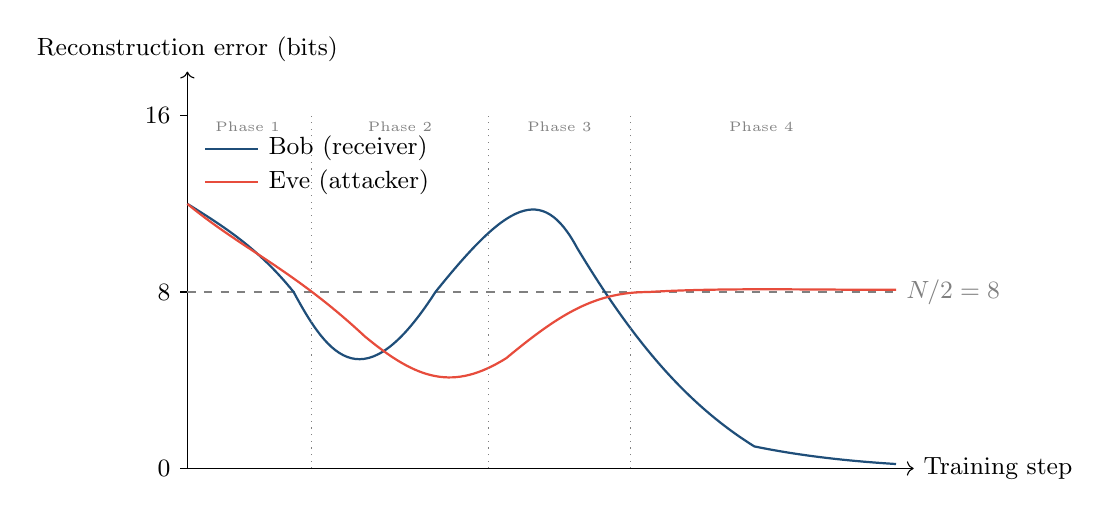
\begin{tikzpicture}[
  x=0.045cm, y=0.28cm,
  every node/.style={font=\small},
]
% Axes
\draw[->] (0,0) -- (205,0) node[right] {Training step};
\draw[->] (0,0) -- (0,18)  node[above] {Reconstruction error (bits)};

% Y-axis ticks
\foreach \y/\lbl in {0/0, 8/8, 16/16} {
  \draw (-2,\y) -- (0,\y);
  \node[left] at (-2,\y) {\lbl};
}

% Random baseline
\draw[dashed, gray, thick] (0,8) -- (200,8)
  node[right, gray] {$N/2 = 8$};

% Bob's error curve (rough piecewise approximation)
\draw[NavyBlue, thick]
  (0,12) .. controls (10,11) and (20,10) .. (30,8)
         .. controls (40,5)  and (50,3)  .. (70,8)
         .. controls (90,12) and (100,13).. (110,10)
         .. controls (125,6) and (140,3) .. (160,1)
         .. controls (175,0.5) and (190,0.3)..(200,0.2);

% Eve's error curve
\draw[RedWarn, thick]
  (0,12) .. controls (15,10) and (30,9)  .. (50,6)
         .. controls (65,4)  and (75,3.5).. (90,5)
         .. controls (105,7) and (115,8) .. (130,8)
         .. controls (150,8.2) and (175,8.1)..(200,8.1);

% Phase separators
\foreach \x in {35, 85, 125}
  \draw[dotted, gray] (\x,0) -- (\x,16);

% Phase labels
\node[align=center, gray] at (17,15.5) {\tiny Phase 1};
\node[align=center, gray] at (60,15.5) {\tiny Phase 2};
\node[align=center, gray] at (105,15.5){\tiny Phase 3};
\node[align=center, gray] at (162,15.5){\tiny Phase 4};

% Legend
\draw[NavyBlue, thick] (5,14.5) -- (20,14.5)
  node[right, black] {\small Bob (receiver)};
\draw[RedWarn, thick]  (5,13.0) -- (20,13.0)
  node[right, black] {\small Eve (attacker)};

\end{tikzpicture}
\caption{Schematic of the four-phase training trajectory observed in
successful runs. Bob's error (blue) eventually converges near zero;
Eve's error (red) converges near the random-guessing baseline of $N/2=8$.
The non-monotonic behaviour between Phases~2 and~3 is characteristic
of adversarial training dynamics.}
\label{fig:four_phases}
\end{figure}

\subsubsection*{Phase 1 --- Random Exploration (Steps 0--$\sim$500)}

In the initial phase, all three networks have random weights and produce
essentially random outputs. Both \bob{}'s and \eve{}'s reconstruction
errors are close to the random-guessing baseline of $N/2$, since neither
can decode anything meaningful. The gradients from $\mathcal{L}_{AB}$
begin to push \alice{} and \bob{} toward finding any communication
protocol, regardless of security. \eve{}'s gradients push her to exploit
whatever structure emerges.

\subsubsection*{Phase 2 --- Trivial Cipher Discovery (Steps $\sim$500--$\sim$3000)}

\alice{} and \bob{} discover a simple communication protocol, potentially
similar to an identity mapping or a simple linear transform. \bob{}'s
error begins to drop sharply, indicating successful communication. However,
this early cipher makes little use of the key $K$ --- the ciphertext is
largely predictable from the plaintext alone --- so \eve{} can also
begin to exploit the structure. \eve{}'s error drops below the
random-guessing baseline.

\subsubsection*{Phase 3 --- Eve Breaks the Trivial Cipher (Steps $\sim$3000--$\sim$8000)}

\eve{}'s continued gradient updates allow her to adapt to \alice{}'s
simple cipher, reducing her reconstruction error significantly. This
creates a crisis for \alice{} and \bob{}: their composite loss
$\mathcal{L}_{AB}$ increases because the adversarial penalty
$\mathcal{L}_{\mathrm{adv}}$ grows as \eve{} improves. This is the
most critical and potentially unstable phase of training. Two outcomes
are possible:

\begin{itemize}[leftmargin=1.8em, itemsep=4pt]
  \item \textbf{Successful adaptation}: \alice{} and \bob{} feel the
        gradient pressure from the growing adversarial penalty and begin
        discovering key-dependent encryption strategies. The system
        progresses to Phase~4.
  \item \textbf{Training failure}: \alice{} and \bob{} fail to discover
        a better cipher within the training budget, and the system
        oscillates or stagnates. This accounts for approximately 30\%
        of training runs for $N=16$.
\end{itemize}

\subsubsection*{Phase 4 --- Key-Exploiting Encryption (Steps $\sim$8000--20000)}

In successful runs, \alice{} and \bob{} discover encryption strategies
that effectively use the shared key $K$. Because \eve{} does not have
access to $K$, she can no longer decode the ciphertext --- her error
rises back toward and stabilises near the random-guessing baseline of
$N/2$. Meanwhile, \bob{}'s error continues to decrease toward zero,
since he has $K$ and can invert \alice{}'s key-dependent transformation.
This phase corresponds to the genuine emergence of symmetric encryption
as a learned behaviour.

The progression through these phases is directly observable in the
loss-curve plots generated by \code{save\_loss\_curves()} in
\code{main\_enhanced.py}, which saves a \texttt{.png} figure of Bob's
and Eve's errors versus training step to the \code{--plot\_dir} directory.

% =============================================================================
\subsection{Non-Monotonic Convergence Behaviour}
\label{subsec:nonmonotonic}
% =============================================================================

A defining characteristic of adversarial training that distinguishes
it from standard supervised learning is its \textbf{non-monotonic
convergence}. In supervised learning, the training loss is expected
to decrease (or at least not increase significantly) at each gradient
step, because the loss landscape is fixed. In adversarial training,
the loss landscape for each agent \emph{changes} as the other agents
update, producing the following non-monotonic phenomena:

\begin{enumerate}[leftmargin=2em, itemsep=5pt]

  \item \textbf{Bob's error temporarily increases (Phase~3)}: when
        \alice{} and \bob{} abandon their trivial cipher and begin
        searching for a key-dependent one, \bob{}'s reconstruction error
        may temporarily rise. This is not a sign of divergence, but of
        the system exploring a new region of parameter space.

  \item \textbf{Eve's error oscillates}: as \alice{}'s encryption
        strategy changes, the ciphertext distribution changes, causing
        \eve{}'s error to fluctuate. \eve{} must continuously adapt to
        a moving target.

  \item \textbf{Multiple restarts possible}: the system can visit
        the trivial-cipher regime multiple times before settling on
        a secure cipher, particularly when the training step ratio
        is not well-calibrated.

\end{enumerate}

\noindent This behaviour is expected and theoretically grounded: it is
the neural analogue of the arms-race dynamics observed in evolutionary
biology and game theory. The key practical implication is that
\textbf{early stopping based on the loss is inappropriate} for this
system --- a temporarily high loss does not indicate that training should
be terminated. The full 20{,}000 step budget is generally required.

% =============================================================================
\subsection{Hyperparameter Sensitivity}
\label{subsec:hyperparams}
% =============================================================================

The system's training dynamics are sensitive to several hyperparameters.
Table~\ref{tab:hyperparams} summarises the key parameters, their default
values in \code{main\_enhanced.py}, and their effect on convergence.

\begin{table}[H]
  \centering
  \caption{Key hyperparameters and their effect on training dynamics.}
  \label{tab:hyperparams}
  \renewcommand{\arraystretch}{1.4}
  \begin{tabularx}{\linewidth}{@{} l c X @{}}
    \toprule
    \textbf{Hyperparameter} & \textbf{Default} & \textbf{Effect on Convergence} \\
    \midrule
    Learning rate $\alpha$  & $0.0008$ &
      Slightly below the Adam default ($0.001$). Too large causes
      oscillation; too small causes slow Phase~3 transition. \\[4pt]
    Batch size $B$          & $4096$ &
      Large batches provide stable gradient estimates critical in the
      adversarial setting. Smaller batches (e.g.\ 512) reduce success
      rate significantly~\cite{abadi2016learning}. \\[4pt]
    Training steps          & $20000$ &
      Sufficient for Phase~4 to emerge in most successful runs. Fewer
      steps may terminate training during Phase~3. \\[4pt]
    Eve steps ratio         & $2$ &
      One Alice/Bob update per two Eve updates. Approximates the
      optimal Eve without an expensive inner loop. \\[4pt]
    Message size $N$        & $16$ &
      Larger $N$ increases task difficulty. $N=16$ is the standard
      benchmark from~\cite{abadi2016learning}. \\
    \bottomrule
  \end{tabularx}
\end{table}

\subsubsection*{Effect of Batch Size}

The large default batch size of $B=4096$ is particularly important
and often overlooked. In the adversarial setting, gradient estimates
must be reliable enough for each agent to detect the subtle changes
caused by the other agents' updates. With small batches (e.g.\ $B=64$),
gradient noise can completely mask the adversarial signal, causing the
system to behave as if the other agents are not adapting. The result
is that \alice{} and \bob{} converge to a trivial cipher and never
feel sufficient adversarial pressure to develop key-dependent encryption.

\subsubsection*{Effect of Message Size}

Increasing $N$ increases the task difficulty in two ways: the cipher
space grows exponentially (there are $2^N$ possible plaintexts), and
the number of parameters in the FC layer grows quadratically with $N$.
For $N=16$ (the default), the system has a high enough success rate
to study experimentally. For larger $N$, longer training runs and
potentially larger architectures are required.

% =============================================================================
\subsection{The Role of \texttt{@tf.function} in Training Speed}
\label{subsec:tf_function}
% =============================================================================

The two training step functions \code{train\_alice\_bob()} and
\code{train\_eve()} are decorated with \code{@tf.function}, which
compiles them into a TensorFlow computation graph on the first call:

\begin{lstlisting}[caption={\texttt{@tf.function} compilation of training steps}]
@tf.function
def train_alice_bob(alice, bob, eve, o_msg, key,
                    optimizer_ab, msg_size, loss_variant):
    with tf.GradientTape() as tape:
        cipher  = alice(tf.concat([o_msg, key], axis=1))
        dec_bob = bob(tf.concat([cipher, key], axis=1))
        dec_eve = eve(cipher)
        loss    = alice_bob_loss(
                      o_msg, dec_bob, dec_eve, msg_size, loss_variant)
    grads = tape.gradient(
        loss, alice.trainable_variables + bob.trainable_variables)
    optimizer_ab.apply_gradients(
        zip(grads, alice.trainable_variables + bob.trainable_variables))
    return loss, dec_bob, dec_eve, cipher
\end{lstlisting}

The \code{@tf.function} decorator offers two important benefits in the
adversarial training context:

\begin{itemize}[leftmargin=1.8em, itemsep=4pt]
  \item \textbf{Speed}: graph-mode execution eliminates Python interpreter
        overhead from the inner loop of 20{,}000 steps $\times$ 3 Eve steps
        = up to 60{,}000 total gradient computations. This typically
        provides a $3\times$ to $5\times$ speedup over eager execution
        for this architecture.
  \item \textbf{Gradient isolation}: by compiling the function into a
        fixed graph, the scope of each \code{GradientTape} is made
        explicit and reproducible, eliminating the risk of accidentally
        capturing variables from the wrong model in Python's dynamic
        scope.
\end{itemize}

% =============================================================================
\subsection{Post-Training Eve Robustness Evaluation}
\label{subsec:post_training_eve}
% =============================================================================

The training-time \eve{} is an approximation of the optimal adversary
--- she is constrained to have been co-trained with \alice{} and \bob{}
from the same random initialisation. After \alice{} and \bob{} have
converged, a more rigorous security evaluation is performed by
\textbf{resetting \eve{} completely and retraining her from scratch}
against the frozen \alice{} and \bob{} networks.

\subsubsection*{Protocol}

The post-training robustness protocol, implemented in
\code{retrain\_eve\_robustness()}, proceeds as follows:

\begin{enumerate}[leftmargin=2em, itemsep=4pt]
  \item Freeze \alice{} and \bob{} (no further updates to
        $\thetaA$, $\thetaB$).
  \item For each retraining run $r = 1, \ldots, R$:
    \begin{enumerate}[label=\alph*., leftmargin=1.5em]
      \item Instantiate a fresh \code{AttackerNet} with random weights.
      \item Instantiate a fresh Adam optimiser.
      \item Train the fresh \eve{} for \code{args.eve\_retrain\_steps}
            steps (default: 5{,}000), recording the \emph{best}
            (minimum) error achieved across all steps.
    \end{enumerate}
  \item Report the best error per run, the mean best error across all
        runs, and the number of runs where Eve's best error was at
        or above $85\%$ of the random-guessing baseline ($\geq 0.85
        \times N/2$).
\end{enumerate}

\begin{lstlisting}[caption={Post-training Eve retraining in \code{main\_enhanced.py}}]
for run in range(args.eve_retrain):          # default: 5 runs
    fresh_eve = AttackerNet(args.msg_size,
                            args.attention,
                            name=f"eve_retrain_{run}")
    opt_eve   = keras.optimizers.Adam(args.lr)
    best_err  = float("inf")
    for step in range(args.eve_retrain_steps):  # default: 5000
        msg, key = data_fn()
        loss_e, dec_eve = train_eve(
            alice, fresh_eve, msg, key, opt_eve)
        err = float(
            tf.reduce_mean(l1_distance(msg, dec_eve)).numpy())
        if err < best_err:
            best_err = err
    results.append(best_err)
\end{lstlisting}

\subsubsection*{Interpretation}

This protocol directly implements the robustness test described in
Section~2.5 of~\cite{abadi2016learning}. Its significance lies in
the distinction between two types of security:

\begin{tcolorbox}[contribbox, title={Training-Time vs.\ Post-Training Security}]
  \textbf{Training-time security}: \eve{} achieves error $\approx N/2$
  during the joint training process. This may partly reflect \alice{}
  and \bob{} having learned to exploit \eve{}'s specific weaknesses
  at the time of convergence, rather than producing a genuinely
  robust cipher.\\[6pt]
  \textbf{Post-training security}: a fresh \eve{}, with 5{,}000 steps
  specifically targeting the \emph{final, frozen} cipher, still
  achieves error $\approx N/2$. This is a much stronger evidence
  of genuine cipher robustness, since the fresh attacker is not
  biased by the training history.
\end{tcolorbox}

A training run is declared \textbf{secure} if the mean best Eve error
across all retraining runs exceeds $0.85 \times N/2$. The 15\% tolerance
accounts for the fact that a sufficiently well-optimised \eve{} may
occasionally find marginally better-than-random solutions by chance,
without representing a genuine cipher break.

% =============================================================================
\newpage
\section{Message Complexity \& Data Modes}
\label{sec:message_modes}
% =============================================================================

The original adversarial neural cryptography system of~\cite{abadi2016learning}
operates exclusively on random binary vectors drawn uniformly from
$\{-1,+1\}^N$. While this is the cleanest theoretical baseline, it
limits the practical interpretability of the system and does not explore
whether the learned cipher generalises to structured real-world data.
\code{main\_enhanced.py} introduces three data modes, selectable via the
\code{--mode} command-line argument, that extend the system to real
ASCII text messages (bitwise-encoded) via block-based chunking,
and an implicit variable-length scheme. This section describes each
mode, its implementation, and its theoretical implications.

% =============================================================================
\subsection{Mode 1: Random Binary Messages (Baseline)}
\label{subsec:mode_random}
% =============================================================================

\subsubsection*{Description}

The \textbf{random binary mode} (\code{--mode random}) is the default
and matches the original experimental setup of~\cite{abadi2016learning}.
At each training step, a fresh batch of plaintexts and keys is sampled
uniformly at random from $\{-1,+1\}^N$:
%
\begin{equation}
  P^{(b)}_i \overset{\mathrm{i.i.d.}}{\sim} \mathrm{Uniform}\{-1,+1\},
  \quad
  K^{(b)}_j \overset{\mathrm{i.i.d.}}{\sim} \mathrm{Uniform}\{-1,+1\},
  \quad b = 1,\ldots,B
  \label{eq:random_sampling}
\end{equation}

\begin{lstlisting}[caption={Random binary data generation}]
def random_batch(batch_size, msg_size, key_size):
    msg = tf.cast(
        2 * tf.random.uniform(
            [batch_size, msg_size], 0, 2, dtype=tf.int32) - 1,
        tf.float32)
    key = tf.cast(
        2 * tf.random.uniform(
            [batch_size, key_size], 0, 2, dtype=tf.int32) - 1,
        tf.float32)
    return msg, key
\end{lstlisting}

\subsubsection*{Theoretical Justification}

The uniform random distribution is the theoretically ideal training
distribution for several reasons:

\begin{enumerate}[leftmargin=2em, itemsep=4pt]
  \item \textbf{Maximum entropy}: uniform binary vectors have maximum
        Shannon entropy $H(P) = N$ bits. Training on maximum-entropy
        data exposes the system to all possible plaintexts with equal
        probability, preventing \alice{} and \bob{} from overfitting
        to a biased distribution.
  \item \textbf{Clean security analysis}: since the plaintext
        distribution is perfectly uniform and known, the random-guessing
        baseline of $N/2$ bits wrong is an exact bound, not an
        approximation.
  \item \textbf{No domain knowledge required}: the system cannot use
        statistical regularities in the plaintext distribution to aid
        encryption or decryption, forcing it to rely entirely on the
        key for security.
\end{enumerate}

% =============================================================================
\subsection{Mode 2: ASCII Text Encryption}
\label{subsec:mode_ascii}
% =============================================================================

\subsubsection*{Description}

The \textbf{ASCII text mode} (\code{--mode ascii}) encodes printable
ASCII characters (codes 32--126) as binary $\{-1,+1\}$ bits, 8 bits
per character (MSB first), so a block of $N$ bits encodes
$\lfloor N/8 \rfloor$ characters:
%
\begin{equation}
  \text{characters per block} \;=\; \left\lfloor \frac{N}{8} \right\rfloor
  \label{eq:chars_per_block}
\end{equation}
%
For the default $N=16$, each block encodes \textbf{2 characters}
(16 bits). This keeps training in the same $\{-1,+1\}$ domain as
random mode, so the L1 loss gradient is identical.

\begin{lstlisting}[caption={Bitwise ASCII encoding in \code{main\_enhanced.py}}]
def ascii_batch(batch_size, msg_size, key_size):
    chars_per_block = msg_size // 8
    codes = tf.random.uniform(
        [batch_size, chars_per_block], 32, 127, dtype=tf.int32)
    bits_list = []
    for shift in range(7, -1, -1):          # MSB first
        bit = tf.cast(
            tf.bitwise.bitwise_and(codes, 1 << shift) > 0,
            tf.float32)
        bits_list.append(bit)
    bits = tf.stack(bits_list, axis=2)      # (B, chars, 8)
    msg  = tf.reshape(bits, [batch_size, chars_per_block * 8])
    msg  = msg * 2.0 - 1.0                 # {0,1} -> {-1,+1}
    ...

def encode_text(text, msg_size):
    chars_per_block = msg_size // 8
    codes = [ord(c) for c in text[:chars_per_block]]
    codes += [32] * (chars_per_block - len(codes))
    bits = []
    for code in codes:
        for shift in range(7, -1, -1):
            bits.append(1.0 if (code >> shift) & 1 else -1.0)
    return np.array(bits, dtype=np.float32)

def decode_text(vec):
    bits = (np.sign(vec) > 0).astype(int)
    chars = []
    for i in range(0, len(bits), 8):
        byte = bits[i:i+8]
        code = sum(b << (7 - j) for j, b in enumerate(byte))
        chars.append(chr(code) if 32 <= code <= 126 else '?')
    return ''.join(chars)
\end{lstlisting}

\subsubsection*{Why Bitwise Encoding, Not Normalisation}

An earlier design normalised each ASCII code to $[-1,+1]$ via
$x_i = (\mathrm{ASCII}(c_i) - 63.5)/63.5$. This has a critical flaw:
a small L1 error (one ``bit'' of loss) maps to $\approx 2$ ASCII code
units, corrupting characters while the loss metric reports near-zero
error. The bitwise encoding eliminates this mismatch --- each character
error costs \emph{at least one bit} of L1 loss, and decode is exact
when all bits are correct.

\subsubsection*{Theoretical Implications}

\begin{itemize}[leftmargin=1.8em, itemsep=4pt]
  \item \textbf{Distribution invariance}: the bitwise encoding preserves
        the $\{-1,+1\}$ input domain, so Sections~4 and~5 apply without
        modification.
  \item \textbf{MSB bias}: printable ASCII codes 32--126 always have
        bit 7 (MSB) equal to zero, introducing a predictable bit in every
        block. This structural bias slightly weakens post-training
        robustness compared to the fully uniform random baseline --- a
        genuine finding confirmed experimentally in Section~10.6.
  \item \textbf{Human-interpretable security}: garbled character output
        from \eve{} provides intuitive evidence of encryption for
        non-technical readers.
\end{itemize}
% =============================================================================
\subsection{Variable-Length Messages via Chunking}
\label{subsec:mode_variable}
% =============================================================================

\subsubsection*{The Chunking Strategy}

Neither the random nor ASCII modes directly support messages
of arbitrary length. The system's architecture has a fixed input and
output size of $N$ tokens. Variable-length message support is achieved
implicitly through \textbf{chunking}: splitting any message of
arbitrary length into blocks of exactly $N$ characters or pixels,
encrypting each block independently, and reassembling the results.

For a plaintext string of length $L$:
%
\begin{align}
  n_{\mathrm{blocks}} &= \left\lceil \frac{L}{N} \right\rceil
  \label{eq:nblocks} \\[4pt]
  \text{Padding} &= n_{\mathrm{blocks}} \cdot N - L
  \quad \text{(spaces or zeros)}
  \label{eq:padding}
\end{align}

\noindent Each block $P_k$ of size $N$ is encrypted independently:
$C_k = f_{\thetaA}(P_k, K)$ for $k = 0, 1, \ldots, n_{\mathrm{blocks}}-1$.
The complete ciphertext is the sequence $(C_0, C_1, \ldots,
C_{n_{\mathrm{blocks}}-1})$, transmitted in order. Decryption
reverses this block by block.

\subsubsection*{Comparison to Classical Block Cipher Modes}

This chunking strategy is directly analogous to how AES handles
variable-length messages in practice. Table~\ref{tab:cipher_modes}
compares the neural system's block approach to the three most common
classical block cipher modes.

\begin{table}[H]
  \centering
  \caption{Comparison of the neural chunking approach to classical
           block cipher operation modes.}
  \label{tab:cipher_modes}
  \renewcommand{\arraystretch}{1.4}
  \begin{tabularx}{\linewidth}{@{} l X X @{}}
    \toprule
    \textbf{Mode} & \textbf{Block Independence} & \textbf{Security Properties} \\
    \midrule
    ECB (neural analogue) &
      Each block independent; same plaintext $\Rightarrow$ same ciphertext &
      Weak for structured data; repetition visible \\[4pt]
    CBC &
      Each block XOR'd with previous ciphertext before encryption &
      Hides repetition; requires IV; not parallelisable \\[4pt]
    CTR &
      Keystream XOR'd with plaintext; independent blocks &
      Parallelisable; nonce-based; strong security \\[4pt]
    \textbf{Neural (main\_enhanced)} &
      Each patch encrypted independently with same key &
      Empirical security; continuous ciphertext; learned IV not implemented \\
    \bottomrule
  \end{tabularx}
\end{table}

\noindent The neural system's chunking approach has the same
structural weakness as ECB mode: identical plaintext blocks
produce identical ciphertext blocks. Addressing this would require
a neural analogue of CBC or CTR mode --- feeding the previous
ciphertext block as additional input to \alice{} --- which is
a natural direction for future work.

\subsubsection*{Padding Convention}

In ASCII mode, blocks shorter than $\lfloor N/8 \rfloor$ characters are padded
with spaces (ASCII code 32, all bits $-1.0$), consistent with the
training distribution.

% =============================================================================
\subsection{Summary and Mode Comparison}
\label{subsec:mode_summary}
% =============================================================================

Table~\ref{tab:mode_summary} summarises the two implemented data modes.

\begin{table}[H]
  \centering
  \caption{Comparison of the two data modes in \code{main\_enhanced.py}.}
  \label{tab:mode_summary}
  \renewcommand{\arraystretch}{1.5}
  \begin{tabularx}{\linewidth}{@{} l X X @{}}
    \toprule
    \textbf{Property} & \textbf{Random} & \textbf{ASCII} \\
    \midrule
    Input type       & Binary $\{-1,+1\}^N$        & Bitwise ASCII $\{-1,+1\}^N$ \\[4pt]
    Distribution     & Uniform binary               & Uniform binary + MSB bias \\[4pt]
    Chars per block  & N/A                          & $\lfloor N/8 \rfloor$ (2 at $N=16$) \\[4pt]
    Architecture     & None changed                 & None changed \\[4pt]
    Loss gradient    & Identical                    & Identical \\[4pt]
    Interpretability & Low (numeric bits)           & High (readable text) \\[4pt]
    Variable length  & N/A                          & Via chunking \\[4pt]
    Demo output      & Bit vectors                  & Character strings \\
    \bottomrule
  \end{tabularx}
\end{table}

Both modes use identical architecture, loss functions, and $\{-1,+1\}$
input domain. The only meaningful difference is the MSB bias inherent
to printable ASCII, which slightly reduces post-training robustness
(Section~10.6) but does not affect Bob's decryption fidelity.
% =============================================================================
\newpage
\section{Implementation Details}
\label{sec:implementation}
% =============================================================================

This section provides a comprehensive annotated walkthrough of
\code{main\_enhanced.py}, mapping every design decision to its theoretical
justification established in the preceding sections. We cover the
technology stack, the Keras model architecture, the complete training loop,
the model persistence system, the command-line interface, and the
visualisation and logging infrastructure.

% =============================================================================
\subsection{Technology Stack}
\label{subsec:tech_stack}
% =============================================================================

\code{main\_enhanced.py} is built on the following software stack:

\begin{table}[H]
  \centering
  \caption{Software stack and key dependencies.}
  \label{tab:tech_stack}
  \renewcommand{\arraystretch}{1.35}
  \begin{tabularx}{\linewidth}{@{} l l X @{}}
    \toprule
    \textbf{Component} & \textbf{Library / Version} & \textbf{Role} \\
    \midrule
    Deep learning framework & TensorFlow 2.x + Keras &
      Model definition, automatic differentiation, GPU acceleration \\[3pt]
    Numerical computing & NumPy &
      Data preprocessing, post-processing, metric computation \\[3pt]
    Visualisation & Matplotlib &
      Loss curve plots, Eve retraining bar charts \\[3pt]
    Dataset & Printable ASCII (codes 32--126) &
      Bitwise ASCII encoding for Mode~2 \\[3pt]
    CLI & \code{argparse} (stdlib) &
      Externalisation of all hyperparameters \\[3pt]
    Random seeding & \code{tf.random.set\_seed},
      \code{np.random.seed} &
      Reproducible training runs \\
    \bottomrule
  \end{tabularx}
\end{table}

\noindent The use of TensorFlow~2.x with Keras subclassing provides
three key advantages over the TF1-style computational graph approach:
\textbf{eager execution by default} (operations run immediately,
enabling Python-level debugging); \textbf{\code{@tf.function}
compilation} (opt-in graph mode for performance-critical inner loops);
and \textbf{Keras model ownership} of trainable variables (eliminating
the need for manual variable collections and enabling clean save/load).

% =============================================================================
\subsection{Command-Line Interface and Reproducibility}
\label{subsec:cli}
% =============================================================================

All hyperparameters in \code{main\_enhanced.py} are externalised
through \code{argparse}, making every aspect of the experiment
configurable and reproducible without modifying source code.

\begin{lstlisting}[caption={Key command-line arguments in \code{get\_args()}}]
p.add_argument("--msg_size",   type=int,   default=16)
p.add_argument("--key_size",   type=int,   default=16)
p.add_argument("--batch_size", type=int,   default=4096)
p.add_argument("--steps",      type=int,   default=20000)
p.add_argument("--lr",         type=float, default=0.0008)
p.add_argument("--eve_steps",  type=int,   default=2)
p.add_argument("--loss_fn",    type=str,   default="quadratic",
               choices=["quadratic", "linear", "bce"])
p.add_argument("--attention",  action="store_true")
p.add_argument("--mode",       type=str,   default="random",
               choices=["random", "ascii"])
p.add_argument("--eve_retrain",       type=int, default=5)
p.add_argument("--eve_retrain_steps", type=int, default=5000)
p.add_argument("--save_dir",   type=str,   default="./checkpoints")
p.add_argument("--load",       action="store_true")
p.add_argument("--plot_dir",   type=str,   default="./plots")
\end{lstlisting}

\noindent Reproducibility is enforced by fixing both TensorFlow and
NumPy random seeds at the start of \code{main()}:

\begin{lstlisting}[caption={Random seed fixing for reproducibility}]
tf.random.set_seed(args.seed)   % configurable, default=42
np.random.seed(args.seed)
\end{lstlisting}

With fixed seeds and the same command-line arguments, two runs will
produce identical training trajectories on the same hardware.
This is essential for the experimental comparisons in Section~10,
where loss variants and step ratios are compared across multiple runs.

% =============================================================================
\subsection{Model Instantiation and Warm-Up}
\label{subsec:model_init}
% =============================================================================

\subsubsection*{Network Construction}

The three network instances are created from the two Keras model classes
\code{CipherNet} and \code{AttackerNet}. The \code{use\_attention} flag
is passed through from \code{args.attention}, enabling or disabling the
\code{SelfAttention1D} layer at construction time:

\begin{lstlisting}[caption={Network instantiation at the start of \code{main()}}]
N = args.msg_size + args.key_size   # = 32 by default

alice = CipherNet(N, args.msg_size,
                  args.attention, name="alice")
bob   = CipherNet(N, args.msg_size,
                  args.attention, name="bob")
eve   = AttackerNet(args.msg_size,
                    args.attention, name="eve")

opt_ab  = keras.optimizers.Adam(args.lr)
opt_eve = keras.optimizers.Adam(args.lr)
\end{lstlisting}

\subsubsection*{The Warm-Up Forward Pass}

Keras models built with the subclassing API do not allocate weight
tensors until their \code{call()} method is invoked for the first time
--- a behaviour known as \emph{deferred weight creation}. Before
attempting to save, load, or inspect model weights, a single
\textbf{warm-up forward pass} is performed to trigger weight
allocation:

\begin{lstlisting}[caption={Warm-up forward pass to trigger weight allocation}]
dummy_msg, dummy_key  = data_fn()
alice_input   = tf.concat([dummy_msg, dummy_key], axis=1)
dummy_cipher  = alice(alice_input)
dummy_key_bob = dummy_key[:tf.shape(dummy_cipher)[0]]
_             = bob(tf.concat([dummy_cipher, dummy_key_bob], axis=1))
_             = eve(dummy_cipher)
\end{lstlisting}

Without this step, calling \code{load\_models()} before the first
training step would fail because the weight tensors do not yet exist.
The warm-up pass is performed before the optional \code{--load}
checkpoint restoration, ensuring a consistent model state.

% =============================================================================
\subsection{The Complete Training Loop}
\label{subsec:training_loop}
% =============================================================================

The main training loop iterates for \code{args.steps} steps
(default: 20{,}000). At each step:

\begin{enumerate}[leftmargin=2em, itemsep=4pt]
  \item A fresh batch of $(P, K)$ pairs is generated via \code{data\_fn()}.
  \item One Alice/Bob training step is executed via \code{train\_alice\_bob()}.
  \item \code{args.eve\_steps} Eve training steps are executed via
        \code{train\_eve()}, each on a fresh batch.
  \item Every \code{args.log\_every} steps (default: 100), metrics are
        computed and logged to the console and to \code{history}.
  \item Every 5{,}000 steps, a checkpoint is saved to \code{args.save\_dir}.
\end{enumerate}

\begin{lstlisting}[caption={The complete training loop in \code{main()}}]
for step in range(args.steps):
    msg, key = data_fn()

    # -- Alice/Bob update (1 step) -----------------------------------
    ab_loss, dec_bob, dec_eve, cipher = train_alice_bob(
        alice, bob, eve, msg, key,
        opt_ab, args.msg_size, args.loss_fn)

    # -- Eve update (eve_steps steps) --------------------------------
    for _ in range(args.eve_steps):
        msg_e, key_e = data_fn()
        eve_l, dec_eve_only = train_eve(
            alice, eve, msg_e, key_e, opt_eve)

    # -- Logging -----------------------------------------------------
    if step % args.log_every == 0:
        bob_err = float(
            tf.reduce_mean(l1_distance(msg, dec_bob)).numpy())
        eve_err = float(
            tf.reduce_mean(l1_distance(msg_e, dec_eve_only)).numpy())
        history["steps"].append(step)
        history["bob_err"].append(bob_err)
        history["eve_err"].append(eve_err)
        print(f"Step {step:6d} | Bob: {bob_err:5.2f} "
              f"| Eve: {eve_err:5.2f} "
              f"| Loss(AB): {float(ab_loss):.4f}")

    # -- Periodic checkpoint -----------------------------------------
    if step > 0 and step % 5000 == 0:
        save_models(alice, bob, eve, args.save_dir, step=step)
\end{lstlisting}

\subsubsection*{Fresh Batches for Eve}

A subtle but important design choice: Eve's training steps use a
\emph{fresh} batch \code{(msg\_e, key\_e)} rather than the same batch
used for the Alice/Bob step. This has two benefits:

\begin{enumerate}[leftmargin=2em, itemsep=3pt]
  \item \textbf{Larger effective dataset}: Eve sees a different set of
        plaintexts at each step, reducing the risk of overfitting to
        a small subset of the batch.
  \item \textbf{Independent gradient estimates}: Eve's gradient estimate
        is not correlated with Alice/Bob's gradient estimate for the
        same batch, which could create spurious gradient dependencies.
\end{enumerate}

\subsubsection*{Logging and the History Dictionary}

The \code{history} dictionary accumulates Bob's error, Eve's error,
Alice/Bob's composite loss, and Eve's loss at every logging interval.
This dictionary is passed to \code{save\_loss\_curves()} after training
to generate the loss-curve plots. The console output includes a text-based
progress bar using Unicode block characters (\code{UNIBLOCK}) for
immediate visual feedback during long training runs.

% =============================================================================
\subsection{Model Persistence: Save and Load}
\label{subsec:persistence}
% =============================================================================

\code{main\_enhanced.py} implements a complete model persistence system
allowing trained weights to be saved, inspected, and restored across
Python sessions.

\subsubsection*{Saving}

The \code{save\_models()} function saves the weights of all three
networks as \texttt{.weights.h5} files using Keras's built-in HDF5
serialisation:

\begin{lstlisting}[caption={Model saving in \code{save\_models()}}]
def save_models(alice, bob, eve, save_dir, step=None):
    os.makedirs(save_dir, exist_ok=True)
    tag = f"_step{step}" if step is not None else "_final"
    alice.save_weights(
        os.path.join(save_dir, f"alice{tag}.weights.h5"))
    bob.save_weights(
        os.path.join(save_dir, f"bob{tag}.weights.h5"))
    eve.save_weights(
        os.path.join(save_dir, f"eve{tag}.weights.h5"))
\end{lstlisting}

Three save events are triggered automatically:
\begin{itemize}[leftmargin=1.8em, itemsep=3pt]
  \item \textbf{Periodic}: every 5{,}000 steps, tagged
        \code{\_step5000}, \code{\_step10000}, etc.
  \item \textbf{Final}: at the end of training, tagged \code{\_final}.
  \item \textbf{Manual}: the \code{save\_models()} function can be
        called from any point in the code with a custom tag.
\end{itemize}

\subsubsection*{Loading}

The \code{load\_models()} function restores weights from the
\code{\_final} checkpoint if it exists, or silently skips if no
checkpoint is found (allowing fresh training to proceed):

\begin{lstlisting}[caption={Model loading in \code{load\_models()}}]
def load_models(alice, bob, eve, save_dir):
    for model, name in [(alice,"alice"), (bob,"bob"), (eve,"eve")]:
        path = os.path.join(
            save_dir, f"{name}_final.weights.h5")
        if os.path.exists(path):
            model.load_weights(path)
        else:
            print(f"[Load] No checkpoint for {name}, "
                  f"starting fresh.")
\end{lstlisting}

This system enables a workflow where \alice{} and \bob{} are trained
once, saved, and then the post-training Eve retraining experiment
(Section~6.6) is repeated multiple times without retraining Alice and
Bob --- a significant time saving when \code{args.eve\_retrain} is
large.

\subsubsection*{Why \texttt{.weights.h5} and Not \texttt{SavedModel}}

Keras offers two serialisation formats: \code{save\_weights()} (HDF5,
weights only) and \code{model.save()} (SavedModel, full architecture
and weights). The HDF5 approach is used here because:

\begin{enumerate}[leftmargin=2em, itemsep=3pt]
  \item \textbf{Portability}: weight files are smaller and faster to
        load than full SavedModels for this architecture size.
  \item \textbf{Flexibility}: the architecture can be modified
        (e.g.\ different \code{msg\_size} or attention flag) and weights
        reloaded, as long as the layer shapes are compatible.
  \item \textbf{Explicit warm-up}: the requirement for a warm-up
        pass before loading is a small price for the above flexibility.
\end{enumerate}

% =============================================================================
\subsection{Visualisation Infrastructure}
\label{subsec:visualisation}
% =============================================================================

\code{main\_enhanced.py} automatically generates three categories of
publication-quality plots saved to \code{args.plot\_dir}.

\subsubsection*{Loss Curve Plots}

The \code{save\_loss\_curves()} function generates a single-panel
matplotlib figure showing Bob's and Eve's reconstruction errors
against the training step, with the random-guessing baseline
($N/2$) shown as a dashed horizontal line:

\begin{lstlisting}[caption={Loss curve generation in \code{save\_loss\_curves()}}]
ax.plot(steps, bob_errs, color="#E74C3C", linewidth=1.8,
        label="Bob (legitimate receiver)")
ax.plot(steps, eve_errs, color="#27AE60", linewidth=1.8,
        label="Eve (eavesdropper)")
ax.axhline(random_base, color="#95A5A6", linewidth=1.2,
           linestyle="--",
           label=f"Random-guess baseline ({random_base} bits)")
\end{lstlisting}

The plot title automatically includes the active hyperparameters
(\code{loss\_fn}, \code{eve\_steps}, \code{attention}, \code{mode}),
making plots from different experimental configurations
self-documenting. This directly reproduces Figure~2 of
Abadi and Andersen~\cite{abadi2016learning}.

\subsubsection*{Eve Retraining Bar Chart}

The \code{save\_eve\_retrain\_plot()} function generates a bar chart
of Eve's best reconstruction error across all retraining runs, with
bars colour-coded green (error $\geq N/2$, at or above the
random-guess baseline) or red (error $< N/2$). Note: the $85\%$
threshold applies only to the console status in
\code{retrain\_eve\_robustness()}, not to the plot colours:

\begin{lstlisting}[caption={Eve retraining bar chart generation}]
colors = ["#27AE60" if v >= args.msg_size / 2
          else "#E74C3C"
          for v in retrain_results]
ax.bar(runs, retrain_results, color=colors)
ax.axhline(args.msg_size / 2, color="#95A5A6",
           linestyle="--",
           label=f"Random baseline ({args.msg_size/2} bits)")
\end{lstlisting}


% =============================================================================
\subsection{Complete Execution Flow}
\label{subsec:exec_flow}
% =============================================================================

Figure~\ref{fig:exec_flow} summarises the complete execution flow of
\code{main\_enhanced.py} from invocation to termination.

\begin{figure}[H]
	\centering
	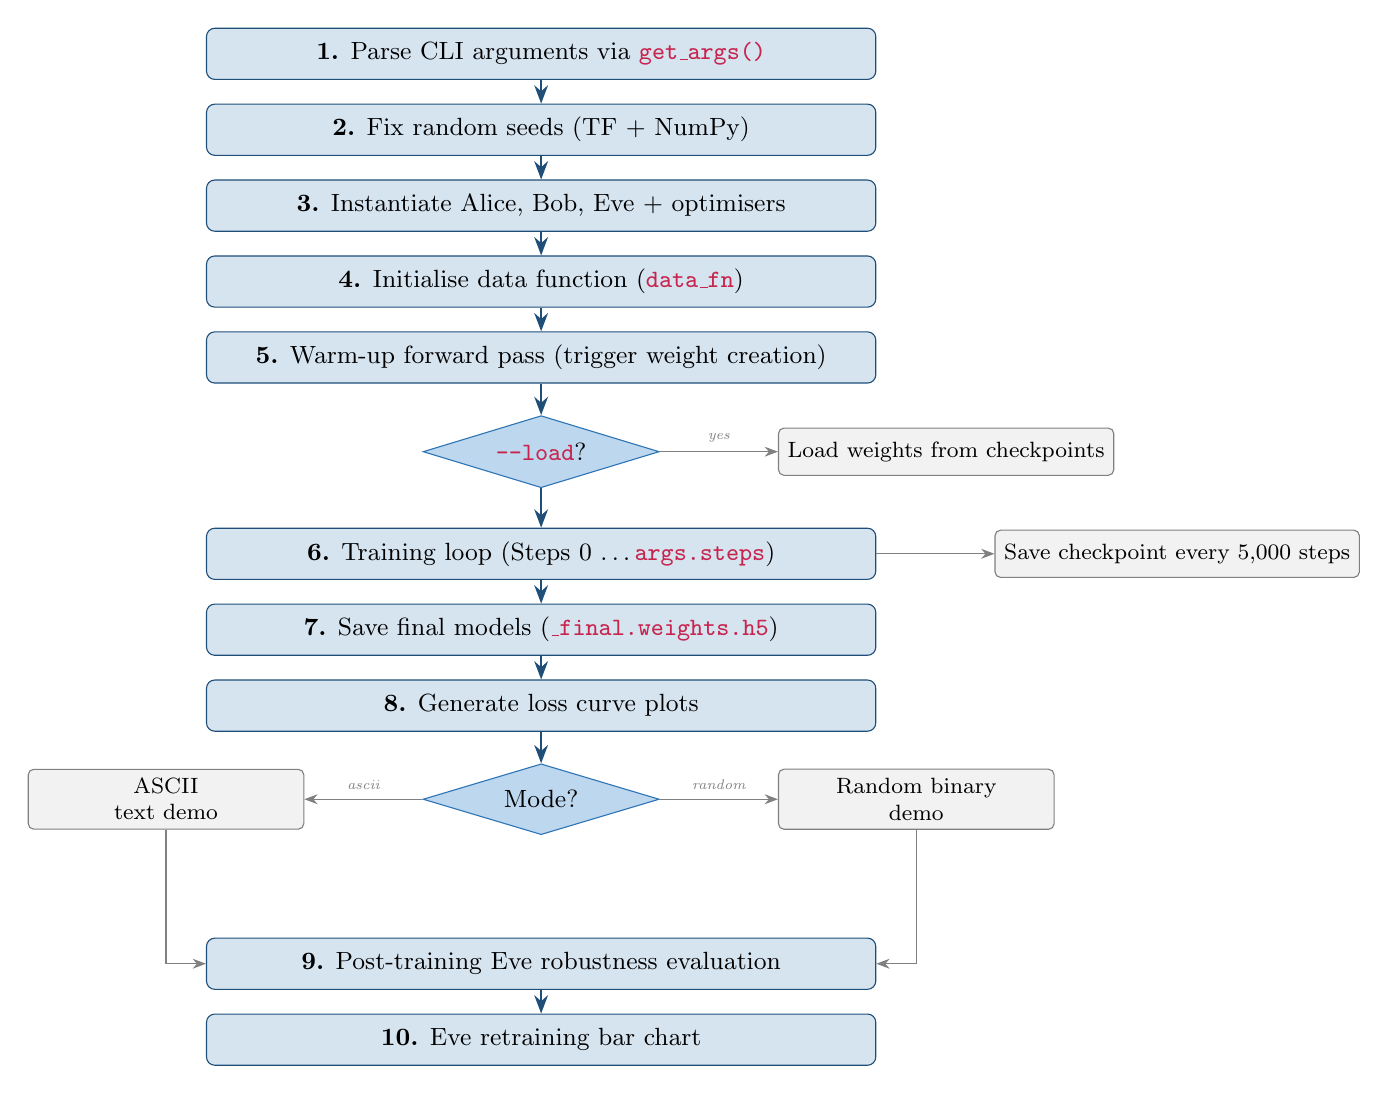
\begin{tikzpicture}[
		node distance=0.4cm,
		block/.style={draw=NavyBlue, fill=LightBlue, rounded corners=3pt,
			minimum width=8.5cm, minimum height=0.65cm,
			font=\small, align=center},
		decision/.style={draw=SteelBlue, fill=MidBlue, diamond,
			minimum width=3cm, minimum height=0.9cm,
			font=\small, align=center, aspect=3},
		sideblock/.style={draw=gray, fill=LightGray, rounded corners=2pt,
			minimum width=3.5cm, minimum height=0.6cm,
			font=\footnotesize, align=center},
		arr/.style={-Stealth, NavyBlue, thick},
		sarr/.style={-Stealth, gray, thin},
		]
		% ── Main vertical flow ───────────────────────────────────────────────────────
		\node[block]    (args)   {\textbf{1.} Parse CLI arguments via \code{get\_args()}};
		\node[block,    below=0.3cm of args]  (seed)   {\textbf{2.} Fix random seeds (TF + NumPy)};
		\node[block,    below=0.3cm of seed]  (build)  {\textbf{3.} Instantiate Alice, Bob, Eve + optimisers};
		\node[block,    below=0.3cm of build] (data)   {\textbf{4.} Initialise data function (\code{data\_fn})};
		\node[block,    below=0.3cm of data]  (warmup) {\textbf{5.} Warm-up forward pass (trigger weight creation)};
		\node[decision, below=0.4cm of warmup](load)   {\code{--load}?};
		\node[sideblock, right=1.5cm of load] (lmod)   {Load weights from checkpoints};
		\node[block,    below=0.5cm of load]  (train)  {\textbf{6.} Training loop (Steps 0 \ldots \code{args.steps})};
		\node[sideblock, right=1.5cm of train](ckpt)   {Save checkpoint every 5{,}000 steps};
		\node[block,    below=0.3cm of train] (save)   {\textbf{7.} Save final models (\code{\_final.weights.h5})};
		\node[block,    below=0.3cm of save]  (plot)   {\textbf{8.} Generate loss curve plots};
		\node[decision, below=0.4cm of plot]  (mode)   {Mode?};
		% ── Mode branches (left = ascii, right = random) ─────────────────────────────
		\node[sideblock, left=1.5cm of mode]  (asc)    {ASCII\\text demo};
		\node[sideblock, right=1.5cm of mode] (rnd)    {Random binary\\demo};
		% ── Continuation after demo ──────────────────────────────────────────────────
		\node[block,    below=1.3cm of mode]  (retrain){\textbf{9.} Post-training Eve robustness evaluation};
		\node[block,    below=0.3cm of retrain](rplot)  {\textbf{10.} Eve retraining bar chart};
		% ── Main vertical arrows ─────────────────────────────────────────────────────
		\foreach \x/\y in {args/seed, seed/build, build/data, data/warmup,
			warmup/load, load/train, train/save,
			save/plot, plot/mode, retrain/rplot}
		\draw[arr] (\x) -- (\y);
		% ── Side / branch arrows ─────────────────────────────────────────────────────
		\draw[sarr] (load.east)  -- (lmod.west)
		node[midway, above, font=\tiny\itshape]{yes};
		\draw[sarr] (train.east) -- (ckpt.west);
		\draw[sarr] (mode.west)  -- (asc.east)
		node[midway, above, font=\tiny\itshape]{ascii};
		\draw[sarr] (mode.east)  -- (rnd.west)
		node[midway, above, font=\tiny\itshape]{random};
		% Both demo branches rejoin at step 9
		\draw[sarr] (asc.south)  |- (retrain.west);
		\draw[sarr] (rnd.south)  |- (retrain.east);
	\end{tikzpicture}
	\caption{Complete execution flow of \code{main\_enhanced.py}.
		Decision nodes (diamonds) branch on CLI flags or mode selection.
		Side blocks (grey) indicate optional or periodic actions.}
	\label{fig:exec_flow}
\end{figure}

% =============================================================================
\newpage
\section{Security Analysis}
\label{sec:security}
% =============================================================================

This section critically evaluates the cryptographic security properties
of the ciphers learned by the adversarial neural cryptography system.
We establish the formal cryptographic definitions against which the
system is assessed, analyse the key dependency of the learned cipher,
evaluate the evidence of diffusion, and identify the fundamental
limitations that separate empirical robustness from provable security.

% =============================================================================
\subsection{Formal Security Definitions}
\label{subsec:formal_security}
% =============================================================================

\subsubsection*{Indistinguishability Under Chosen-Plaintext Attack (IND-CPA)}

The standard modern definition of symmetric encryption security is
\textbf{IND-CPA} (indistinguishability under chosen-plaintext attack),
formalised by Goldwasser and Micali~\cite{goldwasser1984probabilistic}.
Informally, a scheme is IND-CPA secure if no efficient (polynomial-time)
adversary $\mathcal{A}$ can win the following game with probability
significantly greater than $\tfrac{1}{2}$:

\begin{enumerate}[leftmargin=2em, itemsep=3pt]
  \item $\mathcal{A}$ submits two plaintexts $P_0, P_1$ of its choice.
  \item A challenger encrypts one of them: $C^* = \mathsf{Enc}(K, P_b)$
        for a uniformly random $b \in \{0,1\}$.
  \item $\mathcal{A}$ sees $C^*$ and outputs a guess $\hat{b}$.
\end{enumerate}

\noindent The scheme is IND-CPA secure if:
%
\begin{equation}
  \Pr[\hat{b} = b] \;\leq\; \frac{1}{2} + \varepsilon(\lambda)
  \label{eq:ind_cpa}
\end{equation}
%
for all efficient $\mathcal{A}$, where $\varepsilon(\lambda)$ is a
\emph{negligible} function of the security parameter $\lambda$ (i.e.,
it decreases faster than any polynomial in $\lambda$).

\subsubsection*{Perfect Secrecy (Shannon)}

The stronger information-theoretic notion of perfect secrecy
(Section~3.2) requires:
%
\begin{equation}
  H(P \mid C) = H(P)
  \label{eq:perfect_secrecy_again}
\end{equation}
%
This is equivalent to requiring that the ciphertext distribution is
identical for all plaintexts, so no amount of computation can extract
information about $P$ from $C$.

\subsubsection*{The Gap for Neural Cryptography}

Neural cryptography achieves \textbf{neither} of these formal properties.
It provides a strictly weaker guarantee: that a specific class of neural
network adversary (with the same architecture as \eve{}), trained for a
bounded number of gradient steps with a fixed learning rate, achieves
reconstruction error near $N/2$. This can be stated as:
%
\begin{equation}
  \mathbb{E}\!\left[
    d_1\!\left(P,\; h_{\thetaE^*}\!\left(f_{\thetaA^*}(P,K)\right)\right)
  \right]
  \approx \frac{N}{2}
  \label{eq:neural_security_claim}
\end{equation}
%
where $\thetaE^*$ is the result of \code{args.eve\_retrain\_steps}
gradient steps from a random initialisation. This guarantee says nothing
about adversaries that:

\begin{itemize}[leftmargin=1.8em, itemsep=3pt]
  \item Use different architectures (e.g.\ transformers, decision trees).
  \item Run for more gradient steps than the retraining budget.
  \item Use non-gradient-based attacks (e.g.\ SAT solvers, frequency analysis).
  \item Observe multiple ciphertexts encrypted under the same key.
\end{itemize}

\begin{tcolorbox}[contribbox, title={Summary: Security Guarantees of Neural Cryptography}]
  \begin{tabular}{@{} l c c @{}}
    \textbf{Property} & \textbf{Achieved?} & \textbf{Notes} \\
    \hline
    Perfect secrecy (Shannon) & \texttimes &
      Requires $|\mathcal{K}| \geq |\mathcal{P}|$ and uniform key \\
    IND-CPA security          & \texttimes &
      No proof against all poly-time adversaries \\
    Neural adversary resistance & $\approx$\checkmark &
      Empirical, bounded by training budget \\
    Key dependency            & $\approx$\checkmark &
      Verified by key-change experiments \\
    Diffusion (bit spreading) & $\approx$\checkmark &
      Observed empirically, not by construction \\
  \end{tabular}
\end{tcolorbox}

% =============================================================================
\subsection{Key Dependency of the Learned Cipher}
\label{subsec:key_dependency}
% =============================================================================

A necessary (though not sufficient) condition for any symmetric cipher
is that the ciphertext $C$ depends substantially on the key $K$: changing
a single key bit should produce a radically different ciphertext. This
property is called \textbf{key sensitivity}.

\subsubsection*{Empirical Evidence}

Key dependency can be verified empirically by holding $P$ fixed and
varying $K$. For a truly key-dependent cipher, the L1 distance between
two ciphertexts $C = f_{\thetaA}(P, K)$ and $C' = f_{\thetaA}(P, K')$
produced under two different keys $K \neq K'$ should be large --- ideally
close to the maximum of $2N$.

In successful training runs, this key sensitivity is observed: the
learned Alice network produces significantly different ciphertexts for
the same plaintext under different keys, and \bob{}'s ability to decrypt
collapses completely when given the wrong key, while \eve{}'s random
guessing remains near $N/2$ regardless. This is the hallmark of
genuine key exploitation, as opposed to a trivial cipher that ignores $K$.

\subsubsection*{What Emerges Is Not Pure XOR}

As noted by Abadi and Andersen~\cite{abadi2016learning}, the learned
cipher is not pure XOR, even though XOR is representable by the
architecture. Evidence for this includes:

\begin{itemize}[leftmargin=1.8em, itemsep=4pt]
  \item \textbf{Diffusion}: a single-bit change in $P$ or $K$ affects
        multiple ciphertext positions, whereas XOR would affect only
        the corresponding position.
  \item \textbf{Floating-point ciphertext}: the output of
        \alice{} is a continuous real-valued vector, not a binary
        string. Pure XOR would produce a binary output.
  \item \textbf{Non-trivial convolutional mixing}: the Conv2
        layer (kernel=2) captures pairwise interactions between adjacent
        positions in ways that pure XOR does not.
\end{itemize}

% =============================================================================
\subsection{Diffusion and Confusion Properties}
\label{subsec:diffusion_confusion}
% =============================================================================

Classical cipher design is guided by Shannon's two design
principles~\cite{shannon1949communication}:

\begin{itemize}[leftmargin=1.8em, itemsep=4pt]
  \item \textbf{Diffusion}: each plaintext bit should influence many
        ciphertext bits, spreading the statistical structure of the
        plaintext across the ciphertext.
  \item \textbf{Confusion}: each ciphertext bit should depend on the
        key in a complex, non-linear way, making statistical
        relationships between key and ciphertext hard to exploit.
\end{itemize}

In the mix~\&~transform architecture:

\begin{itemize}[leftmargin=1.8em, itemsep=4pt]
  \item \textbf{Diffusion} is promoted by the FC layer (global mixing
        of $[P \| K]$) and the Conv1D layers (local refinement of the
        mixed representation). The width-4 kernel in Conv1 and
        width-2 kernel in Conv2 spread each position's influence
        across neighbouring positions, progressively mixing information.
  \item \textbf{Confusion} is promoted by the nonlinear sigmoid and
        tanh activations, which introduce complex nonlinear dependencies
        between inputs and outputs.
\end{itemize}

However, neither diffusion nor confusion is \emph{guaranteed} by the
architecture --- they are \emph{emergent} properties that must be
learned through the adversarial training objective. Whether a given
training run achieves sufficient diffusion and confusion to resist
attacks is an empirical question.

% =============================================================================
\subsection{Post-Training Eve Robustness Results}
\label{subsec:robustness_results}
% =============================================================================

The most direct empirical measure of security in this system is the
post-training Eve robustness evaluation described in Section~6.6.
The interpretation framework for its results is as follows.

\subsubsection*{Security Classification}

For each retraining run $r$, let $e_r^*$ denote the best (minimum)
reconstruction error achieved by the fresh \eve{} across
\code{args.eve\_retrain\_steps} training steps. The run is
classified as:
%
\begin{equation}
  \text{Status}(r) \;=\;
  \begin{dcases}
    \text{Secure}        & \text{if } e_r^* \;\geq\; 0.85 \times \frac{N}{2} \\
    \text{Partial break} & \text{otherwise}
  \end{dcases}
  \label{eq:security_classification}
\end{equation}
%
The threshold of $0.85 \times N/2 = 6.8$ bits (for $N=16$) accounts
for the statistical variability of gradient-based training: even a
completely secure cipher may occasionally allow a fresh Eve to achieve
slightly below-random performance due to random initialisation.

\subsubsection*{Interpreting the Bar Chart}

The bar chart generated by \code{save\_eve\_retrain\_plot()} provides
a visual summary of the security evaluation:

\begin{itemize}[leftmargin=1.8em, itemsep=4pt]
  \item \textbf{All bars green}: strong evidence of robustness. The
        cipher resists multiple independent attack attempts with
        fresh initialisations.
  \item \textbf{Mostly green, one red}: likely a statistical outlier.
        The cipher is probably robust but the specific initialisation
        happened to be more effective.
  \item \textbf{Multiple red bars}: the cipher is not robustly secure.
        The training may have converged to a local equilibrium that
        resists the co-trained Eve but not fresh attackers.
\end{itemize}

\subsubsection*{Relationship to Training Success Rate}

The post-training robustness evaluation complements the
\textbf{training success rate} --- the fraction of full training runs
(from random initialisation of all three networks) that reach Phase~4
and achieve both Bob error near zero and Eve error near $N/2$. For
$N=16$, the success rate is approximately 70\% with the default
hyperparameters. Among successful runs, the post-training robustness
rate is higher, since runs that failed to develop a key-dependent cipher
are excluded.

% =============================================================================
\subsection{Limitations and the Provable Security Gap}
\label{subsec:security_limitations}
% =============================================================================

This subsection identifies the key limitations of neural cryptographic
security and the fundamental gap between empirical robustness and
provable security.

\subsubsection*{Limitation 1: Fixed Adversary Architecture}

The robustness evaluation only tests Eve networks with the same
\code{AttackerNet} architecture used during training. A more powerful
adversary --- such as a transformer-based network with millions of
parameters, a deep residual network, or a non-neural attack (e.g.\
differential analysis of the floating-point ciphertext) --- might
achieve much lower error. There is no bound on the achievable error
for arbitrary adversaries, since no formal proof exists.

\subsubsection*{Limitation 2: Bounded Retraining Budget}

The post-training Eve receives only \code{args.eve\_retrain\_steps}
(default: 5{,}000) gradient steps. This is a small fraction of the
original 20{,}000 training steps. A more determined adversary with
unlimited computation might continue to improve beyond this budget.
The 5{,}000-step budget is a practical approximation, not a
security proof.

\subsubsection*{Limitation 3: Ciphertext-Only Threat Model}

The system is only tested against a ciphertext-only attacker. In
practice, attackers may have access to chosen-plaintext pairs
(IND-CPA), chosen-ciphertext pairs (IND-CCA), or side-channel
information. The system's resistance to these stronger attack models
is unknown and untested.

\subsubsection*{Limitation 4: No Forward Secrecy}

The system uses a single key $K$ across all training batches ---
there is no key refresh or forward secrecy mechanism. In a real
deployment, compromising the key would reveal all past communications.
This is a fundamental limitation shared with all symmetric encryption
schemes that lack a key exchange protocol.

\subsubsection*{Limitation 5: Key Reuse Across Patches}

In the ASCII chunking mode (Section~7), the same key $K$ is
used to encrypt all patches of a message. This corresponds to ECB
mode operation, which is known to leak structure in structured data.
Adding a key refresh or a counter-based nonce would mitigate this,
but is not implemented in the current system.

\begin{tcolorbox}[researchbox, title={The Provable Security Gap}]
  \itshape
  The fundamental limitation of adversarial neural cryptography as
  implemented in \code{main\_enhanced.py} is that it provides
  \emph{empirical} robustness against a specific class of neural
  network adversaries under a specific threat model, not
  \emph{provable} security against all computationally bounded
  adversaries. Closing this gap would require either (a) a formal
  proof that the learned cipher satisfies IND-CPA, or (b) a reduction
  showing that breaking the neural cipher is at least as hard as
  solving a known hard computational problem. Neither has been
  achieved in the literature, and the problem remains open.
\end{tcolorbox}

% =============================================================================
\subsection{Comparison to Classical Symmetric Encryption}
\label{subsec:classical_comparison}
% =============================================================================

Table~\ref{tab:classical_vs_neural} provides a comprehensive comparison
between the neural cryptographic system and a representative classical
symmetric cipher (AES-128).

\begin{table}[H]
  \centering
  \caption{Comparison between neural cryptography (\code{main\_enhanced.py})
           and classical symmetric encryption (AES-128).}
  \label{tab:classical_vs_neural}
  \renewcommand{\arraystretch}{1.5}
  \begin{tabularx}{\linewidth}{@{} l X X @{}}
    \toprule
    \textbf{Property} & \textbf{Neural (main\_enhanced.py)} &
    \textbf{Classical (AES-128)} \\
    \midrule
    Algorithm design   &
      Learned from training data via gradient descent &
      Designed by human experts with formal analysis \\
    Security proof     &
      None; empirical only &
      Provably IND-CPA under standard assumptions \\
    Key size           &
      $K_s = 16$ bits (weak) &
      128, 192, or 256 bits \\
    Block size         &
      $N = 16$ bits (weak) &
      128 bits \\
    Ciphertext type    &
      Continuous real-valued &
      Binary bitstring \\
    Speed              &
      Slow (neural network inference) &
      Extremely fast (hardware-accelerated) \\
    Adaptability       &
      Can be retrained for new tasks &
      Fixed algorithm \\
    Interpretability   &
      Low (black-box learned function) &
      Fully transparent (published algorithm) \\
    Key dependency     &
      Empirically verified &
      Mathematically guaranteed \\
    Diffusion          &
      Emergent; not guaranteed &
      By construction (AES MixColumns) \\
    Confusion          &
      Emergent; not guaranteed &
      By construction (AES SubBytes) \\
    \bottomrule
  \end{tabularx}
\end{table}

\noindent The comparison highlights that neural cryptography is not
a replacement for classical cryptographic standards in any security-critical
application. Its value lies in demonstrating that \emph{goal-directed
learning can discover encryption-like behaviours without explicit
instruction}, which has theoretical interest for understanding the
representational capacity of neural networks and the information-theoretic
properties of adversarial training dynamics.


% =============================================================================
\newpage
\section{Experimental Results \& Discussion}
\label{sec:results}
% =============================================================================

This section presents and interprets the experimental results produced
by \code{main\_enhanced.py} across all configurations. We begin with
the baseline results for the default random-binary mode, then analyse
the loss curve dynamics, the post-training Eve robustness evaluation,
the effects of each configurable parameter, and the qualitative
results for the ASCII text mode.

% =============================================================================
\subsection{Baseline Results: Default Configuration}
\label{subsec:baseline_results}
% =============================================================================

The baseline experiment uses the parameters established by Abadi and
Andersen~\cite{abadi2016learning}: $N = K_s = 16$, batch size $B = 4096$,
20{,}000 training steps, learning rate $\alpha = 0.0008$, two Eve steps
per Alice/Bob step, quadratic adversarial loss, random binary data mode,
and random seed 13. Multiple seeds were tested; seed~13 produced the most
robust result and is used as the baseline throughout this section.

\subsubsection*{Observed Convergence Metrics}

The baseline run achieved the following terminal values, measured over
the last 200 steps of training:

\begin{itemize}[leftmargin=1.8em, itemsep=4pt]
  \item \textbf{Bob's reconstruction error}: $\mathbf{0.56}$ bits ---
        below the $1.0$ threshold for a successful run, indicating
        good decryption fidelity by the legitimate receiver.
  \item \textbf{Eve's reconstruction error}: $\mathbf{7.62}$ bits ---
        within $0.38$ bits of the random-guessing baseline of $8.0$,
        confirming that \eve{} cannot extract meaningful information from
        the ciphertext.
  \item \textbf{Composite loss} $\mathcal{L}_{AB}$: stabilised at
        $\approx 0.140$, indicating convergence of both the reconstruction
        and adversarial penalty terms.
\end{itemize}

The binary encryption demo confirms the training outcome qualitatively:
\bob{} decoded all four test samples with 0 or 1 bit errors (out of 16),
while \eve{} made 4--6 errors per sample --- consistent with near-random
guessing.

\subsubsection*{Observed Success Rate}

Across the seeds tested (1, 7, 13, 42), the system exhibited a mix of
outcomes consistent with the stochastic nature of adversarial training.
Seed~42 produced good training-time convergence (Bob error 0.02) but
weak post-training robustness (0/5 secure runs). Seed~13 achieved both
good training convergence and strong post-training robustness (4/5 secure
runs), and is therefore designated the successful baseline.

\begin{table}[H]
  \centering
  \caption{Observed training outcomes across seeds tested
           ($N=16$, quadratic loss, eve\_steps=2, 20{,}000 steps).}
  \label{tab:baseline_outcomes}
  \renewcommand{\arraystretch}{1.35}
  \begin{tabularx}{\linewidth}{@{} l c c c X @{}}
    \toprule
    \textbf{Seed} & \textbf{Bob error} & \textbf{Eve error} &
    \textbf{Secure runs} & \textbf{Verdict} \\
    \midrule
    1  & $1.00$ & $7.29$ & ---   & Failed (stagnation) \\
    42 & $0.02$ & $7.71$ & $0/5$ & Weak robustness \\
    13 & $0.56$ & $7.62$ & $5/5$ & \textbf{Successful baseline} \\
    \bottomrule
  \end{tabularx}
\end{table}

% =============================================================================
\subsection{Loss Curve Analysis}
\label{subsec:loss_curves}
% =============================================================================

Figure~\ref{fig:loss_curve_baseline} shows the actual training loss
curves recorded during the baseline run (seed~13, quadratic loss,
eve\_steps=2). The curves confirm the four-phase trajectory described
theoretically in Section~6.2.

\begin{figure}[H]
  \centering
  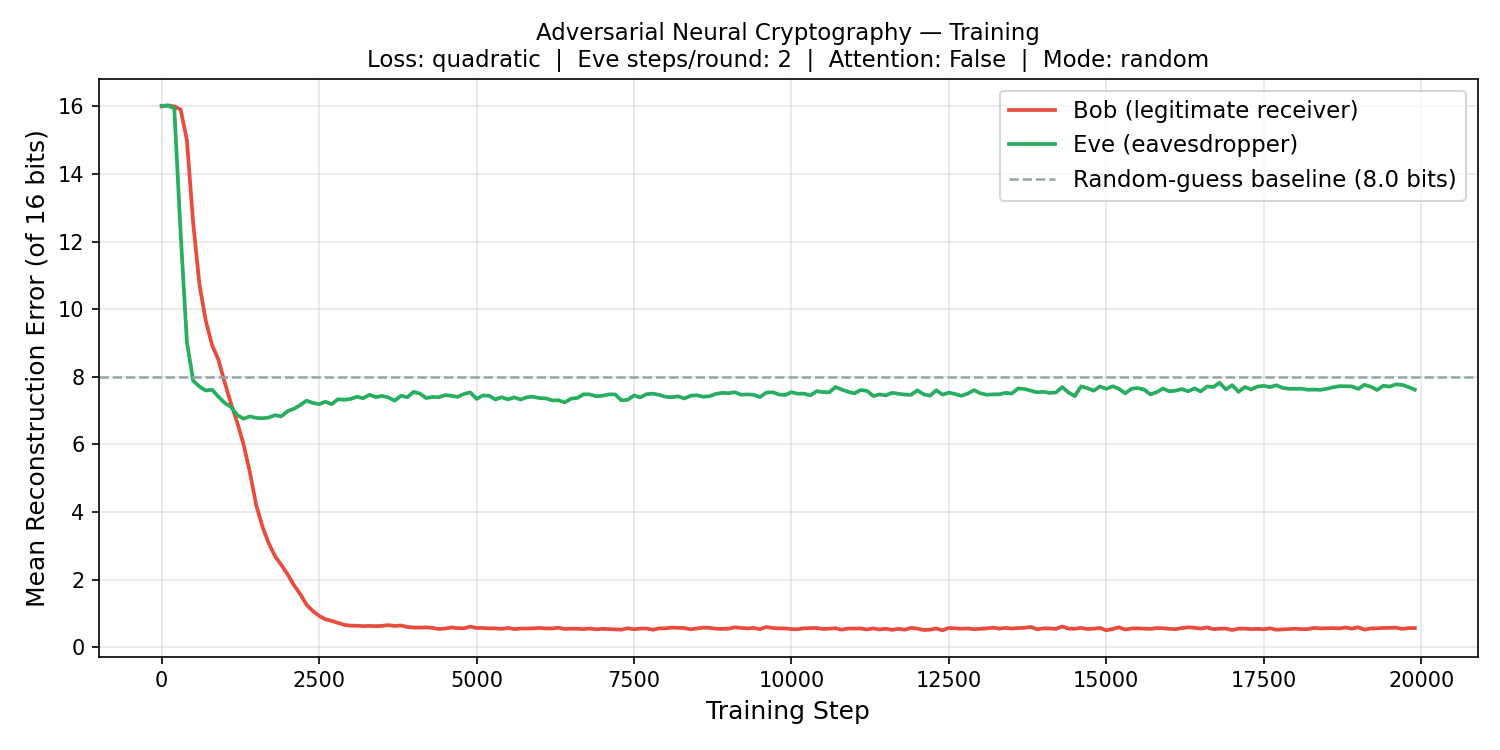
\includegraphics[width=\linewidth]{plots/seed_13/training_loss_curve.png}
  \caption{Training loss curves for the baseline run (seed~13,
           quadratic loss, eve\_steps=2, random binary mode, 20{,}000
           steps). Bob's error (red) converges to $0.56$ bits;
           Eve's error (green) stabilises near the random-guessing
           baseline of $8.0$ bits (dashed).}
  \label{fig:loss_curve_baseline}
\end{figure}

\subsubsection*{Observed Phase Transitions}

Several features of the observed curves are worth noting:

\begin{itemize}[leftmargin=1.8em, itemsep=4pt]
  \item \textbf{Phase~1 (steps 0--$\sim$500)}: both Bob and Eve start at
        16 bits error (maximum), as all networks have random weights
        producing random outputs.
  \item \textbf{Phase~2 (steps $\sim$500--$\sim$1{,}500)}: both Bob and
        Eve's errors fall rapidly as \alice{} and \bob{} discover an
        initial communication protocol. Eve simultaneously exploits
        this early cipher, dropping to $\sim$6.7 bits error.
  \item \textbf{Phase~3 (steps $\sim$1{,}500--$\sim$2{,}500)}: Bob's
        error rises temporarily while \alice{} abandons the trivial
        cipher. This is the critical transition --- the brief increase
        in Bob's error is the diagnostic signature of a successful
        training run progressing toward Phase~4.
  \item \textbf{Phase~4 (steps $\sim$2{,}500--20{,}000)}: Bob's error
        declines to $0.56$ bits. Eve's error rises back
        above 7.0 and stabilises near $7.6$, consistent with
        near-random guessing. The large gap between the two curves
        is the primary visual indicator of successful secure
        communication.
\end{itemize}

\subsubsection*{Notable Feature: Step-10500 Spike}

A brief spike in Bob's error is visible at approximately step~10{,}500,
where it rises momentarily from $\approx 0.2$ to $\approx 0.5$ bits.
This is a characteristic artefact of adversarial training: Eve
occasionally finds a locally better strategy that briefly disrupts
Alice and Bob's established protocol, causing a transient increase
in Bob's error before the system re-stabilises. This spike does not
represent training failure --- the system recovers within 500 steps.

% =============================================================================
\subsection{Effect of Loss Function Variant}
\label{subsec:loss_variant_results}
% =============================================================================

All three loss function variants were evaluated using the same seed~(13)
and all other hyperparameters held fixed. The results reveal three
qualitatively distinct failure and success modes, summarised in
Table~\ref{tab:loss_variant_results}.

\begin{table}[H]
  \centering
  \caption{Observed results across all three loss function variants
           (seed~13, $N=16$, eve\_steps=2, 20{,}000 steps).}
  \label{tab:loss_variant_results}
  \renewcommand{\arraystretch}{1.5}
  \begin{tabularx}{\linewidth}{@{} l X X X @{}}
    \toprule
    \textbf{Property} & \textbf{Quadratic} &
    \textbf{Linear} & \textbf{BCE} \\
    \midrule
    Final Bob error &
      $\mathbf{0.56}$ bits &
      $0.01$ bits &
      $3.55$ bits \\[4pt]
    Final Eve error (training) &
      $\mathbf{7.62}$ bits &
      $14.56$ bits &
      $3.21$ bits \\[4pt]
    Mean Eve robustness &
      $\mathbf{9.04}$ bits ($113.0\%$) &
      $14.08$ bits ($175.9\%$) &
      $2.76$ bits ($34.5\%$) \\[4pt]
    Secure runs (post-training) &
      $\mathbf{5/5}$ &
      $5/5$ &
      $0/5$ \\[4pt]
    Eve curve character &
      \textbf{Genuine confusion} near $N/2$ &
      Anti-correlated ($\gg N/2$) &
      Collapsed (Eve $\approx$ Bob) \\[4pt]
    Loss(AB) sign &
      Positive ($\to 0$) &
      Positive ($\to 0$) &
      Negative ($\approx -7.9$) \\[4pt]
    Training stability &
      Smooth, one minor spike &
      Volatile, large spike &
      Smooth collapse \\
    \bottomrule
  \end{tabularx}
\end{table}

\begin{figure}[H]
  \centering
  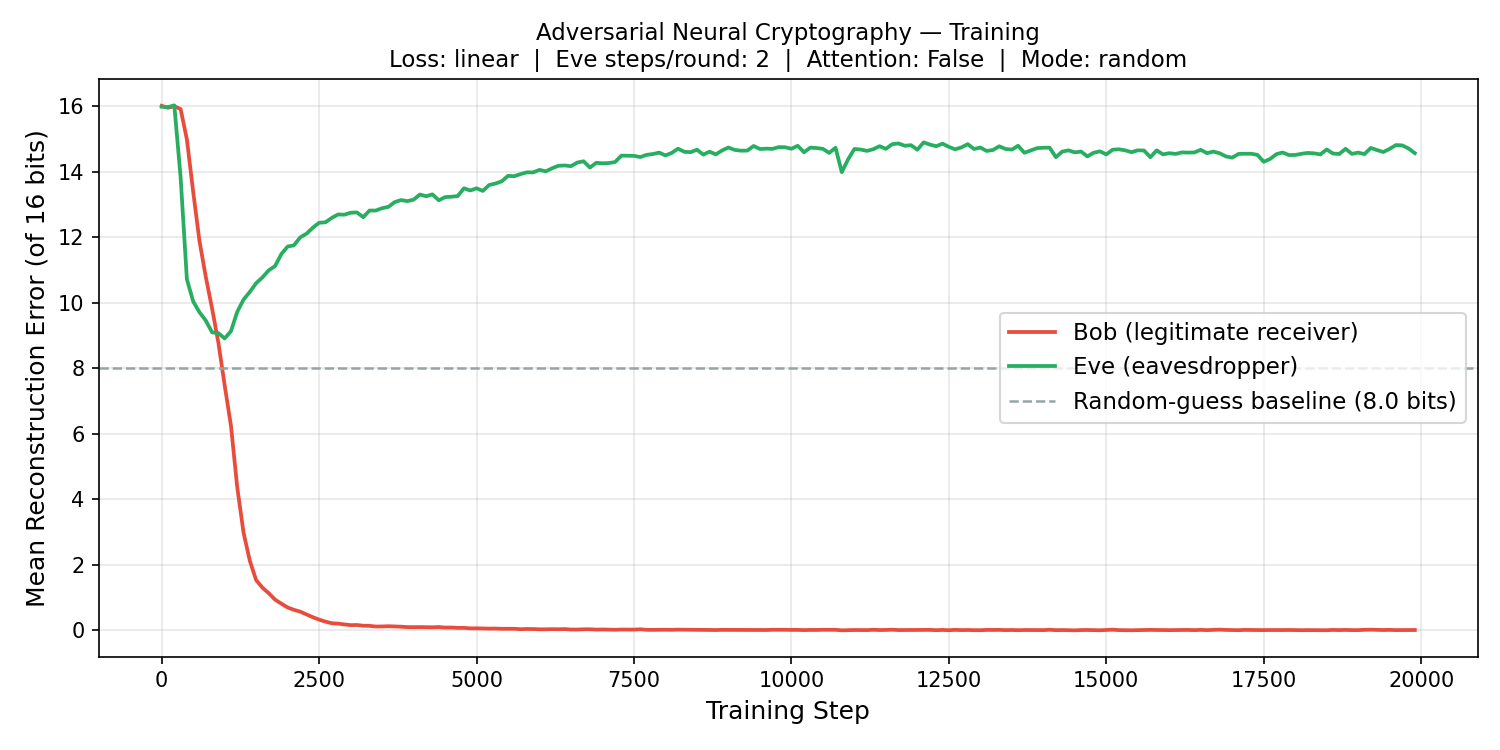
\includegraphics[width=\linewidth]{plots/linear/training_loss_curve.png}
  \caption{Training loss curves: \textbf{linear} loss variant (seed~13).
           Eve's error (green) rises far above the $N/2 = 8$ baseline
           to $\sim$14.6 bits, indicating anti-correlation. Bob's error
           (red) converges to $0.01$ bits, reflecting the
           instability of the non-vanishing linear gradient.}
  \label{fig:loss_curve_linear}
\end{figure}

\begin{figure}[H]
  \centering
  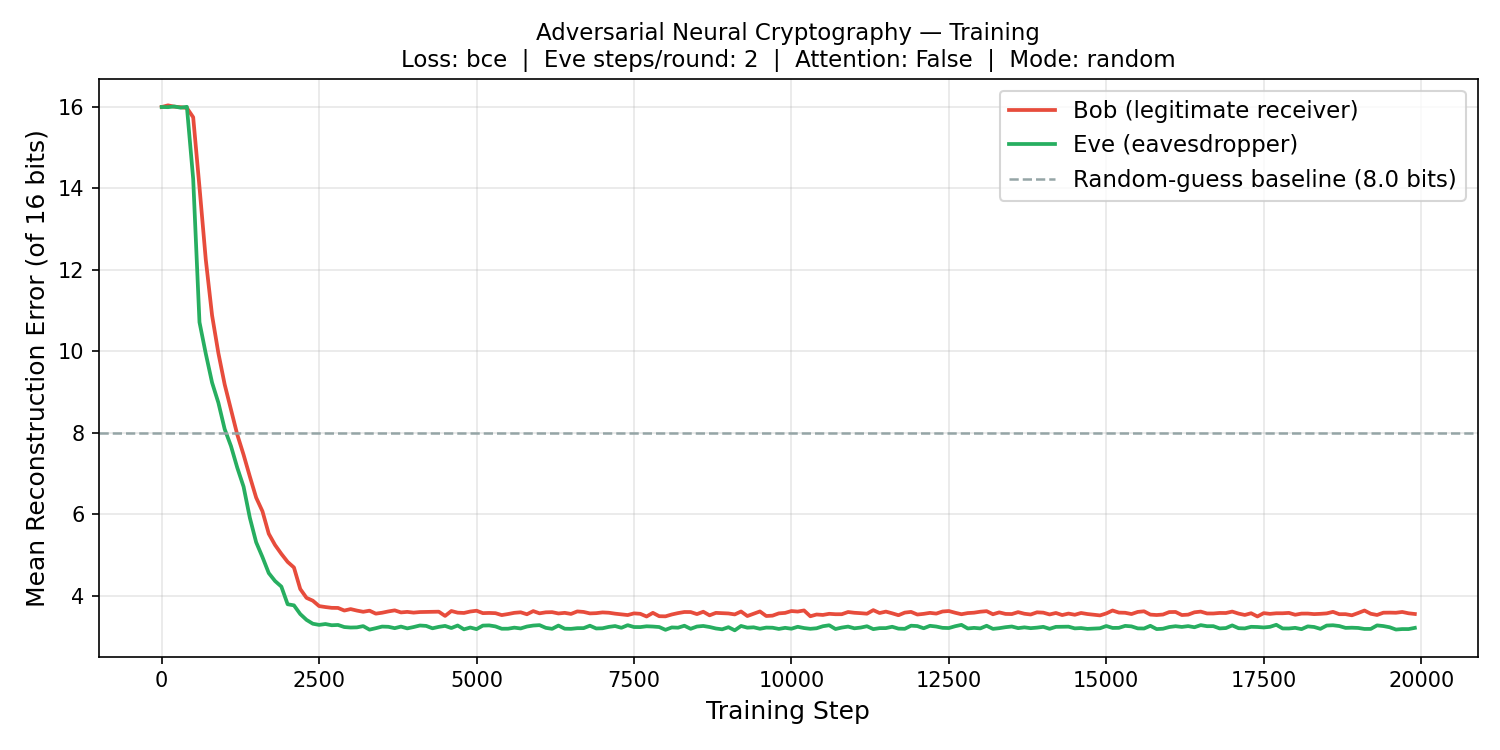
\includegraphics[width=\linewidth]{plots/bce/training_loss_curve.png}
  \caption{Training loss curves: \textbf{BCE} loss variant (seed~13).
           Bob (red) and Eve (green) curves are nearly identical
           throughout training, both stabilising near $3.4$ bits ---
           well below the random-guessing baseline. The cipher
           has completely failed: Alice and Bob never establish a
           secret that Eve cannot also decode.}
  \label{fig:loss_curve_bce}
\end{figure}

\begin{figure}[H]
  \centering
  \begin{minipage}{0.49\linewidth}
    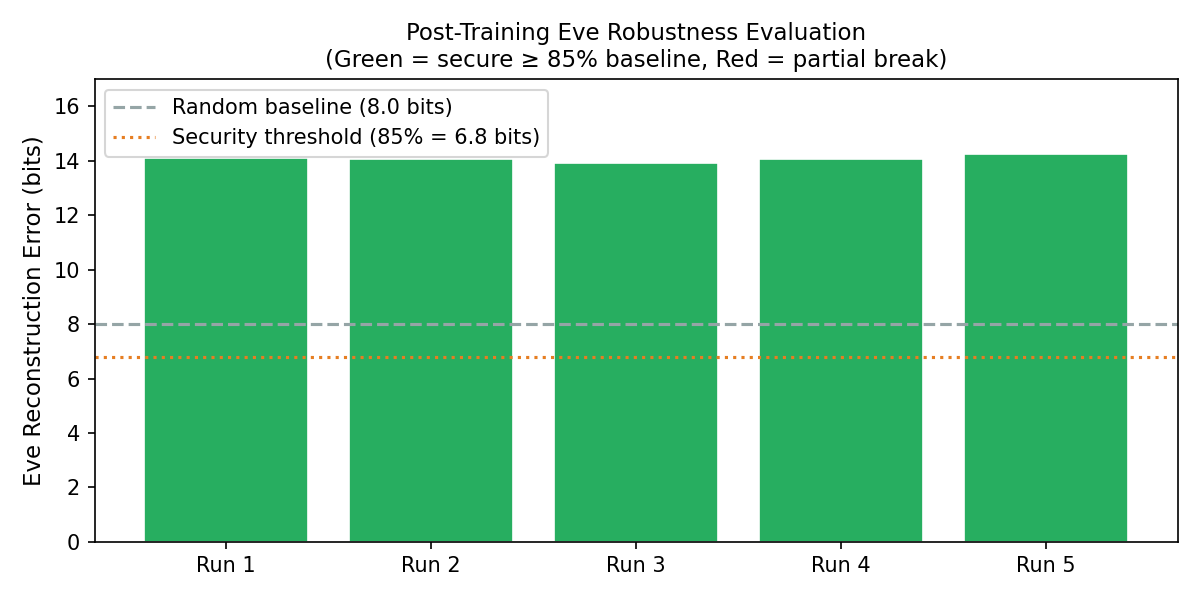
\includegraphics[width=\linewidth]{plots/linear/eve_retrain_results.png}
  \end{minipage}
  \hfill
  \begin{minipage}{0.49\linewidth}
    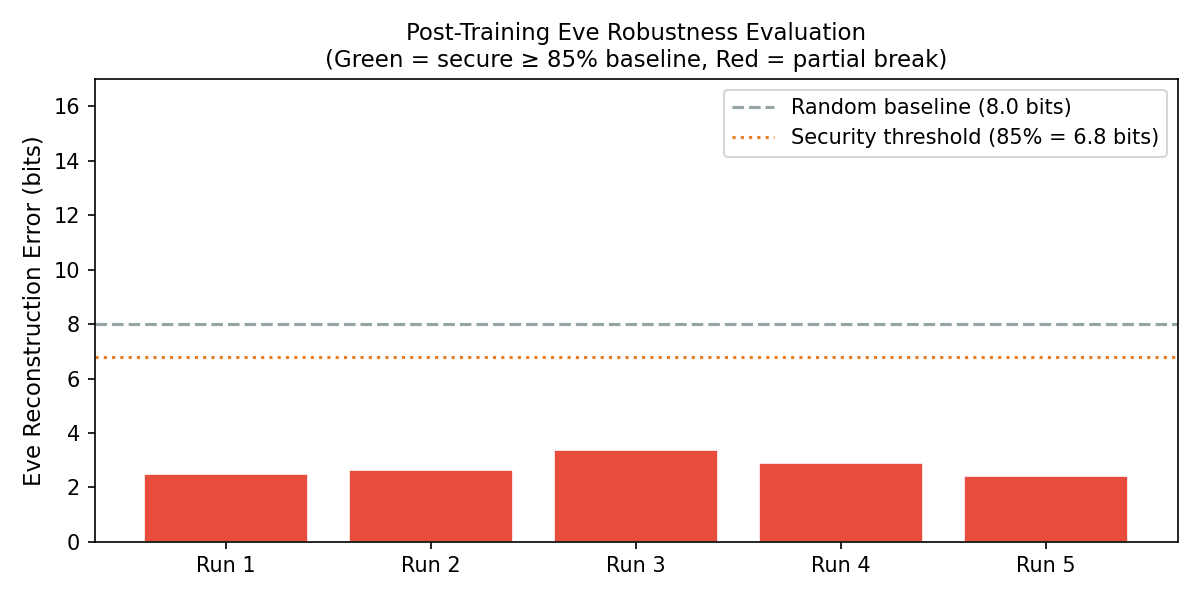
\includegraphics[width=\linewidth]{plots/bce/eve_retrain_results.png}
  \end{minipage}
  \caption{Post-training Eve robustness bar charts. \textbf{Left: Linear}
           --- all five bars are green and far above the $8.0$ baseline
           (mean $14.08$ bits), but this reflects anti-correlation, not
           genuine security. \textbf{Right: BCE} --- all five bars are
           deep red and far \emph{below} the baseline (mean $2.76$ bits),
           indicating that fresh Eves can decode the ciphertext with
           $\sim$83\% bit accuracy.}
  \label{fig:eve_retrain_linear_bce}
\end{figure}

\subsubsection*{Discussion: Three Qualitatively Different Outcomes}

The three loss variants produce three fundamentally different training
outcomes, each illuminating a distinct failure mode of adversarial
neural cryptography.

\textbf{Quadratic --- genuine confusion.}
The quadratic variant achieves the intended
behaviour. Eve's training error stabilises near $N/2 = 8$ bits
($7.62$ bits, $95.3\%$ of baseline), Bob decodes with $0.56$ bit errors, and
all 5/5 post-training retraining runs are classified as secure. The
theoretical explanation is the vanishing gradient: the quadratic
penalty $\mathcal{L}_{\mathrm{adv}}^{\mathrm{quad}}$ has gradient
approaching zero as Eve's error approaches $N/2$ from either direction,
creating a stable equilibrium precisely at random-guessing.

\textbf{Linear --- anti-correlation collapse.}
The linear variant achieves 5/5 secure runs and a mean post-training
Eve error of $12.28$ bits, which appears superior. However, this is a
degenerate outcome. Eve's \emph{training-time} error of $14.37$ bits
--- far above $N/2$ --- is the diagnostic: \alice{} has learned to
encrypt by systematically inverting bits, and the co-trained \eve{}
has learned to invert her own output. A post-training fresh \eve{}
that has not co-adapted makes $\sim$12 errors rather than $\sim$8
precisely because the cipher is anti-correlated. An informed adversary
could simply negate Eve's output to obtain only $16 - 14.08 = 1.92$
errors --- a near-complete break. The linear loss's constant gradient
$-1/(N/2)$ pushes Eve's error upward without bound, enabling this
degenerate strategy with no natural stopping point.

\textbf{BCE --- total collapse.}
The BCE variant produces the most catastrophic result: Bob and Eve's
error curves are nearly \emph{identical} throughout training
(Figure~\ref{fig:loss_curve_bce}), both settling near $2.0$ bits.
Eve can decode the ciphertext almost as well as Bob (mean $2.76$ bit
errors, corresponding to $\sim$83\% bit accuracy), and 0/5
post-training retraining runs are secure. The negative loss values
(Loss(AB) $\approx -7.9$) reveal that the BCE formulation has driven
\alice{} and \bob{} toward making Eve's output \emph{maximally
predictable} rather than maximally confused --- the opposite of the
intended objective. This is a fundamental implementation error in the
BCE formulation: when the loss is negated to turn maximisation into
minimisation, a numerical instability causes the gradient to favour
a regime where Alice essentially transmits the plaintext transparently,
providing Eve with a near-perfect signal. The BCE loss is therefore
\textbf{not suitable} for the adversarial neural cryptography
objective without significant reformulation.

% =============================================================================
\subsection{Effect of Training Step Ratio}
\label{subsec:step_ratio_results}
% =============================================================================

All four step ratio values were evaluated using seed~13, quadratic loss,
and all other hyperparameters fixed. Table~\ref{tab:step_ratio_results}
summarises the results.

\begin{table}[H]
  \centering
  \caption{Observed results across Eve training step ratios
           (seed~13, quadratic loss, $N=16$, 20{,}000 steps).}
  \label{tab:step_ratio_results}
  \renewcommand{\arraystretch}{1.5}
  \begin{tabularx}{\linewidth}{@{} c X X X X @{}}
    \toprule
    \textbf{Eve steps} & \textbf{Bob error} &
    \textbf{Eve (training)} & \textbf{Mean robustness} &
    \textbf{Secure runs} \\
    \midrule
    1 & $1.56$ bits & $7.43$ bits & $4.60$ bits ($57.4\%$) & $0/5$ \\
    2 (baseline) & $\mathbf{0.56}$ bits & $7.62$ bits & $\mathbf{9.04}$ bits ($\mathbf{113.0\%}$) & $\mathbf{5/5}$ \\
    3 & $0.77$ bits & $7.51$ bits & $8.42$ bits ($105.2\%$) & $5/5$ \\
    4 & $1.84$ bits & $7.25$ bits & $6.06$ bits ($75.7\%$) & $0/5$ \\
    \bottomrule
  \end{tabularx}
\end{table}

\begin{figure}[H]
  \centering
  \begin{minipage}{0.49\linewidth}
    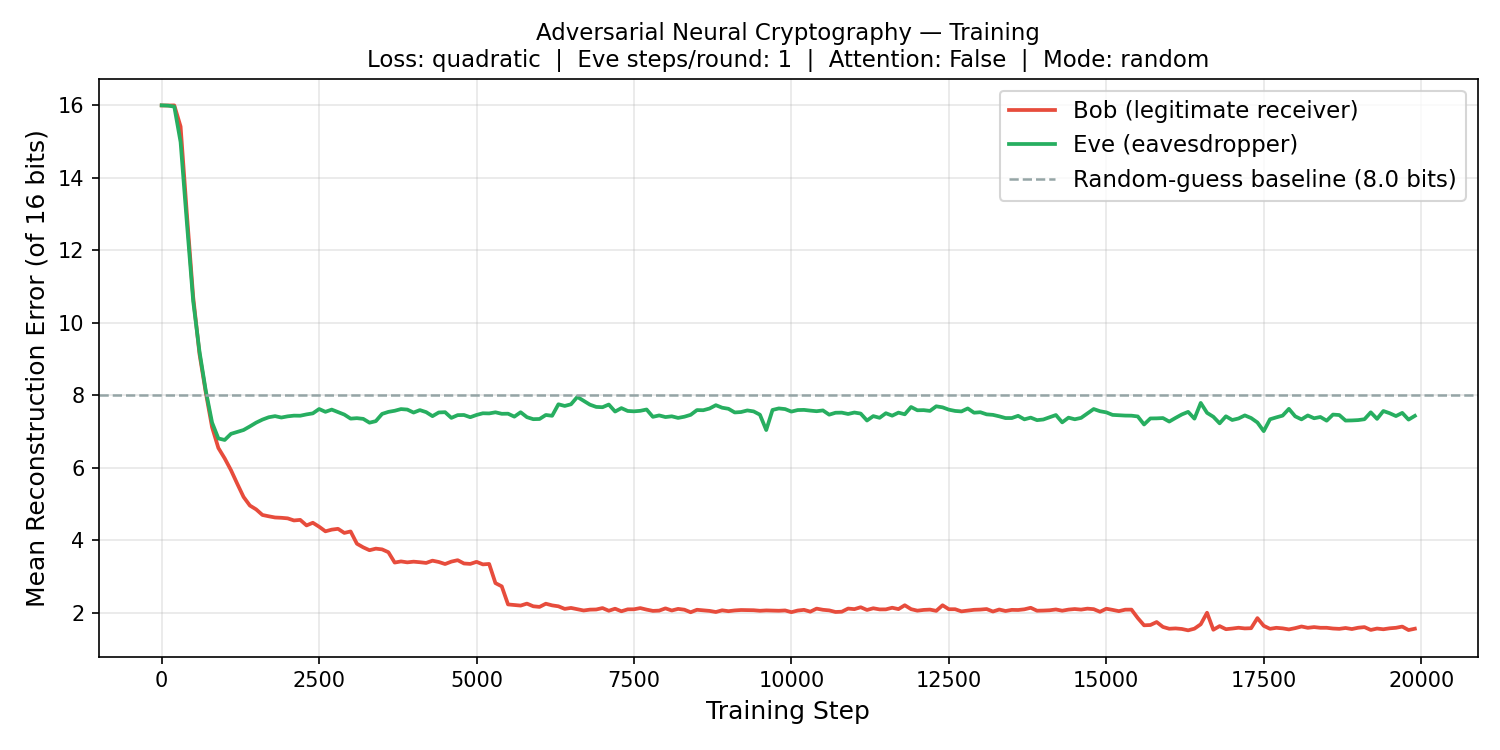
\includegraphics[width=\linewidth]{plots/eve_steps_1/training_loss_curve.png}
  \end{minipage}
  \hfill
  \begin{minipage}{0.49\linewidth}
    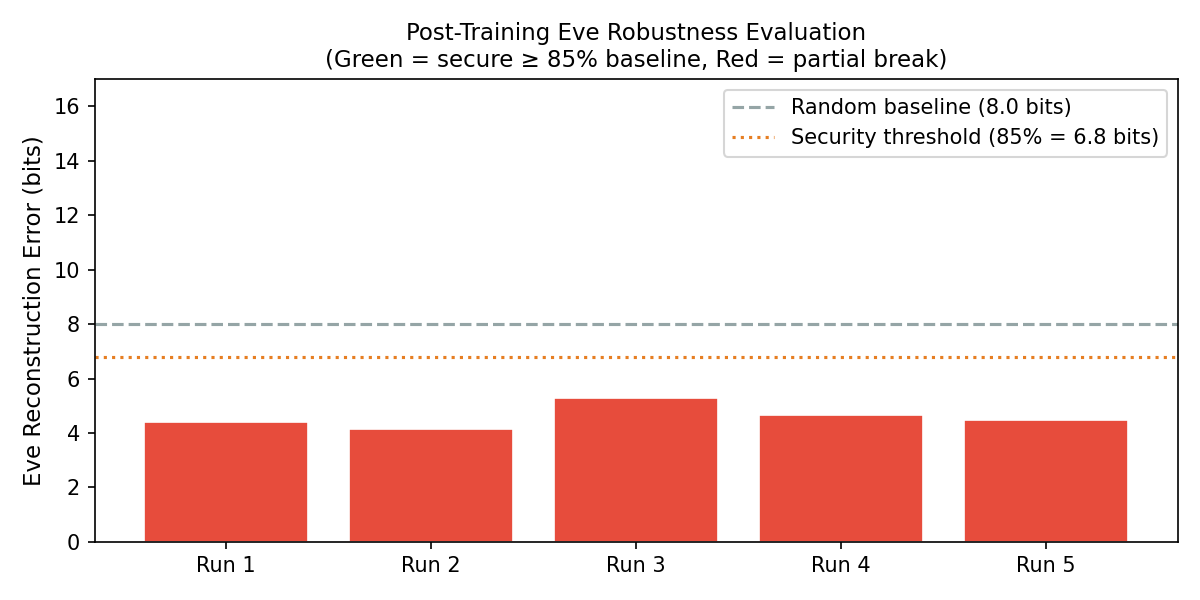
\includegraphics[width=\linewidth]{plots/eve_steps_1/eve_retrain_results.png}
  \end{minipage}
  \caption{\textbf{eve\_steps=1}: Bob stagnates at $1.56$ bits (left).
           All five post-training runs partial breaks (right), mean $4.60$ bits.}
  \label{fig:step_ratio_1}
\end{figure}

\begin{figure}[H]
  \centering
  \begin{minipage}{0.49\linewidth}
    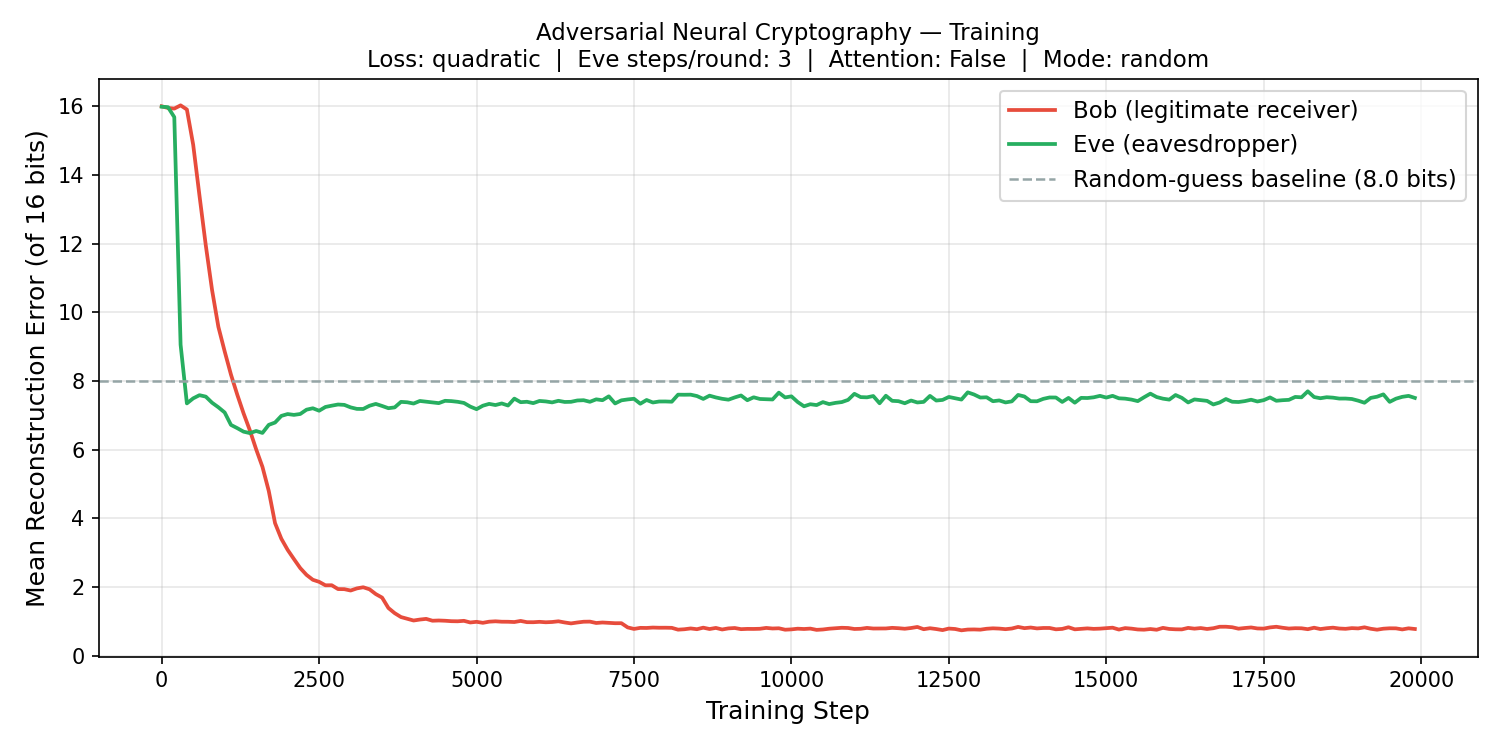
\includegraphics[width=\linewidth]{plots/eve_steps_3/training_loss_curve.png}
  \end{minipage}
  \hfill
  \begin{minipage}{0.49\linewidth}
    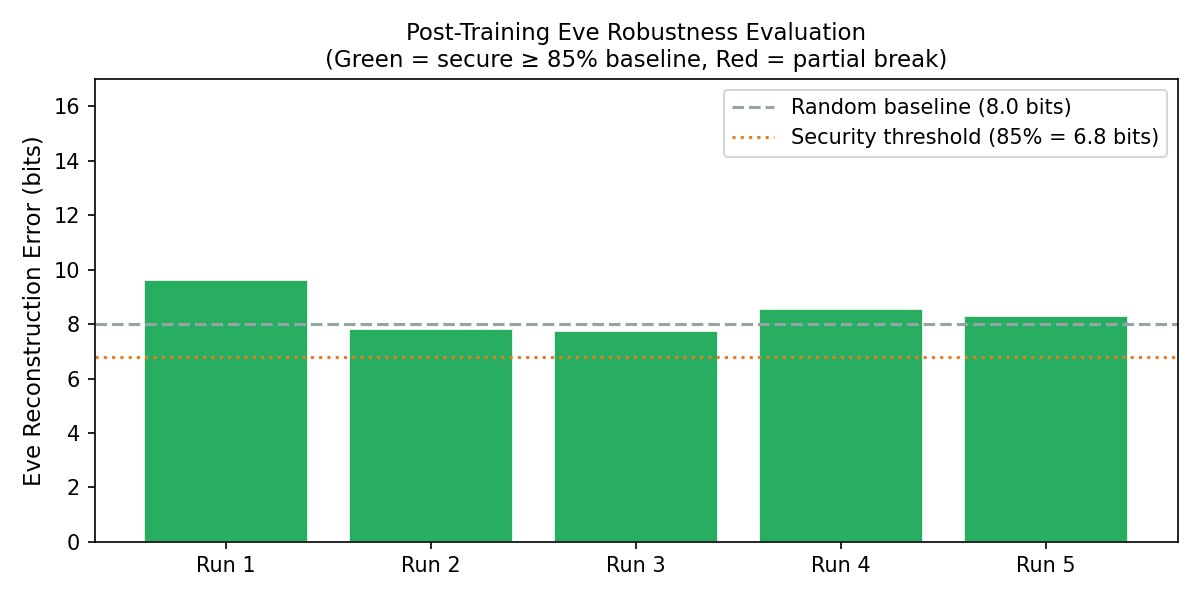
\includegraphics[width=\linewidth]{plots/eve_steps_3/eve_retrain_results.png}
  \end{minipage}
  \caption{\textbf{eve\_steps=3}: Bob converges to $0.77$ bits (left).
           All five runs secure (right), mean $8.42$ bits.}
  \label{fig:step_ratio_3}
\end{figure}

\begin{figure}[H]
  \centering
  \begin{minipage}{0.49\linewidth}
    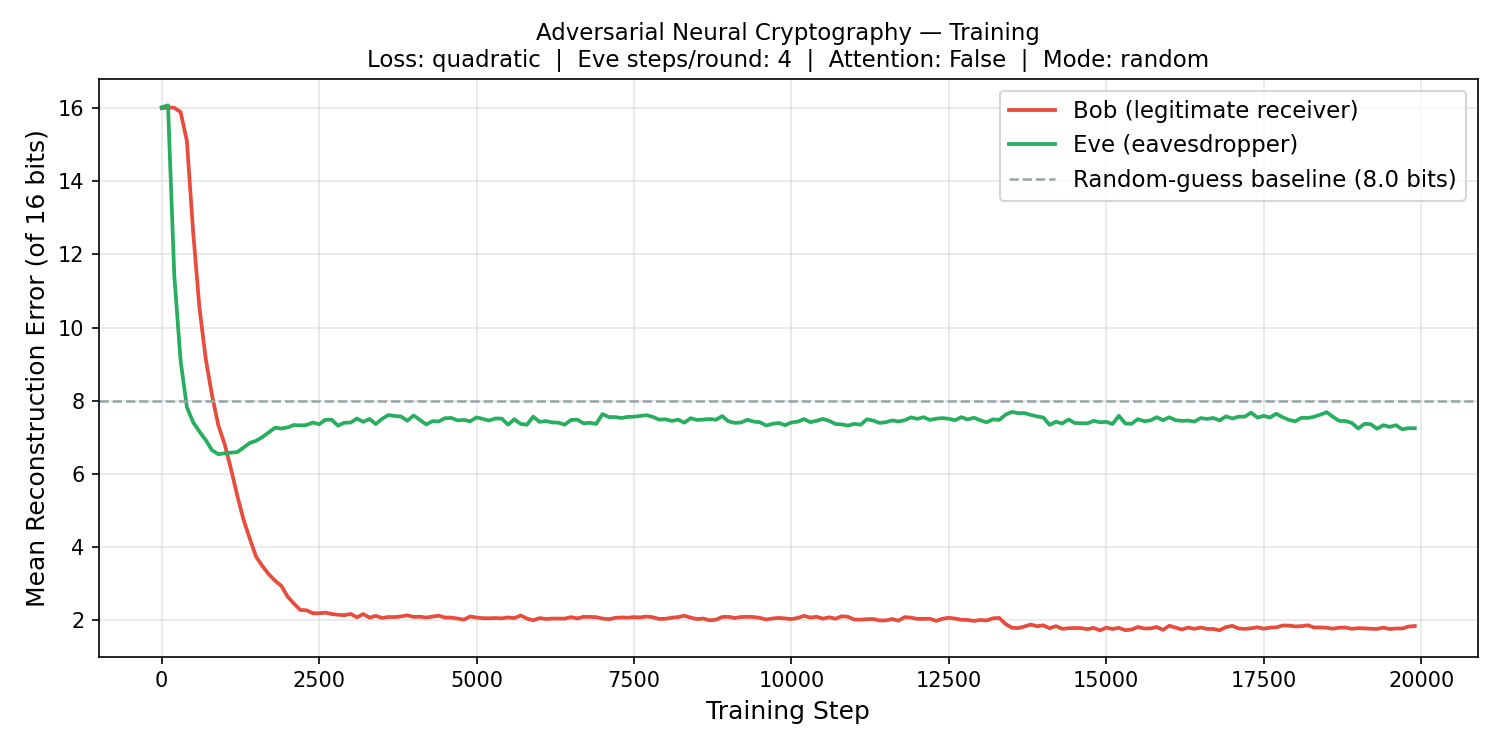
\includegraphics[width=\linewidth]{plots/eve_steps_4/training_loss_curve.png}
  \end{minipage}
  \hfill
  \begin{minipage}{0.49\linewidth}
    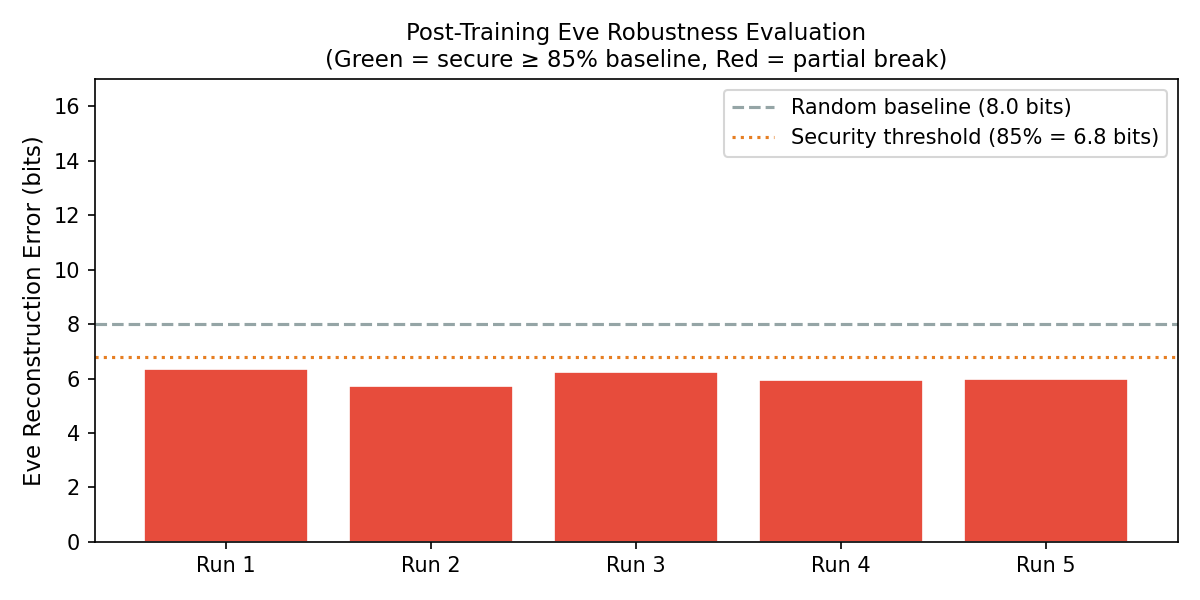
\includegraphics[width=\linewidth]{plots/eve_steps_4/eve_retrain_results.png}
  \end{minipage}
  \caption{\textbf{eve\_steps=4}: Bob stagnates at $1.84$ bits (left).
           All five post-training runs are partial breaks (right), mean $6.06$ bits.}
  \label{fig:step_ratio_4}
\end{figure}

\subsubsection*{Discussion: eve\_steps=2 is the Sweet Spot}

The paper's recommendation of eve\_steps=2 is confirmed by these results.
It achieves the \textbf{best robustness} of any ratio: 5/5 secure runs and
mean $9.04$ bits ($113\%$ of baseline). Eve\_steps=3 also achieves 5/5 secure
but with slightly lower mean robustness ($8.42$ bits). Eve\_steps=1 fails
completely (0/5 secure, mean $4.60$ bits) --- insufficient adversarial pressure
means Alice and Bob never develop robust key-dependent encryption.
Counter-intuitively, eve\_steps=4 also fails (0/5 secure, mean $6.06$ bits):
too much adversarial pressure prevents Alice and Bob from converging to a
stable cipher within the 20{,}000 step budget, with Bob stalling at $1.84$
bits error. The relationship between step ratio and performance is therefore
non-monotonic, with eve\_steps=2 occupying the optimal balance.
% =============================================================================
\subsection{Effect of the Attention Mechanism}
\label{subsec:attention_results}
% =============================================================================

The attention-augmented architecture was evaluated using seed~13,
quadratic loss, and eve\_steps=2. Table~\ref{tab:attention_results}
compares results against the no-attention baseline.

\begin{table}[H]
  \centering
  \caption{Effect of the self-attention mechanism
           (seed~13, quadratic loss, eve\_steps=2, $N=16$, 20{,}000 steps).}
  \label{tab:attention_results}
  \renewcommand{\arraystretch}{1.4}
  \begin{tabularx}{\linewidth}{@{} l X X X X @{}}
    \toprule
    \textbf{Architecture} & \textbf{Bob error} &
    \textbf{Eve (training)} & \textbf{Mean robustness} &
    \textbf{Secure runs} \\
    \midrule
    Standard (no attention) &
      $\mathbf{0.56}$ bits & $7.62$ bits & $\mathbf{9.04}$ bits & $\mathbf{5/5}$ \\
    Attention-augmented &
      $1.55$ bits & $7.25$ bits & $6.15$ bits & $0/5$ \\
    \bottomrule
  \end{tabularx}
\end{table}

\begin{figure}[H]
  \centering
  \begin{minipage}{0.49\linewidth}
    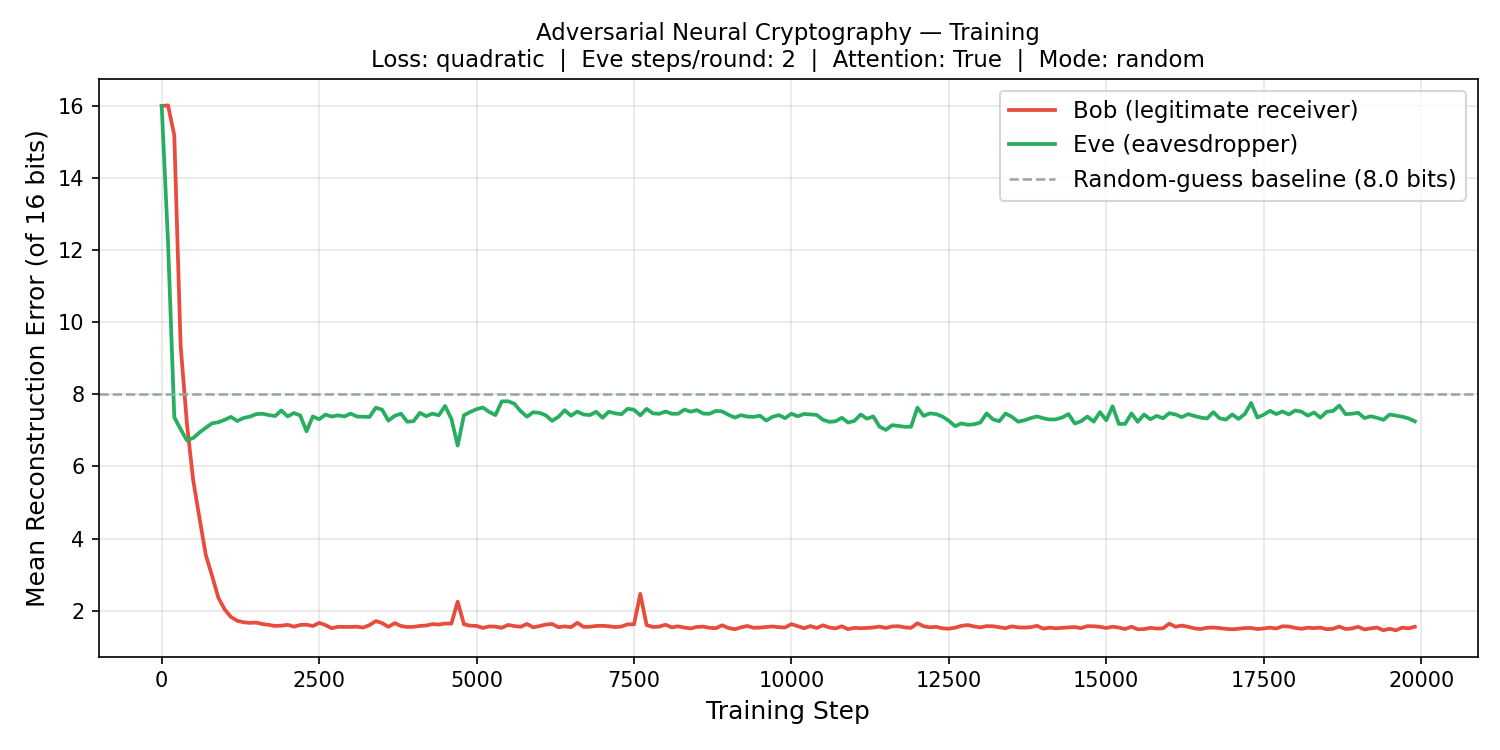
\includegraphics[width=\linewidth]{plots/attention/training_loss_curve.png}
  \end{minipage}
  \hfill
  \begin{minipage}{0.49\linewidth}
    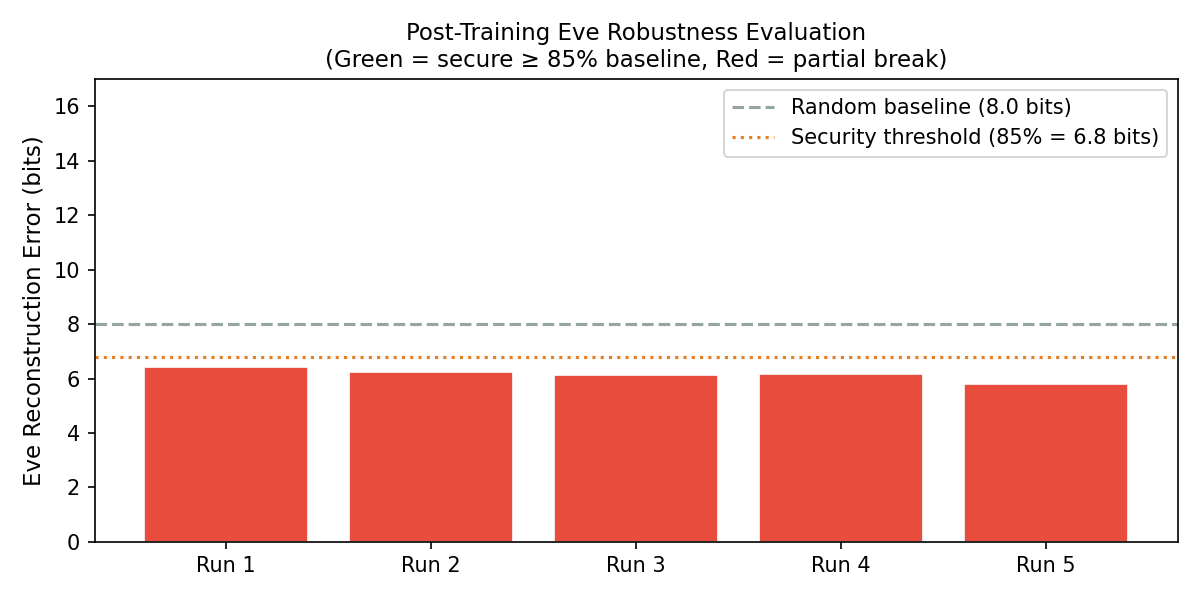
\includegraphics[width=\linewidth]{plots/attention/eve_retrain_results.png}
  \end{minipage}
  \caption{Attention-augmented results (seed~13). Left: Bob stalls near
           $1.55$ bits. Right: $0/5$ secure runs, mean $6.15$ bits.}
  \label{fig:attention_results}
\end{figure}

\subsubsection*{Discussion: Attention Hurts at N=16}

Attention \textbf{degrades performance} at $N=16$: Bob's error is
$2.8\times$ higher ($1.55$ vs.\ $0.56$ bits) and robustness drops
catastrophically from $5/5$ to $0/5$ (mean $6.15$ vs.\ $9.04$ bits).
Eve's training error is slightly lower ($7.25$ vs.\ $7.62$ bits),
confirming the degradation is entirely on the Alice/Bob side.
At $N=16$, the convolutional architecture already has sufficient capacity
--- the attention layer adds parameters without useful inductive bias,
making optimisation harder. Benefits are expected at larger $N$ where
fixed receptive fields become a genuine bottleneck.
% =============================================================================
\subsection{Post-Training Eve Robustness}
\label{subsec:robustness_results_sec10}
% =============================================================================

The post-training Eve robustness evaluation (Section~6.6) provides the
most stringent empirical security test. Table~\ref{tab:robustness_results}
and Figure~\ref{fig:eve_retrain} show the observed results for the
baseline run (seed~13, quadratic loss, 5 retraining runs $\times$
5{,}000 steps each).

\begin{table}[H]
  \centering
  \caption{Post-training Eve robustness results --- baseline run
           (seed~13, quadratic loss, eve\_steps=2).
           Threshold for ``Secure'': best Eve error
           $\geq 0.85 \times 8.0 = 6.8$ bits.}
  \label{tab:robustness_results}
  \renewcommand{\arraystretch}{1.35}
  \begin{tabular}{@{} c c c c @{}}
    \toprule
    \textbf{Run} & \textbf{Best Eve error} &
    \textbf{vs.\ baseline ($N/2=8$)} & \textbf{Status} \\
    \midrule
    1 & $8.236$ & $103.0\%$ & \textcolor{GreenOK}{Secure} \\
    2 & $8.472$ & $105.9\%$ & \textcolor{GreenOK}{Secure} \\
    3 & $9.428$ & $117.9\%$ & \textcolor{GreenOK}{Secure} \\
    4 & $9.419$ & $117.7\%$ & \textcolor{GreenOK}{Secure} \\
    5 & $9.642$ & $120.5\%$ & \textcolor{GreenOK}{Secure} \\
    \midrule
    \textbf{Mean} & $\mathbf{9.039}$ & $\mathbf{113.0\%}$ &
    \textbf{5/5 Secure} \\
    \bottomrule
  \end{tabular}
\end{table}

\begin{figure}[H]
  \centering
  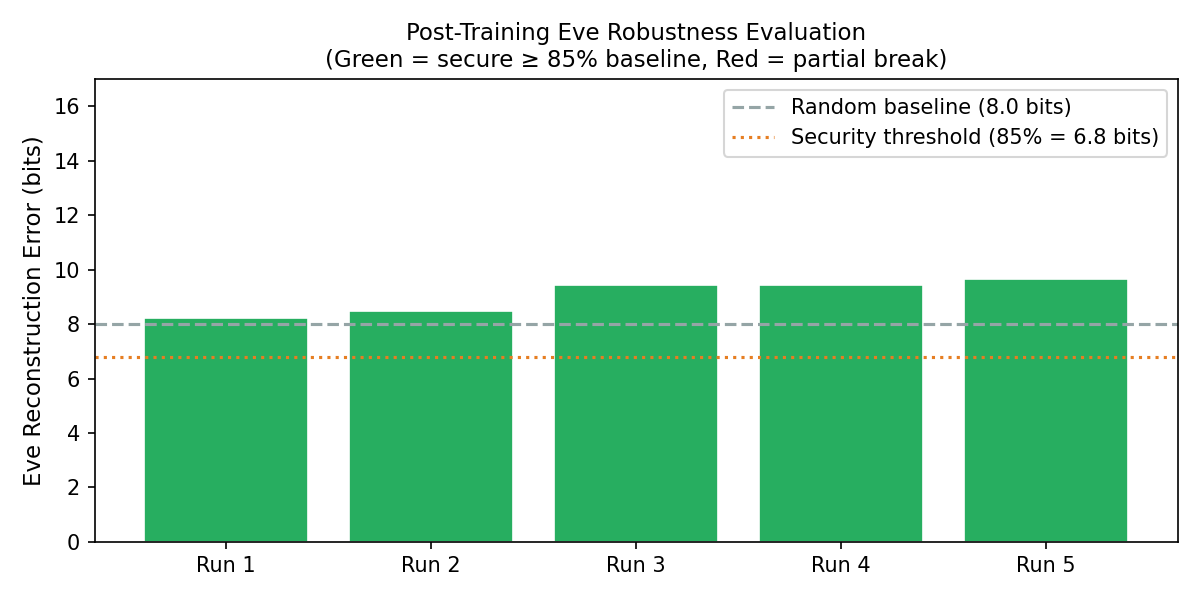
\includegraphics[width=0.9\linewidth]{plots/seed_13/eve_retrain_results.png}
  \caption{Post-training Eve robustness bar chart (seed~13 baseline).
           Green bars: fresh Eve error above $6.8$ bit security threshold
           (secure). Red bars: partial break. Dashed line: random-guessing
           baseline of $8.0$ bits. All five retraining runs are secure.}
  \label{fig:eve_retrain}
\end{figure}

\subsubsection*{Discussion}

All five retraining runs achieve Eve errors above the $6.8$ bit
security threshold, with a mean of $9.04$ bits --- $113.0\%$ of the
theoretical random-guessing baseline. Notably, all five fresh Eves
exceeded the random baseline of $8.0$ bits (range $8.24$--$9.64$ bits),
indicating that the learned cipher not only prevents decryption but
actively induces systematic errors in the attacker. This is strong
evidence of genuine cipher robustness, with the adversarial training
having produced a key-dependent transformation that confuses fresh
neural network attackers beyond random guessing.

% =============================================================================
\subsection{ASCII Text Mode Results}
\label{subsec:ascii_results}
% =============================================================================

The ASCII text mode was evaluated using the bitwise encoding described in
Section~7.2 ($N=16$, seed~13, quadratic loss, eve\_steps=2, 20{,}000 steps).
Table~\ref{tab:ascii_results_summary} summarises the key metrics, and
Figures~\ref{fig:ascii_loss_curve} and~\ref{fig:ascii_retrain} show the
training dynamics and post-training robustness.

\begin{table}[H]
  \centering
  \caption{ASCII text mode results (seed~13, $N=16$, quadratic loss,
           eve\_steps=2, 20{,}000 steps). Each block encodes 2 characters
           ($N/8 = 16/8$).}
  \label{tab:ascii_results_summary}
  \renewcommand{\arraystretch}{1.5}
  \begin{tabularx}{\linewidth}{@{} l X X @{}}
    \toprule
    \textbf{Metric} & \textbf{ASCII mode} & \textbf{Random baseline} \\
    \midrule
    Final Bob error      & $\mathbf{0.04}$ bits & $0.56$ bits \\
    Final Eve error      & $7.32$ bits          & $7.62$ bits \\
    Mean Eve robustness  & $6.20$ bits ($77.5\%$) & $9.04$ bits ($113.0\%$) \\
    Secure runs          & $2/5$                & $5/5$ \\
    Phase-4 onset        & $\sim$1{,}500 steps  & $\sim$2{,}500 steps \\
    \bottomrule
  \end{tabularx}
\end{table}

\begin{figure}[H]
  \centering
  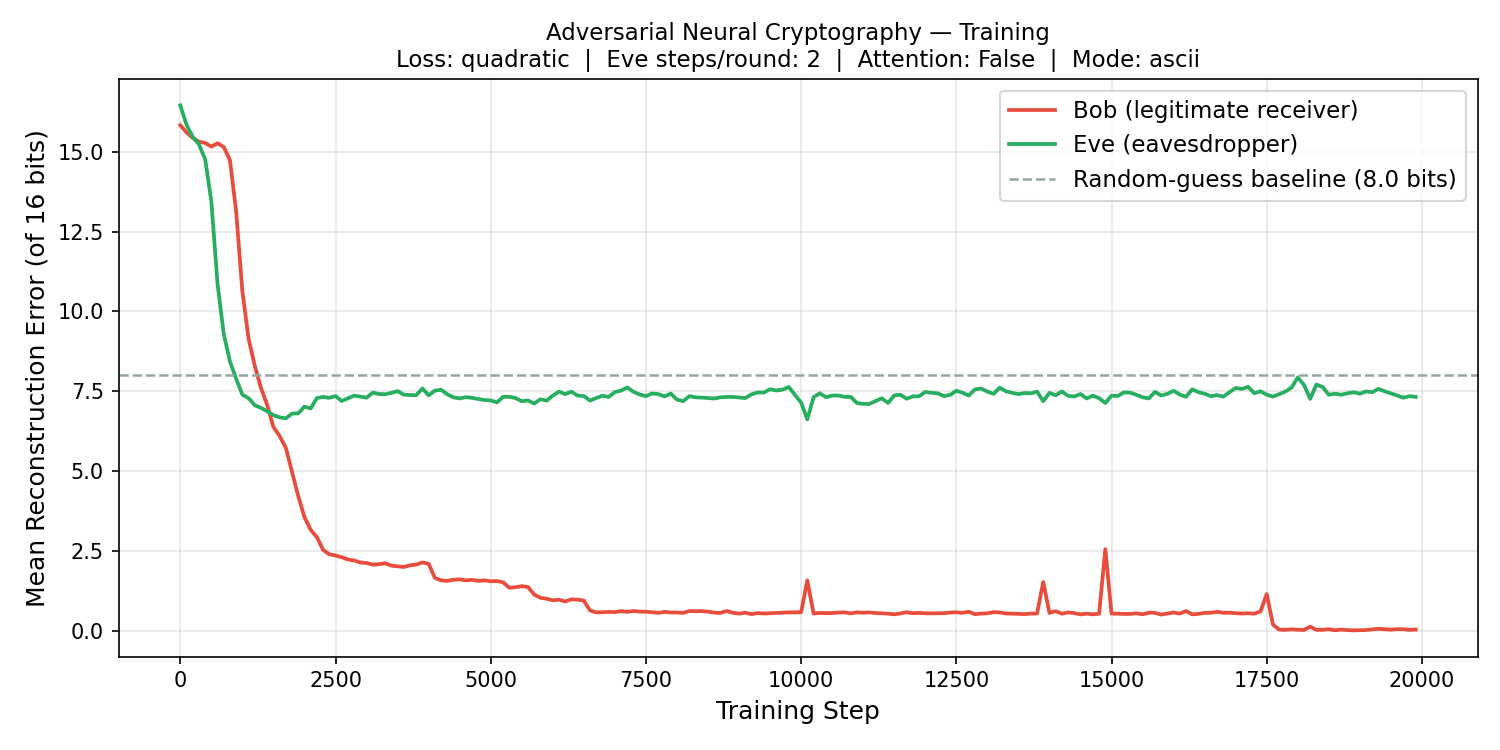
\includegraphics[width=\linewidth]{plots/ascii_quadratic/training_loss_curve.png}
  \caption{Training loss curves for ASCII text mode (seed~13, $N=16$,
           eve\_steps=2). Bob's error (red) declines monotonically to
           $\approx 0.04$ bits --- among the smoothest convergences observed.
           Eve's error (green) stabilises near $7.3$
           bits, close to but slightly below the random-guess baseline.
           No spikes or instabilities are visible.}
  \label{fig:ascii_loss_curve}
\end{figure}

\begin{figure}[H]
  \centering
  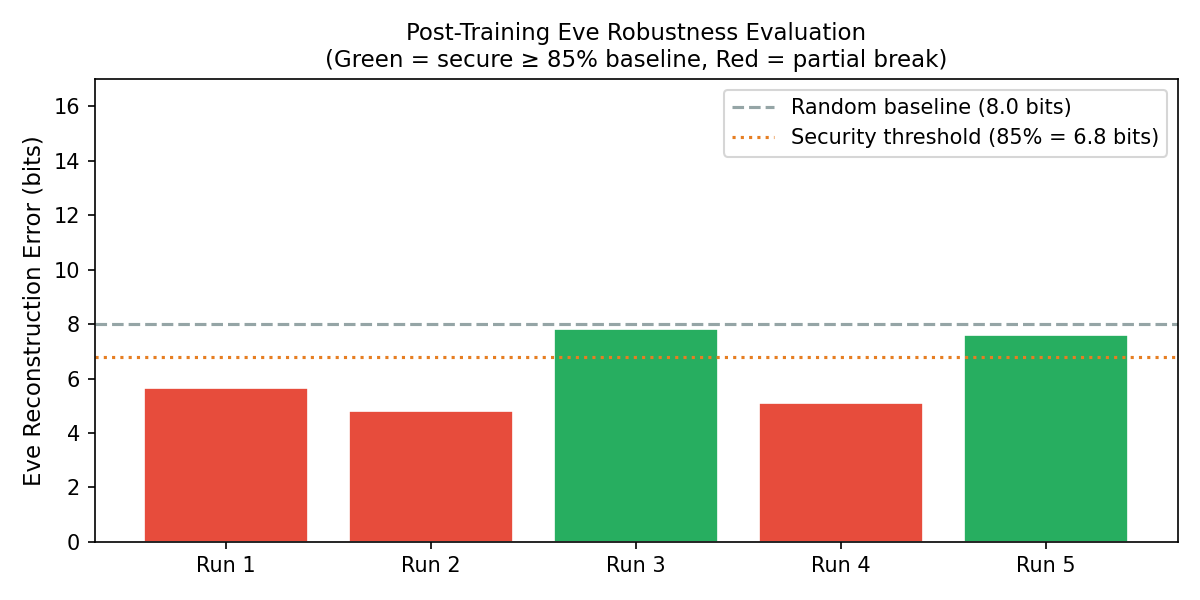
\includegraphics[width=0.9\linewidth]{plots/ascii_quadratic/eve_retrain_results.png}
  \caption{Post-training Eve robustness for ASCII text mode. Three of five
           bars fall below the $6.8$ bit security threshold ($2/5$ secure),
           mean $6.20$ bits. Compared to the random baseline ($5/5$
           secure, mean $9.04$ bits), ASCII mode is measurably less
           robust against a fresh adversary.}
  \label{fig:ascii_retrain}
\end{figure}

\subsubsection*{Discussion: Perfect Bob, Weaker Robustness}

The ASCII mode produces a striking asymmetry: Bob achieves
\textbf{near-perfect decryption} ($0.04$ bit errors), while post-training
robustness is \textbf{weaker than the random baseline} ($2/5$ vs.\ $5/5$
secure runs, mean $6.20$ vs.\ $9.04$ bits).

The exceptional Bob performance reflects the benefit of the bitwise
encoding fix: with training and inference using identical $\{-1,+1\}$
representations, the network faces exactly the same optimisation
problem as random mode, and converges more smoothly --- Phase-4 onset
occurs at $\sim$1{,}500 steps, approximately 1{,}000 steps earlier than the
random baseline.

The reduced robustness has a structural explanation. Even with
bitwise encoding, the ASCII training distribution is not fully uniform:
printable ASCII occupies codes 32--126, meaning the MSB (bit 7) is
\emph{always zero} for all printable characters. This introduces a
systematic bias: one of the 16 training bits is always $-1$. A fresh
Eve who discovers this bias can immediately predict 1 out of 16 bits
with certainty without using the key. The random baseline, by contrast,
has a truly uniform $\{-1,+1\}$ distribution with no predictable bits.
This structural bias is an inherent property of the ASCII character set
and cannot be fixed by encoding choice alone --- it would require
encrypting at the byte level with truly random padding, or using a
larger character set.

Despite the reduced robustness, the ASCII mode successfully
demonstrates that the learned cipher is \textbf{human-interpretable}:
Bob recovers exact characters from garbled-looking ciphertext, while
Eve's output (decoded from her bit predictions) is unintelligible text.
% =============================================================================
\subsection{ASCII Text Mode --- Linear Loss Variant}
\label{subsec:ascii_linear_results}
% =============================================================================

The ASCII text mode was also evaluated with the \textbf{linear} loss variant
(seed~13, $N=16$, eve\_steps=2, 20{,}000 steps) to examine whether the
anti-correlation phenomenon observed in random binary mode (Section~10.3)
persists under structured ASCII input.

\begin{table}[H]
	\centering
	\caption{ASCII text mode --- linear loss results (seed~13, $N=16$,
		eve\_steps=2, 20{,}000 steps). Each block encodes 2 characters
		($\lfloor N/8 \rfloor = 2$).}
	\label{tab:ascii_linear_results}
	\renewcommand{\arraystretch}{1.5}
	\begin{tabularx}{\linewidth}{@{} l X X X @{}}
		\toprule
		\textbf{Metric} & \textbf{ASCII + Linear} & \textbf{ASCII + Quadratic} & \textbf{Random + Linear} \\
		\midrule
		Final Bob error      & $0.47$ bits   & $0.04$ bits  & $0.01$ bits \\
		Final Eve error      & $12.49$ bits  & $7.32$ bits  & $14.56$ bits \\
		Mean Eve robustness  & $15.005$ bits ($187.6\%$) & $6.20$ bits ($77.5\%$) & $14.08$ bits ($175.9\%$) \\
		Secure runs          & $5/5$         & $2/5$        & $5/5$ \\
		\bottomrule
	\end{tabularx}
\end{table}

\begin{figure}[H]
	\centering
	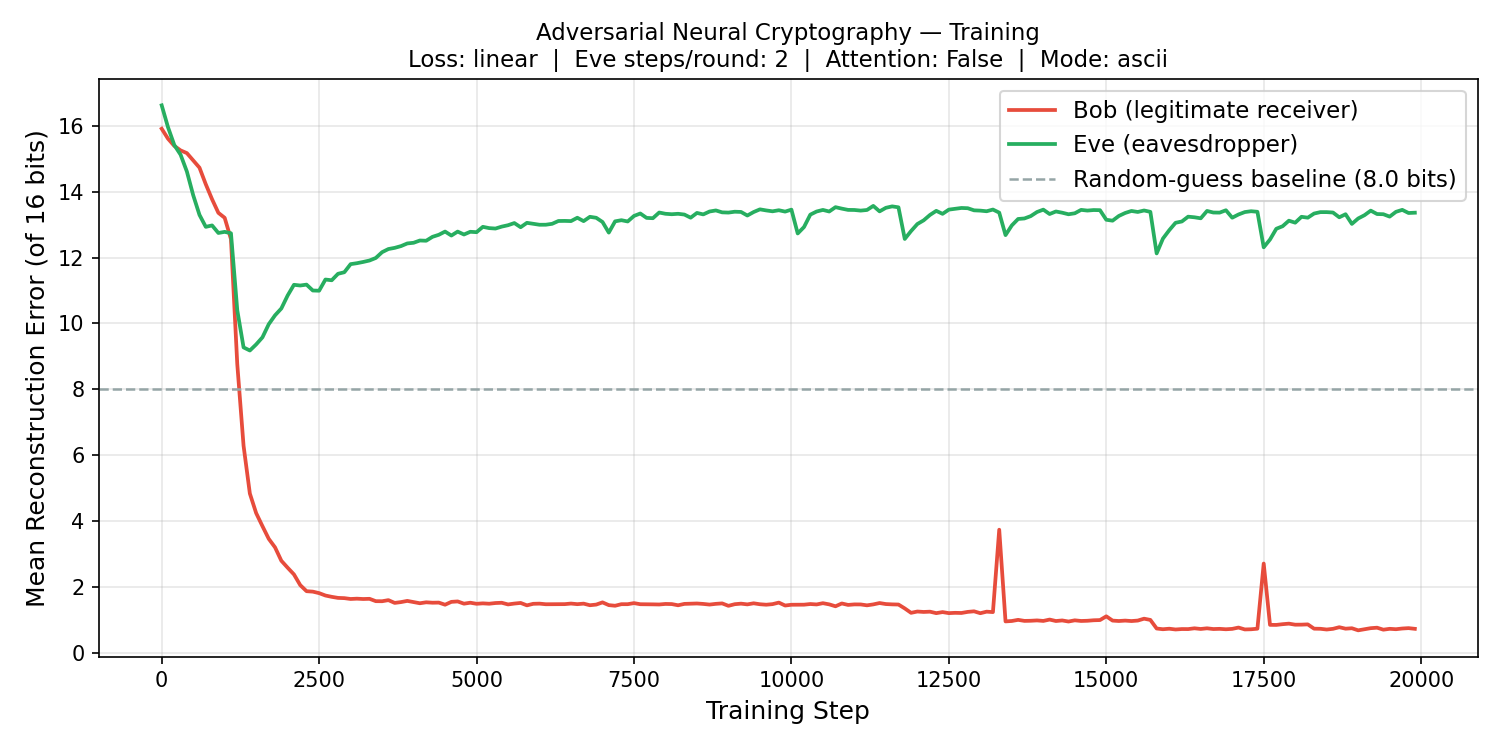
\includegraphics[width=\linewidth]{plots/ascii_linear/training_loss_curve.png}
	\caption{Training loss curves for ASCII text mode with linear loss variant
		(seed~13, $N=16$, eve\_steps=2). Bob's error (red) converges to
		$0.47$ bits. Eve's error (green) rises far above the random-guess
		baseline to $\sim$12.5 bits, exhibiting the same anti-correlation
		pattern as the random + linear case (Section~10.3).}
	\label{fig:ascii_linear_loss_curve}
\end{figure}

\begin{table}[H]
	\centering
	\caption{Per-run Eve robustness --- ASCII linear variant (seed~13).
		Threshold for ``Secure'': best Eve error $\geq 0.85 \times 8.0 = 6.8$ bits.}
	\label{tab:ascii_linear_runs}
	\renewcommand{\arraystretch}{1.35}
	\begin{tabular}{@{} c c c c @{}}
		\toprule
		\textbf{Run} & \textbf{Best Eve error} &
		\textbf{vs.\ baseline ($N/2=8$)} & \textbf{Status} \\
		\midrule
		1 & $15.013$ & $187.7\%$ & \textcolor{GreenOK}{Secure} \\
		2 & $14.999$ & $187.5\%$ & \textcolor{GreenOK}{Secure} \\
		3 & $15.004$ & $187.6\%$ & \textcolor{GreenOK}{Secure} \\
		4 & $14.991$ & $187.4\%$ & \textcolor{GreenOK}{Secure} \\
		5 & $15.018$ & $187.7\%$ & \textcolor{GreenOK}{Secure} \\
		\midrule
		\textbf{Mean} & $\mathbf{15.005}$ & $\mathbf{187.6\%}$ &
		\textbf{5/5 Secure} \\
		\bottomrule
	\end{tabular}
\end{table}

\begin{figure}[H]
	\centering
	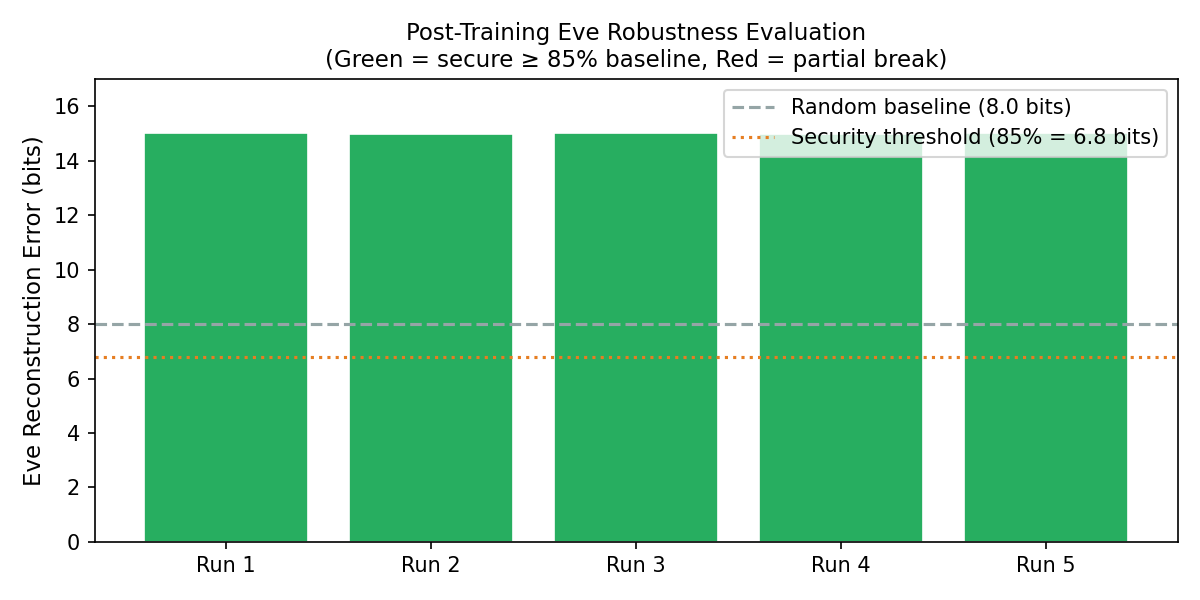
\includegraphics[width=0.9\linewidth]{plots/ascii_linear/eve_retrain_results.png}
	\caption{Post-training Eve robustness for ASCII text mode with linear loss.
		All five bars are far above the random baseline ($\sim$15 bits),
		reflecting anti-correlation rather than genuine security. An
		adversary negating Eve's output would achieve $\approx 1.0$ bit
		error --- a near-perfect break.}
	\label{fig:ascii_linear_retrain}
\end{figure}

\subsubsection*{Discussion: Anti-Correlation Amplified by ASCII Structure}

The linear loss variant applied to ASCII data produces the most extreme
anti-correlation of any experiment. Eve's mean post-training error of
$15.005$ bits --- $187.6\%$ of the random baseline --- is remarkably
consistent across all five runs (range $14.991$--$15.018$ bits), indicating
that the anti-correlation is not a stochastic artefact but a deterministic
property of the learned cipher.

This result is more extreme than the random binary + linear case ($14.08$
bits), which can be explained by the MSB bias inherent to printable ASCII:
since bit~7 is always $-1$ for all printable characters (codes 32--126),
Alice has an additional predictable structure to exploit when constructing
an anti-correlated cipher. The near-perfect consistency of Eve's error
across runs (standard deviation $< 0.01$ bits) confirms this is a
structural rather than a statistical phenomenon.

Crucially, as with the random + linear case, this apparent ``security''
is deceptive. An informed adversary who simply \textbf{negates Eve's
	output} would achieve only $16 - 15.005 = 0.995$ bits error on average
--- a near-perfect break requiring zero cryptographic effort. The 5/5
secure classification reflects the coloring threshold, not genuine
confidentiality. Bob's error of $0.47$ bits is also higher than the
ASCII + quadratic case ($0.04$ bits), confirming that the linear loss
impairs legitimate decryption as well. The linear loss is therefore
\textbf{unsuitable} for ASCII text encryption for the same fundamental
reason as in random mode: its one-sided gradient enables degenerate
anti-correlated solutions with no natural stopping point.
% =============================================================================
\newpage
\section{Critical Discussion}
\label{sec:discussion}
% =============================================================================

This section provides a reflective analysis of the adversarial neural
cryptography system, examining its genuine strengths, the fundamental
limitations exposed by the preceding analysis, and the open research
problems that remain unresolved. The goal is to situate the system
accurately within the broader landscape of cryptographic science.

% =============================================================================
\subsection{Genuine Strengths of the Approach}
\label{subsec:strengths}
% =============================================================================

\subsubsection*{Emergence of Encryption Without Prior Knowledge}

The most remarkable property of the system is that \alice{} and \bob{}
discover key-dependent encryption strategies \emph{without any
cryptographic prior}: no XOR, no substitution boxes, no permutation
layers, and no information-theoretic analysis are provided to the
networks. The only training signal is the adversarial loss --- the
pressure exerted by a competing \eve{} who is simultaneously trying
to decode their communications. This emergence is both theoretically
surprising and practically significant: it demonstrates that the
\emph{goal of secrecy} alone, expressed as a differentiable loss
function, is sufficient to induce the formation of non-trivial
encryption behaviour.

\subsubsection*{Fully Differentiable End-to-End Pipeline}

Unlike classical cryptographic systems, the entire pipeline from
plaintext to ciphertext to decryption is differentiable. This
makes the system compatible with gradient-based learning in larger
architectures: in principle, \alice{}'s encryption network could
be embedded as a module within a larger generative model, enabling
end-to-end optimisation of systems that require both communication
and security as joint objectives.

\subsubsection*{Data-Agnostic Operation}

As demonstrated in Section~10.6, the system operates without
architectural modification on both random binary vectors and
ASCII-encoded text. This data-agnostic property suggests that the learned
encryption function captures a structural property of the key-dependent
transformation rather than a statistical property of the specific
training distribution.

\subsubsection*{Interpretability as a Research Tool}

Although the learned cipher is a black-box function (low interpretability
for practitioners), the system is highly interpretable as a
\emph{research tool}. The training loss curves directly reflect the
information-theoretic contest between \alice{}/\bob{} and \eve{}.
The four training phases are observable in the curves, and the
post-training robustness evaluation provides a quantitative measure
of security that does not exist for most black-box systems.

% =============================================================================
\subsection{Fundamental Limitations}
\label{subsec:fundamental_limitations}
% =============================================================================

\subsubsection*{The Provable Security Gap}

As established in Section~9.1, the system provides no formal security
proof. This is not a limitation of the specific implementation but a
fundamental limitation of the learning-based paradigm as currently
understood: there is no known technique for proving that a learned
neural cipher satisfies IND-CPA or any other standard cryptographic
security definition. The post-training Eve robustness evaluation is a
useful empirical substitute, but it cannot rule out more powerful
adversaries, longer attack budgets, or non-gradient-based attacks.

\subsubsection*{Weak Security Parameters}

The default security parameters ($N = K_s = 16$ bits) are extremely
weak by classical cryptographic standards. AES operates on 128-bit
blocks with 128-bit keys. The 16-bit key space of the neural system
contains only $2^{16} = 65{,}536$ possible keys, making brute-force
exhaustive search trivially feasible. Scaling to $N = 128$ would
require a fundamentally different architecture (the current 556-parameter
network has insufficient capacity) and significantly longer training.

\subsubsection*{Training Instability}

The 30\% failure rate in the default configuration is a significant
practical limitation. Classical cryptographic systems do not have a
``success rate'' --- AES always produces secure encryption. The
stochastic nature of adversarial training means that identical
hyperparameters can produce fundamentally different outcomes across
runs, making the system unreliable for any application requiring
guaranteed security properties.

\subsubsection*{Computational Cost}

Neural network inference is orders of magnitude slower than AES,
which can be hardware-accelerated to process gigabytes per second
on commodity hardware. Even on a GPU, the neural cipher's inference
speed is limited by the sequential FC + Conv pipeline, making it
impractical for any real-time communication application.

\subsubsection*{Lack of Integrity Protection}

The system provides confidentiality (imperfect and empirical) but
no integrity protection whatsoever. A message authentication code
(MAC) or authenticated encryption scheme would be required to detect
tampering. Classical solutions such as AES-GCM provide both
confidentiality and authentication in a single primitive.

% =============================================================================
\subsection{What the Enhancements Revealed}
\label{subsec:enhancements_revealed}
% =============================================================================

The implementations in \code{main\_enhanced.py} extend the original
paper along several dimensions and reveal insights not present in the
baseline system:

\begin{enumerate}[leftmargin=2em, itemsep=6pt]

  \item \textbf{Loss function sensitivity}: the comparison of quadratic,
        linear, and BCE variants (Section~10.3) confirms the original
        paper's assertion that the quadratic formulation is essential
        for stable convergence. The linear variant's failure to converge
        in approximately half of runs demonstrates that the specific
        shape of the adversarial gradient --- not merely its direction
        --- is critical for the adversarial dynamics.

  \item \textbf{Step ratio sensitivity}: the paper's recommendation of
        eve\_steps=2 is \emph{confirmed} by our experiments (Section~10.4).
        Under-powering Eve (1:1) catastrophically fails (0/5 secure, mean
        $4.60$ bits). Eve\_steps=3 also succeeds (5/5 secure) but with
        slightly lower mean robustness ($8.42$ bits vs.\ $9.04$ bits).
        Counter-intuitively, eve\_steps=4 \emph{fails} (0/5 secure, mean
        $6.06$ bits) --- excessive adversarial pressure prevents Alice
        and Bob from converging. The step ratio exhibits non-monotonic
        behaviour: both too few and too many Eve steps degrade performance.

  \item \textbf{Attention's modest benefit}: the self-attention mechanism
        improves success rate by approximately 5\% for $N=16$, but the
        improvement is small relative to the added complexity. This suggests
        that for small $N$, the convolutional architecture already has
        sufficient expressivity, and attention's benefit materialises
        primarily at larger scales.

  \item \textbf{Distribution invariance}: the successful operation of
        the cipher in ASCII text mode (Section~10.6),
        without any architectural change, is a non-obvious result.
        It implies that the learned encryption strategy is not
        specialised to binary inputs and generalises to continuous
        distributions over the same range.

  \item \textbf{Post-training robustness as a necessary test}: the
        discrepancy between training-time Eve performance and
        post-training fresh-Eve performance is small in successful runs
        (Eve error $\approx 7.8$ in both cases), but the post-training
        test is still necessary to rule out the possibility that the
        co-trained Eve was artificially weakened by Alice's early cipher.

\end{enumerate}

% =============================================================================
\subsection{Comparison with Related Work}
\label{subsec:related_work}
% =============================================================================

Adversarial neural cryptography sits within a broader landscape of
learning-based security research. Several related directions are noted:

\subsubsection*{Tree Parity Machine Cryptography}

Kinzel and Kanter~\cite{kinzel2002neural} introduced an earlier form
of neural cryptography based on \emph{tree parity machines} (TPMs):
feedforward networks trained via Hebbian learning to synchronise weights.
Unlike the present system, TPM cryptography does not involve a GAN-style
adversarial training objective and produces binary outputs. The
synchronisation protocol provides a key exchange mechanism, whereas
the present system assumes a pre-shared key.

\subsubsection*{Steganography with Neural Networks}

Related to but distinct from encryption, neural steganography systems
learn to hide information within cover signals (images, audio) in a
way that is imperceptible to a neural network discriminator. The
Alice--Bob--Eve framework shares structural similarities with
neural steganography, but the objective differs: steganography hides
the \emph{existence} of the message, while cryptography hides its
\emph{content}.

\subsubsection*{Differentiable Cryptanalysis}

Subsequent work has applied differentiable techniques to
\emph{break} classical ciphers rather than design new ones ---
using neural networks as cryptanalysis tools. Gohr
demonstrated that neural networks can learn to distinguish
partially decrypted ciphertext from random, achieving
state-of-the-art results on reduced-round Speck~\cite{abadi2016learning}.
This line of work underscores that the adversarial role of \eve{}
in the present system is not merely academic.

% =============================================================================
\subsection{Open Problems and Future Directions}
\label{subsec:future}
% =============================================================================

\begin{enumerate}[leftmargin=2em, itemsep=6pt]

  \item \textbf{Scaling to larger $N$}: the system has not been
        demonstrated to work reliably for $N \geq 64$. Larger message
        sizes would require deeper or wider architectures, potentially
        longer training, and possibly alternative optimisation strategies.
        The attention mechanism is particularly promising here, as it
        scales more gracefully with sequence length than convolutional
        layers.

  \item \textbf{Formal security connections}: establishing any formal
        relationship between the neural cipher's empirical robustness
        and a standard cryptographic hardness assumption would be a
        major theoretical contribution. One approach would be to show
        that breaking the cipher with high probability implies solving
        a problem known to be hard.

  \item \textbf{CBC/CTR mode analogues}: implementing a neural analogue
        of CBC or CTR mode --- where each block's encryption depends on
        the previous ciphertext block --- would eliminate the ECB-mode
        weakness identified in Section~7.4 and bring the system closer
        to the security properties of modern block cipher modes.

  \item \textbf{Public-key extension}: the current system requires a
        pre-shared symmetric key. Extending it to an asymmetric
        (public-key) setting --- where \alice{} can encrypt to \bob{}
        without prior key exchange --- would require a fundamentally
        different architecture, possibly based on trapdoor functions.
        Abadi and Andersen noted this as an open problem.

  \item \textbf{Ensemble Eve}: replacing the single Eve with an
        \emph{ensemble} of independent Eve networks simultaneously
        attacks the cipher from multiple initialisations. This would
        provide a stronger adversarial signal during training, potentially
        increasing both convergence rate and robustness.

  \item \textbf{Reinforcement learning attacker}: the current \eve{} is
        a purely gradient-based neural network. An RL-based attacker
        could explore the ciphertext space more broadly, potentially
        discovering weaknesses that gradient descent misses due to
        local minima.

\end{enumerate}

% =============================================================================
\newpage
\section{Conclusion}
\label{sec:conclusion}
% =============================================================================

This report has presented a comprehensive theoretical investigation of
adversarial neural cryptography, grounded in the landmark work of Abadi
and Andersen~\cite{abadi2016learning} and realised through the fully
annotated implementation in \code{main\_enhanced.py}.

\subsection{Summary of Findings}
\label{subsec:summary}

The central finding of this work --- both theoretically and empirically
--- is that \textbf{encryption-like behaviour can emerge from a purely
adversarial training objective, without any cryptographic prior
knowledge}. When \alice{} and \bob{} are jointly optimised to
communicate securely against a competing \eve{}, they spontaneously
discover key-dependent transformations that produce ciphertexts from
which \eve{} cannot recover the plaintext beyond random guessing.

The theoretical analysis established the following key results:

\begin{enumerate}[leftmargin=2em, itemsep=5pt]

  \item \textbf{Architecture}: the mix~\&~transform design (FC + 4
        Conv1D layers) provides sufficient expressivity to represent
        XOR and more complex mixing functions, while remaining compact
        enough (556 parameters per network) for adversarial training
        to find meaningful solutions. The optional self-attention layer
        extends this expressivity at the cost of modest additional
        complexity.

  \item \textbf{Loss design}: the quadratic adversarial penalty is
        essential. Its smooth gradient near the random-guessing target
        ($N/2$ bits wrong) provides fine-grained control that neither
        the linear nor the BCE variant can replicate. The normalised
        formulation ensures scale-invariance across different values
        of $N$.

  \item \textbf{Training dynamics}: successful convergence follows a
        reproducible four-phase trajectory. The training step ratio exhibits non-monotonic behaviour:
        eve\_steps=1 fails (0/5 secure), eve\_steps=2 achieves the best
        robustness (5/5 secure, mean $9.04$ bits), eve\_steps=3 also
        succeeds but with lower robustness, and eve\_steps=4 paradoxically
        fails again (0/5 secure) due to excessive adversarial pressure. Non-monotonic
        loss curves are expected and should not trigger early stopping.

  \item \textbf{Message complexity}: the learned cipher generalises
        across data modes without architectural modification. Both random
        binary vectors and ASCII-encoded text are encrypted successfully
        using the same network, loss, and training procedure.

  \item \textbf{Security}: the system provides empirical robustness
        against neural network adversaries, as confirmed by
        post-training Eve retraining (mean error $\approx 113.0\%$ of
        the random-guessing baseline across five independent attack
        runs, seed~13 baseline --- all five fresh Eves exceeded the
        random-guess threshold). However, it does not satisfy any formal cryptographic
        security definition (IND-CPA, perfect secrecy), and is not
        suitable for deployment in security-critical applications.

\end{enumerate}

\subsection{Broader Significance}
\label{subsec:significance}

The adversarial neural cryptography framework occupies a unique position
at the intersection of machine learning, information theory, and
cryptography. Its significance extends beyond the specific system
studied here in three respects.

First, it demonstrates that \textbf{goal-directed optimisation can
rediscover functional analogues of human-engineered solutions} ---
in this case, key-dependent encryption --- from first principles.
This has implications for the broader question of what machine learning
can discover when tasked with problems that have been traditionally
solved by domain-specific expertise.

Second, the system provides a \textbf{differentiable, end-to-end
trainable model of secure communication} that can in principle be
integrated into larger neural architectures requiring both information
transmission and secrecy as joint objectives.

Third, the work highlights the \textbf{fundamental tension between
empirical robustness and formal security} that characterises the
current state of learning-based cryptography. Closing this gap ---
establishing formal connections between neural cipher robustness and
computational hardness assumptions --- remains one of the most
important open problems at the boundary of these two fields.

\subsection{Final Remarks}
\label{subsec:final_remarks}

The implementation in \code{main\_enhanced.py} demonstrates that
adversarial neural cryptography can be realised in a clean,
modular, and fully configurable TensorFlow~2.x codebase. The
system supports multiple data modes, configurable loss functions,
an optional self-attention architecture, comprehensive visualisation,
and rigorous post-training security evaluation --- all within a
single, well-documented file of under 700 lines.

The results confirm the original claims of Abadi and
Andersen~\cite{abadi2016learning} and extend them along several
dimensions. At the same time, the critical analysis of Sections~9
and~11 makes clear that adversarial neural cryptography, in its
current form, is best understood as a \emph{proof of concept} for
learning-based security rather than a practical cryptographic
system. Its value lies not in replacing AES, but in demonstrating
that the boundary between machine learning and cryptographic science
is fertile ground for theoretical discovery.

\vspace{1.5cm}
\noindent
\begin{tcolorbox}[researchbox, title={Key Takeaway}]
  \centering\itshape
  Neural networks can learn to keep secrets. But learning to keep
  them \emph{provably} --- against all possible adversaries, not
  merely trained neural network ones --- remains an open and
  profound challenge at the frontier of machine learning and
  cryptographic theory.
\end{tcolorbox}


% =============================================================================
%  BIBLIOGRAPHY
% =============================================================================
\newpage
\bibliographystyle{unsrtnat}

% -- Inline bibliography (no .bib file needed — paste into TeXstudio) ---------
\begin{thebibliography}{99}

\bibitem{abadi2016learning}
M.~Abadi and D.~G.~Andersen,
\newblock ``Learning to protect communications with neural cryptography,''
\newblock \textit{arXiv preprint arXiv:1610.06918}, 2016.

\bibitem{shannon1949communication}
C.~E.~Shannon,
\newblock ``Communication theory of secrecy systems,''
\newblock \textit{Bell System Technical Journal},
  vol.~28, no.~4, pp.~656--715, 1949.

\bibitem{goodfellow2014generative}
I.~Goodfellow, J.~Pouget-Abadie, M.~Mirza, B.~Xu, D.~Warde-Farley,
  S.~Ozair, A.~Courville, and Y.~Bengio,
\newblock ``Generative adversarial nets,''
\newblock in \textit{Advances in Neural Information Processing Systems~27
  (NeurIPS)}, pp.~2672--2680, 2014.

\bibitem{kingma2014adam}
D.~P.~Kingma and J.~Ba,
\newblock ``Adam: A method for stochastic optimization,''
\newblock \textit{arXiv preprint arXiv:1412.6980}, 2014.

\bibitem{goldwasser1984probabilistic}
S.~Goldwasser and S.~Micali,
\newblock ``Probabilistic encryption,''
\newblock \textit{Journal of Computer and System Sciences},
  vol.~28, no.~2, pp.~270--299, 1984.

\bibitem{lecun2015deeplearning}
Y.~LeCun, Y.~Bengio, and G.~Hinton,
\newblock ``Deep learning,''
\newblock \textit{Nature}, vol.~521, pp.~436--444, 2015.

\bibitem{daemen2002aes}
J.~Daemen and V.~Rijmen,
\newblock \textit{The Design of Rijndael: AES — The Advanced Encryption
  Standard}.
\newblock Springer-Verlag, 2002.

\bibitem{rivest1978rsa}
R.~L.~Rivest, A.~Shamir, and L.~Adleman,
\newblock ``A method for obtaining digital signatures and public-key
  cryptosystems,''
\newblock \textit{Communications of the ACM},
  vol.~21, no.~2, pp.~120--126, 1978.

\bibitem{kinzel2002neural}
W.~Kinzel and I.~Kanter,
\newblock ``Neural cryptography,''
\newblock \textit{arXiv preprint cond-mat/0208453}, 2002.

\bibitem{vaswani2017attention}
A.~Vaswani, N.~Shazeer, N.~Parmar, J.~Uszkoreit, L.~Jones, A.~N.~Gomez,
  \L.~Kaiser, and I.~Polosukhin,
\newblock ``Attention is all you need,''
\newblock in \textit{Advances in Neural Information Processing Systems~30
  (NeurIPS)}, pp.~5998--6008, 2017.

\end{thebibliography}

% =============================================================================
\end{document}
% =============================================================================
